\documentclass{article}
\usepackage{graphicx} % Required for inserting images
\usepackage{graphicx} % Required for inserting images
\usepackage[ngerman]{babel}
\usepackage{enumitem}
\usepackage{float}
\usepackage{chngcntr}
\usepackage{glossaries}
\usepackage{tabularx}
\usepackage{hyperref}
\usepackage{titletoc}
\counterwithin{figure}{section}
\counterwithin{table}{section}
\setlength\parindent{0pt}

\makeglossaries

\newglossaryentry{Attributsableitung}
{
    name=Attributsableitung,
    description={Besteht aus einem Namen und einer Ableitung aus existierenden Spalten der Tabelle oder anderen Attributsableitungen.}
}

\newglossaryentry{Alternative}
{
    name=Alternative,
    description={Ein alternatives Verkehrsmittel im Modell. Besteht aus einem Namen und einer Nutzenfunktion, die i.Allg. Referenzen auf Attribute oder Attributsableitungen besitzt.}
}

\newglossaryentry{Projektdatei}
{
    name=Projektdatei,
    description={Enthält potentiell eine CSV-Datei, sowie eventuell Attributsableitungen, Alternativen und vorherige Ergebnisse.}
}

\newglossaryentry{Valide Attributsableitung}
{
    name=Valide Attributsableitung,
    description={Eine Attributsableitung, dessen Name eindeutig ist, die syntaktisch korrekt ist und dessen Referenzen auf Attribute alle existieren.}
}

\newglossaryentry{Invalide Attributsableitung}
{
    name=Valide Attributsableitung,
    description={Eine Attributsableitung, dessen Name bereits vorkommt, die syntaktisch inkorrekt ist oder die eine Referenz auf ein nicht-existierendes Attribut hat.}
}

\newglossaryentry{Valide Alternative}
{
    name=Valide Alternative,
    description={Eine Alternative, dessen Name eindeutig ist, dessen Nutzenfunktion syntaktisch korrekt ist und dessen Referenzen auf Attribute alle existieren.}
}

\newglossaryentry{Invalide Alternative}
{
    name=Invalide Alternative,
    description={Eine Alternative, dessen Name bereits vorkommt, dessen Nutzenfunktion syntaktisch inkorrekt ist oder die eine Referenz auf ein nicht-existierendes Attribut hat.}
}

\newacronym{Ableitung}{Ableitung}{Attributsableitung}

\newacronym{WK}{WK}{Wunschkriterium}

\newacronym{CSV}{CSV}{Comma-separated values}

\newacronym{JSON}{JSON}{JavaScript Object Notation}


\title{Entwurf \\ \large Discrete Choice Model Builder}
\author{Kevin Boehnke \\ \texttt{uxpkw@student.kit.edu}
\and Floriane Bresser \\ \texttt{uspvq@student.kit.edu}
\and Damian Reich \\ \texttt{uqppn@student.kit.edu}
\and Alissa Saleh \\ \texttt{unmbc@student.kit.edu}
\and Michael Schur \\ \texttt{ufkmz@student.kit.edu}}
\date{23. Juni 2023}

\begin{document}

\maketitle
\newpage
\startcontents[maintableofcontents]
\printcontents[maintableofcontents]{}{1}[2]{\section*{Inhaltsverzeichnis}}
\thispagestyle{empty}
\newpage
\pagenumbering{arabic}

\section{Einleitung}
Die Entwurfsphase ist ein entscheidender Schritt in der Entwicklung von Projekten. Während dieser Phase werden die grundlegenden Konzepte, Ideen und Spezifikationen festgelegt, um die gewünschten Ziele und Anforderungen, die im Pflichtenheft beschrieben wurden zu erfüllen. Der Entwurfsprozess umfasst das Erstellen von Plänen, Skizzen, Modellen oder Prototypen, um eine klare Vorstellung der Endlösung zu erhalten.
In der Entwurfsphase geht es darum, kreative Lösungsansätze zu entwickeln, die funktional und technisch umsetzbar sind, um mit möglichen Risiken, Herausforderungen und Einschränkungen umzugehen.
Letztendlich bildet die Entwurfsphase das Fundament für die Umsetzung des Projekts.\\

Das im Pflichtenheft vorgestellte Programm ist ein Baukasten, der die Erhebungsdaten zur Verkehrsmittelwahl einliest und aufbereitet. Dabei können eigene Nutzenfunktionen und Attributsableitungen definiert werden. Das Programm kann durch Berechnungen im Rahmen der Discrete Choice Modellierung eine Schätzung der Parameter für die Verkehrsalternativen erstellen und diese visualisieren.\\

Bei unserem Projekt wird das Model-View-Controller Muster angewandt um die verschiedenen Funktionalitäten zu kapseln und zu ordnen.
Das MVC-Muster ermöglicht eine klare Aufteilung der Verantwortlichkeiten auf verschiedene Komponenten.
Durch diese werden wichtige Aspekte unseres Projektes gefördert, wie die Fehlertoleranz, die Bedienbarkeit, die Modifizierbarkeit und die Prüfbarkeit.

\section{Paketstruktur}
\begin{figure}[H]%
    \centering
    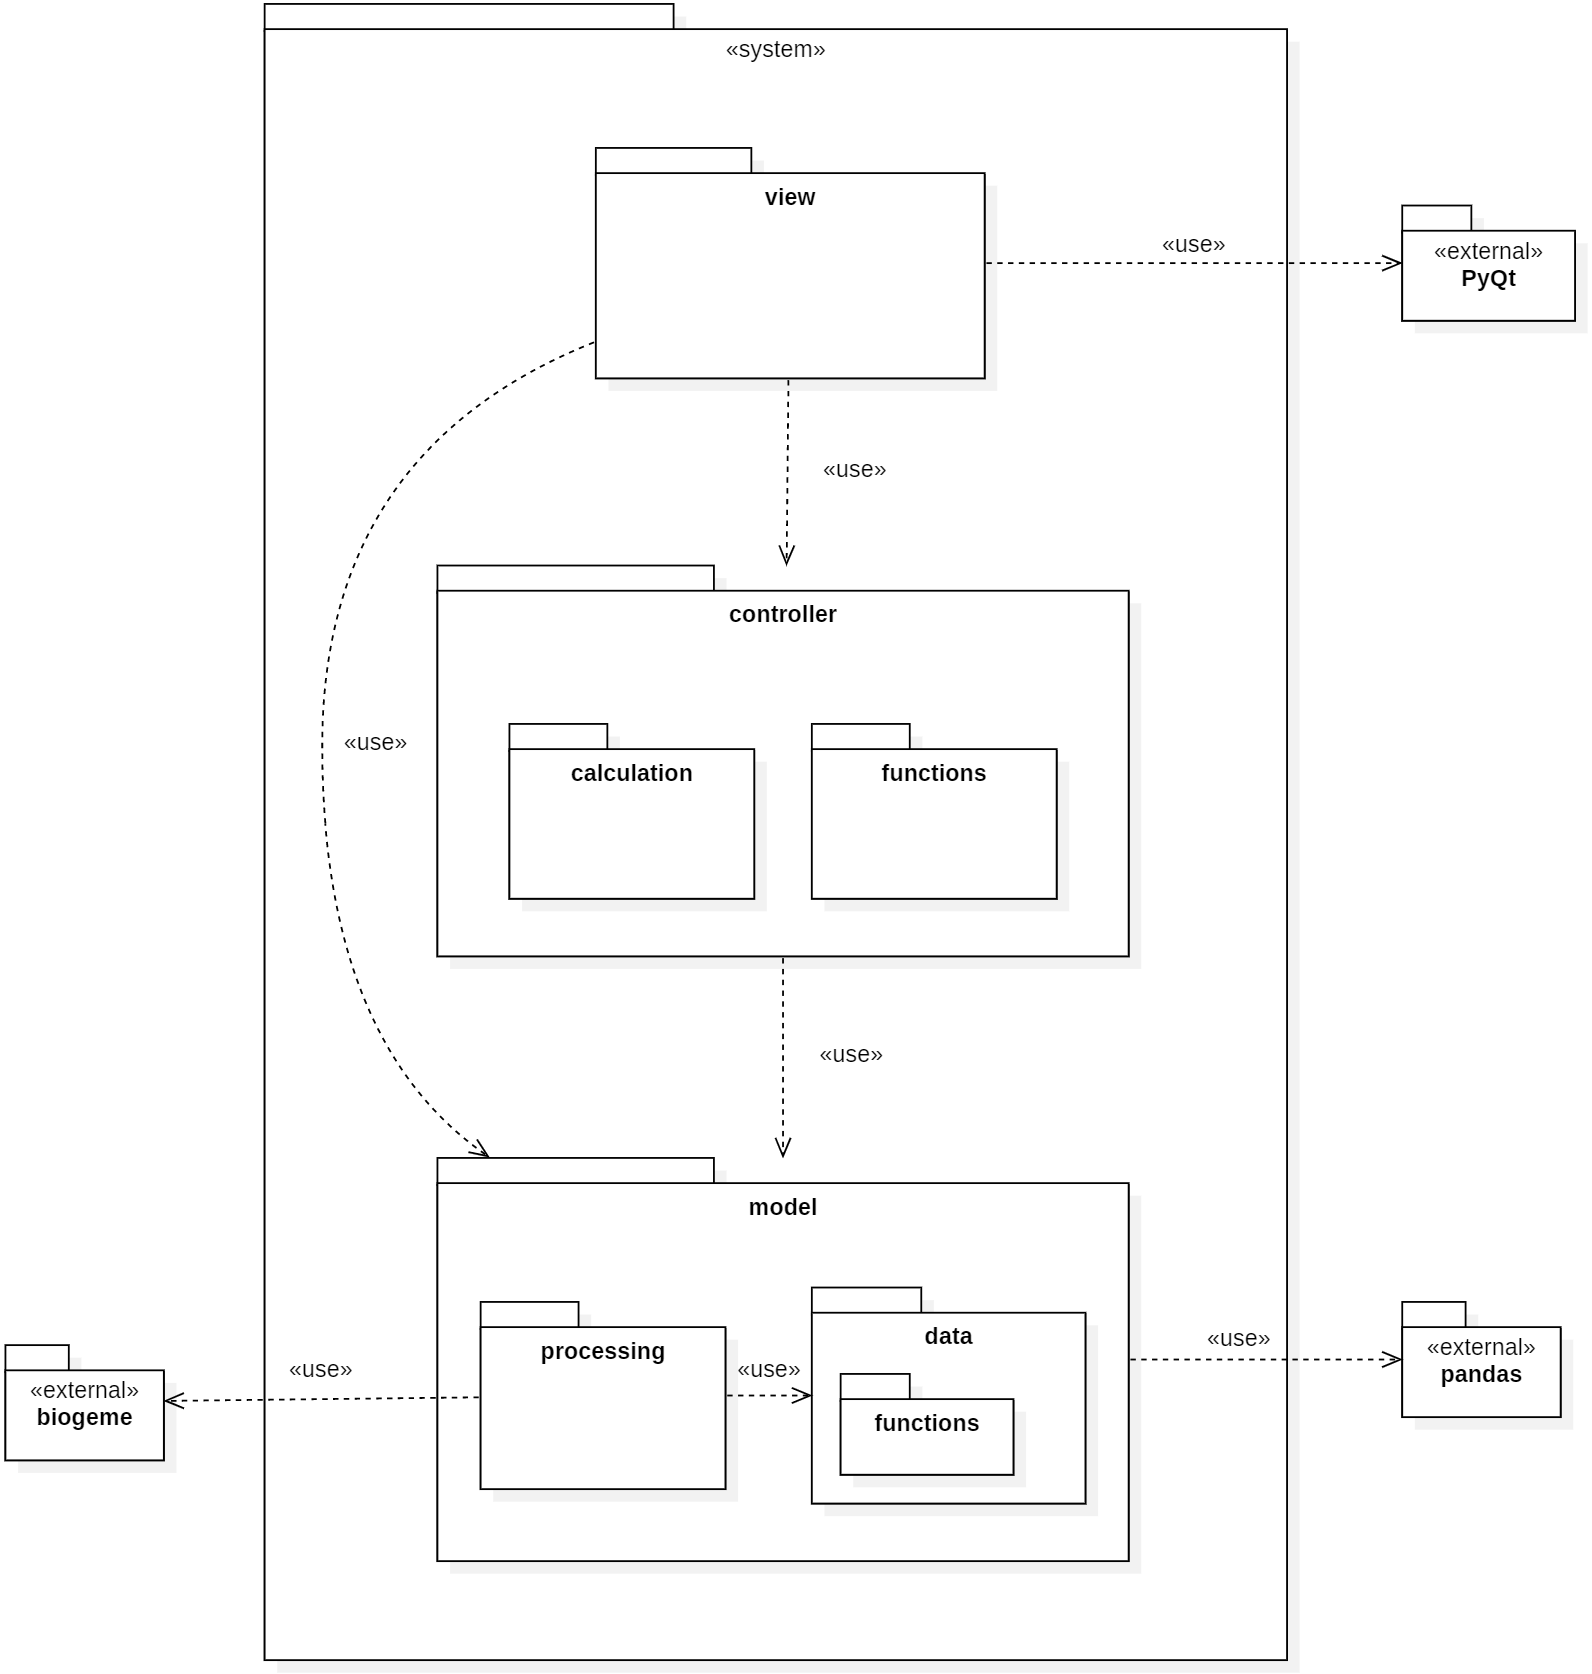
\includegraphics[width=13cm]{img/PackageDiagram.png}
    \caption{Paketdiagramm}
\end{figure}

\begin{itemize}
\item Die Software wird nach dem Prinzip der MVC-Architektur entworfen und setzt sich zusammen aus der View, dem Controller und dem Model.
\end{itemize}

\subsection{View}
\begin{itemize}
\item Die View ist verantwortlich für die visuelle Präsentation der im Model vorhandenen Daten. Dafür greift die View auf das externe Paket \textit{\textbf{PyQt}} zu. Diese wird für die Erstellung der graphischen Benutzeroberfläche verwendet.
\item Nutzereingaben werden immer über \textbf{Controller} weitergeleitet. Somit kann eine schwache Kopplung zum \textbf{Model} beibehalten werden.
\item Da die View auf Erweiterungen des \textbf{Models} reagieren muss, kann eine Abhängigkeit allerdings nicht vermieden werden.
\end{itemize}

\subsection{Controller}
\begin{itemize}
\item Die Controller sind dafür zuständig, die Nutzereingaben aus der View an das Model weiterzuleiten.
\item Finden Änderungen im Model statt, so senden die betroffenen Klassen der View update-Aufrufe über die Controller aus. Dabei werden die betroffenen Daten aus dem Model zurückgegeben.
\item \textbf{Calculation-Paket}: Enthält Controller, die bei der Konfiguration der Berechnung oder beim Umgang mit dem Ergebnis aufgerufen werden.
\item \textbf{Functions-Paket}: Controller, die beim Bearbeiten von Alternativen und
Attributsableitungen aufgerufen werden.
\end{itemize}

\subsection{Model}
\begin{itemize}
\item Das Model umfasst die Datenhaltung und Manipulation dieser Daten bei einem geöffneten Projekt.
\item Bei Änderungen ist das Model zudem verantwortlich vergangene Eingaben zu speichern. Diese sollen anhand einer undo-/redo-Funktion wieder aufrufbar sein.
\item Das externe Python Paket \emph{\textbf{pandas}} wird für die Haltung tabellarischer, vom Nutzer nicht veränderbarer Daten verwendet.
\item \textbf{Processing-Paket}: Umschließt die Funktionalität, welche mit der Konfiguration der Berechnung oder dem Ergebnis zu tun hat. Es existiert eine Schnittstelle, über welche die tatsächliche Berechnung stattfinden kann. Hier wird standardmäßig das externe Python Paket \emph{\textbf{biogeme}} verwendet.
\item \textbf{Data-Paket}: Umfasst jegliche Funktionalität, die für die Datenhaltung und Änderung des Verkehrsmodells zuständig ist.
\item \textbf{Functions-Paket}: Unterpaket von \textbf{Data}. Umfasst spezifisch den Teil des Modells, in welchem die Ausdrücke und Funktionen der Attributsableitungen und Alternativen gehandhabt werden.
\end{itemize}

\newpage
\section{Klassenstruktur}
Im folgenden Abschnitt werden die einzelnen Klassen der Entwurfs dokumentiert, aufgeteilt nach den Paketen. Das gesamte Klassendiagramm, indem alle Klassen aller Pakete abgebildet sind befindet sich im Anhang. In diesem Kapitel sind alle genannten Attribute \emph{private} und alle Methoden \emph{public} soweit nicht explizit anders angegeben. Triviale Funktionen wie einfache \emph{get} und \emph{set} Methoden, sowie triviale Konstruktoren werden nicht genannt.

\subsection{View}
\begin{figure}[H]%
    \centering
    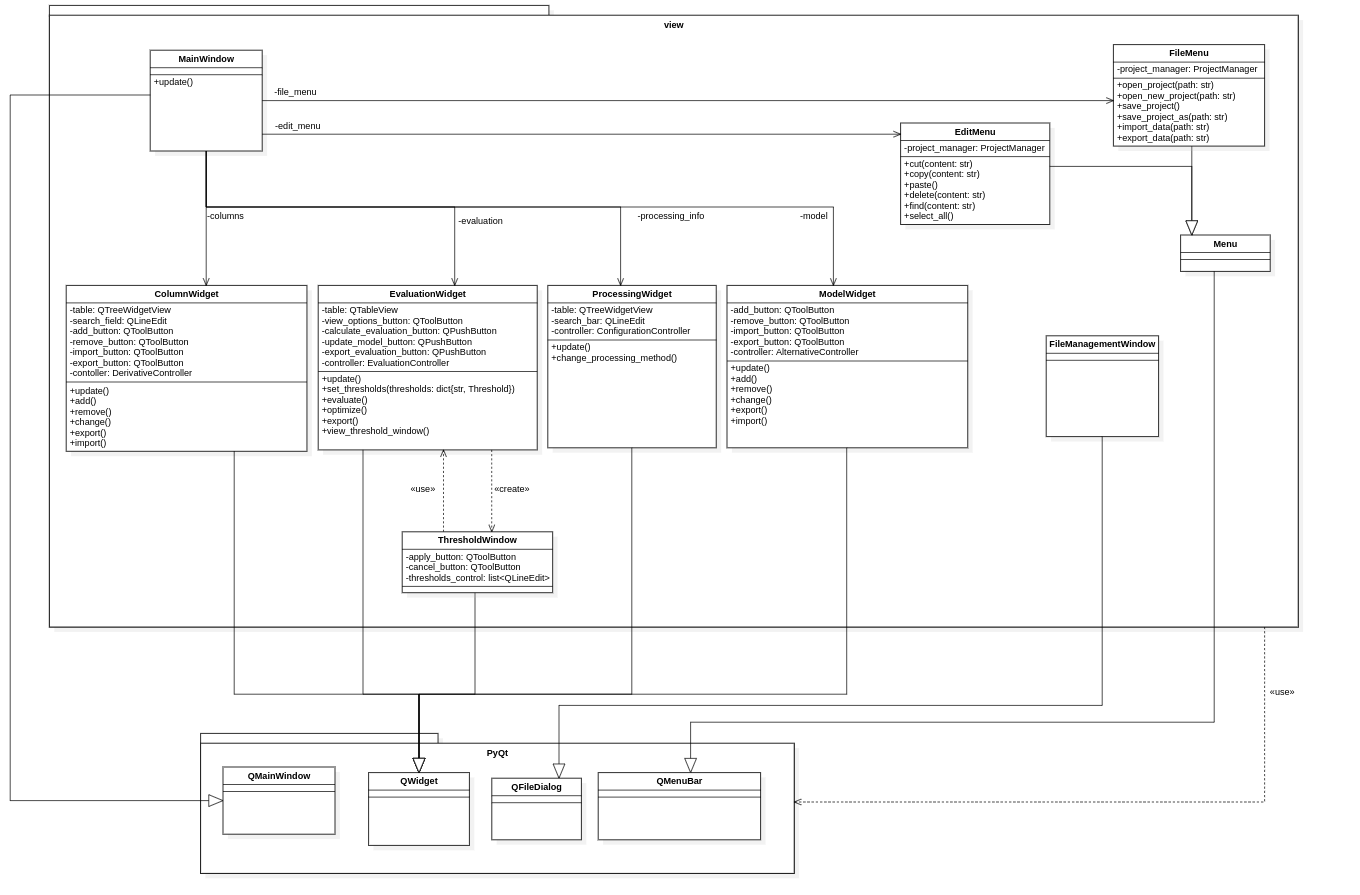
\includegraphics[width=15cm]{entwurf/Entwurf_dokument/img/Alissa/View.png}
    \caption{Das Paket View und seine Klassen mit dem PyQt-Paket}
\end{figure}
Im Paket View sind alle Funktionalitäten enthalten, die zur Realisierung der GUI beitragen. Für die graphische Schnittstelle wird PyQt benutzt. Aus diesem Grund erben die Klassen in dem View ihre Funktionalität und Struktur aus Klassen in PyQt Paket. Im folgenden erfolgt die ausführliche Beschreibung und Erklärung der einzelnen Klassen.

\newpage
\textbf{\large{MainWindow}}\\\\
\begin{figure}[H]%
    \centering
    \begin{minipage}[b]{0.4\textwidth}
        \centering
        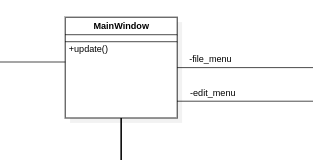
\includegraphics[width=8cm]{entwurf/Entwurf_dokument/img/Alissa/MainWindow.png}
        \caption{Die Klasse MainMenu}
    \end{minipage}
    \hfill
    \begin{minipage}[b]{0.4\textwidth}
        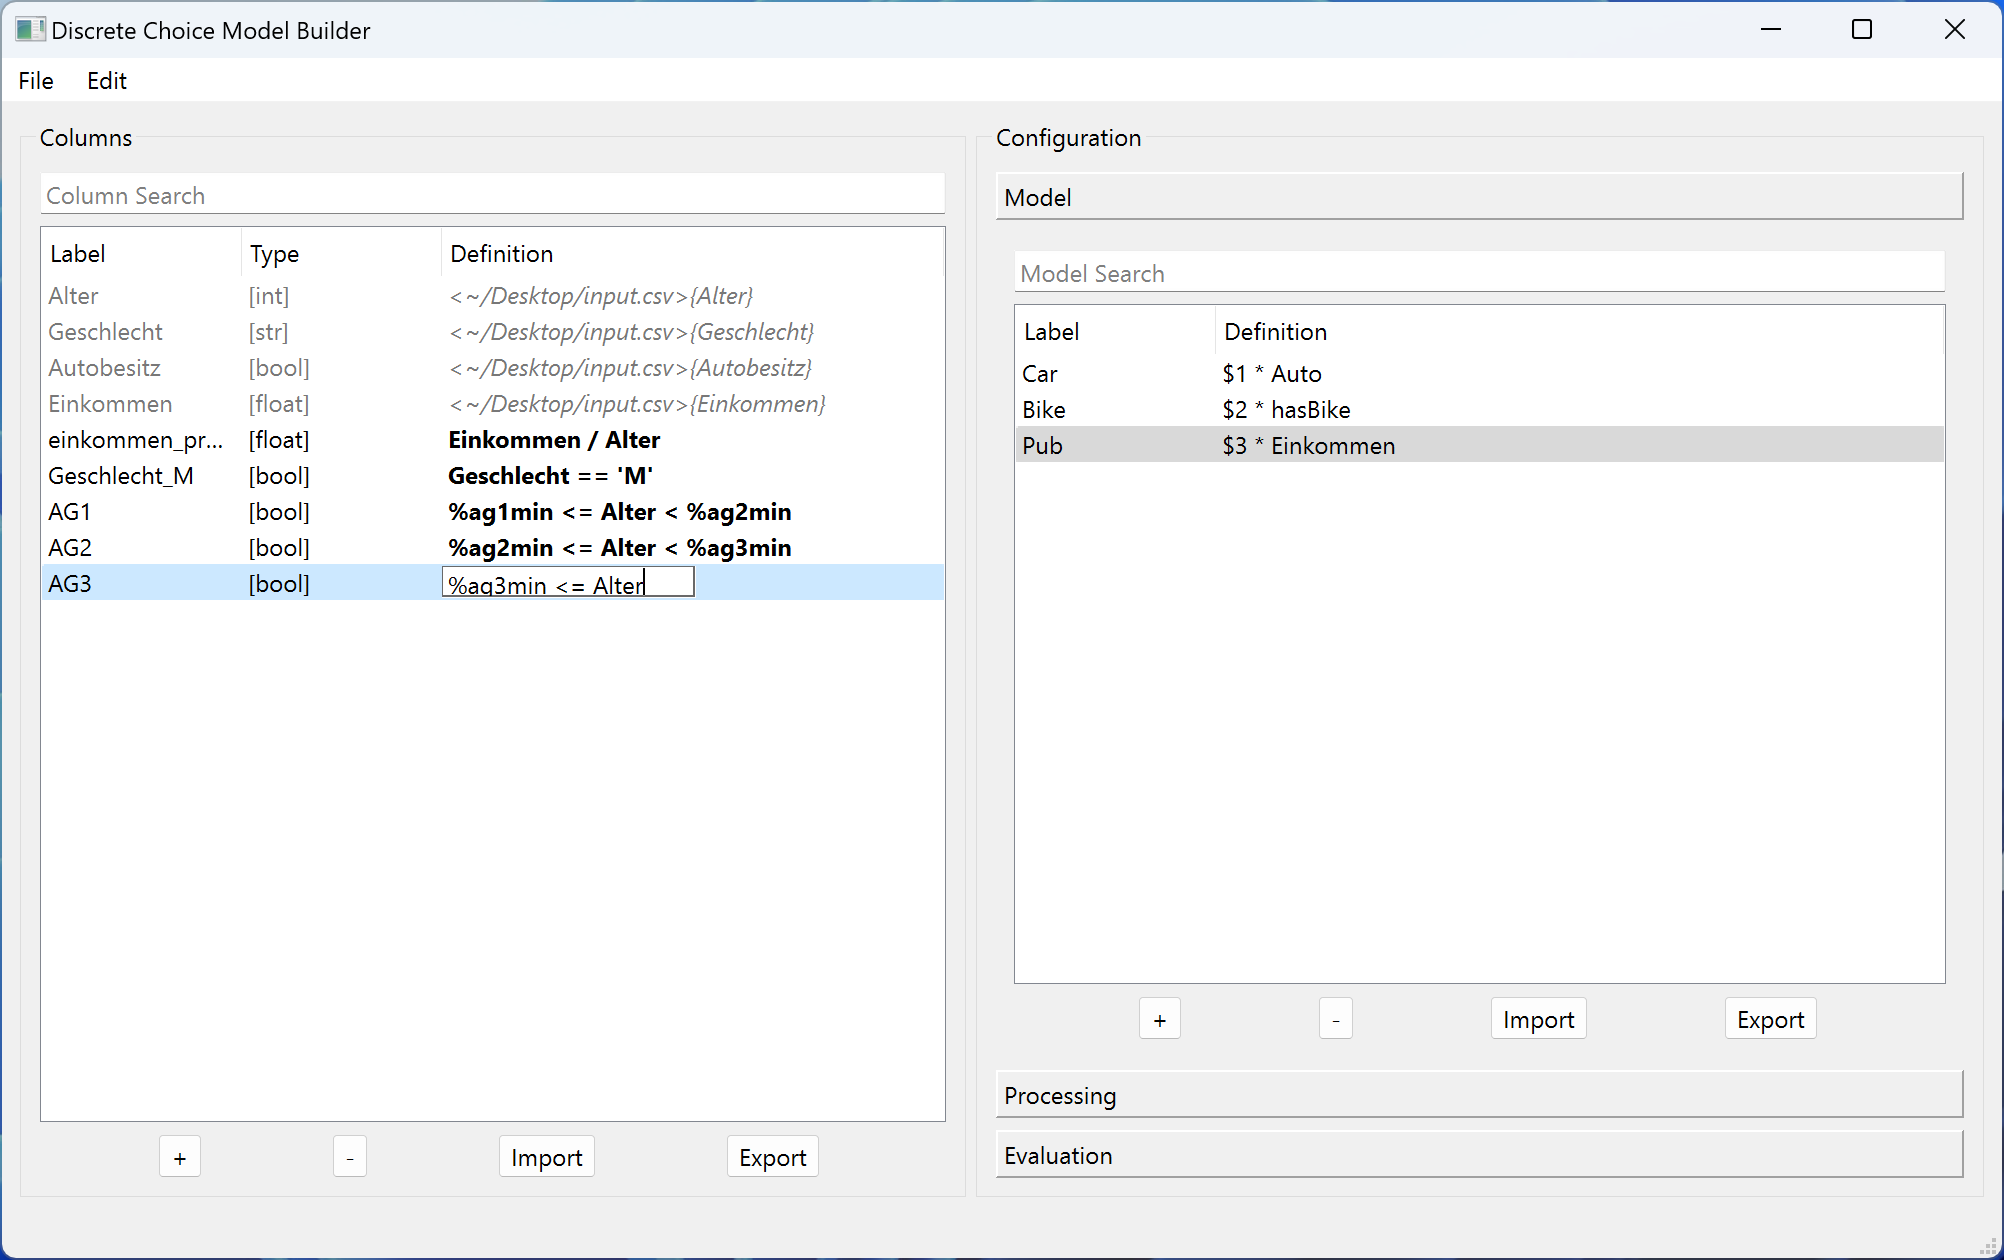
\includegraphics[width=8cm]{specifications/img/gui-screenshots/columns-editing+model.png}
        \caption{Die Klasse MainMenu}
    \end{minipage}
\end{figure}
Dies repräsentiert das Hauptfenster. In dem befinden sich alle graphischen Elemente (Bspw. Tabellen, Menüs, Knöpfe usw.) Die einzelnen Elemente werden je in ihre eigene Klasse spezifiziert, dies erleichtert die Refaktorisierung und das nachträgliche Hinzufügen neuer graphischen Elemente.

Die Klasse erbt von PyQt-QMainWindow. Weitere Informationen finden Sie in den entsprechenden \href{https://doc.qt.io/qt-6/qmainwindow.html}{PyQt-Docs}.
\newline \newline

\textbf{{Attribute}}
NOTIZ: Ich finde die Klassenbezeichnung "PyQt-QMainWindow" etwas unglücklich. "pyqt.QMainWindow" wäre besser.
NOTIZ: Datentypen fehlen!
\begin{itemize}
\item \texttt{file\char`_menu} \newline Repräsentiert das \textit{File Menu} in der GUI
\item \texttt{edit\char`_menu} \newline Repräsentiert das \textit{Edit Menu} in der GUI
\item \texttt{columns} \newline Repräsentiert die Tabelle mit den Erhebungsdaten und Ableitungen. In der GUI befindet sie sich links im Hauptfenster.
\item \texttt{evaluation} \newline Repräsentiert das Teilfenster, wo die Ergebnisse der Berechnungen gezeigt werden.
\item \texttt{processing\char`_info} \newline repräsentiert den Abschnitt aus der GUI, wo die ausgewählte Konfiguration und varablen gesehen werden.
\item \texttt{model} \newline steht für den Abschnitt \textit{Model}, wo die Alternativen zu sehen sind.
\end{itemize}

\textbf{{Methoden}}
\begin{itemize}
\item \texttt{update()} \newline Dient zur Aktualisierung der GUI, wenn ein Befehl aus dem \textit{File Menu} oder \textit{Edit Menu} ausgefüht wird und dies die angezeigten Daten ändert.
\\\\
\underline{{Parameter}}
\begin{tabular}{lll}
 keine \\
\end{tabular}

\underline{{Rückgabewert}}
\begin{tabular}{lll}
 keine \\
\end{tabular}
\end{itemize}

\newpage
\textbf{\large{Menu}}\\\\
\begin{figure}[H]%
    \centering
    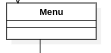
\includegraphics[width=4cm]{entwurf/Entwurf_dokument/img/Alissa/Menu.png}
    \caption{Die Klasse Menu}
\end{figure}
Dies steht für eine Menü in der Menüleiste. Die einzelnen Menüs haben gemeinsame Eigenschaften (gleiche grobe Strucktur), aber jede Menü bietet dem Nutzer unterschiedliche Operationen. Aus diesem Grund wird für jede spezielle Menü eine eigene Klasse erstellt.
Die Klasse \textit{Menu} erbt von PyQt-QMenuBar. Für weitere Informationen sehen Sie \href{https://doc.qt.io/qtforpython-5/PySide2/QtWidgets/QMenuBar.html}{PyQt-Docs}
\newline \newline

\textbf{{Attribute}}
\begin{itemize}
\item[] keine eigene Attribute \newline
\end{itemize}
    
\textbf{{Methoden}}
\begin{itemize}
\item[] keine eigene Methoden
\end{itemize}

\newpage
\textbf{\large{FileMenu}}\\\\
\begin{figure}[H]%
    \centering
    \begin{minipage}[b]{0.4\textwidth}
        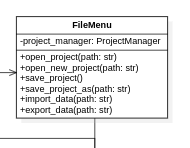
\includegraphics[width=5cm]{entwurf/Entwurf_dokument/img/Alissa/FileMenu.png}
        \caption{Die Klasse FileMenu}
    \end{minipage}
    \hfill
    \begin{minipage}[b]{0.4\textwidth}
        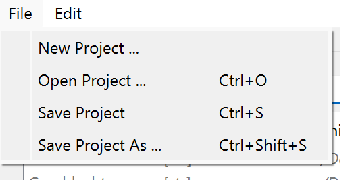
\includegraphics[width=6cm]{entwurf/Entwurf_dokument/img/Alissa/EditMenuGUI.png} %Aus versehen anders benannt. Sollte eig. FileMenuGUI heißen
    \caption{Die \textit{File Menu} im GUI. NICHT 1 ZU 1 IST DAS OK?}
    \end{minipage}
\end{figure}
Die Klasse FileMenu ist die realisierung der \textit{File Menu} aus der graphischen Schnittstelle. Sie erbt ihre grobe Strucktur aus der Klasse \textit{Menu}. Die \textit{File Menu} bietet dem Nutzer die Möglichkeit, das Projekt zu verwalten (importieren, speichern usw.)
\newline \newline

NOTIZ: Datentypen fehlen! Funktionen mit () versehen!
\textbf{{Attribute}}
\begin{itemize}
\item \texttt{project\char`_manager} \newline Das ist der Controller. Mit dem kann die Projekt Verwaltung umgestzt werden.
\end{itemize}

\textbf{{Methoden}}
\begin{itemize}
\item \texttt{open\char`_project} \newline Diese Option ermöglicht dem Nutzer, einen bereitsexistierenden Projekt zu öffnen.
\\\\
\underline{{Parameter}}
\begin{tabular}{lll}
 & \texttt{path} & Der Dateipfad(String), wo das Projekt gespeichert ist. \\
\end{tabular}

\underline{{Rückgabewert}}
\begin{tabular}{lll}
 keine \\
\end{tabular}

\item \texttt{open\char`_new\char`_project} \newline ermöglicht dem Nutzer, eine neues Projekt zu öffnen
\\\\
\underline{{Parameter}}
\begin{tabular}{lll}
 & \texttt{path} & Der Dateipfad(String), wo das Projekt geöffnet und gespeichert werden soll. \\
\end{tabular}

\underline{{Rückgabewert}}
\begin{tabular}{lll}
 keine \\
\end{tabular}

\item \texttt{save\char`_project} \newline ermöglicht dem Nutzer, das geöffnete Projekt zu speichern.
\\\\
\underline{{Parameter}}
\begin{tabular}{lll}
 keine \\
\end{tabular}

\underline{{Rückgabewert}}
\begin{tabular}{lll}
 keine \\
\end{tabular}

\item \texttt{save\char`_project\char`_as} \newline damit kann der Nutzer das geöffnete Projekt, in einem  anderen Dateipfad zu speichern.
\\\\
\underline{{Parameter}}
\begin{tabular}{lll}
 & \texttt{path} & Der Dateipfad(String), wo das Projekt gespeichert werden soll. \\
\end{tabular}

\underline{{Rückgabewert}}
\begin{tabular}{lll}
 keine \\
\end{tabular}

\item \texttt{import\char`_data} \newline Mit dem wird das Laden einer CSV Datei mit den Erhebungsdaten ermöglicht.
\\\\
\underline{{Parameter}}
\begin{tabular}{lll}
 & \texttt{path} & Der Dateipfad, wo der CSV Datei sich befindet. AUch vom Typ String \\
\end{tabular}

\underline{{Rückgabewert}}
\begin{tabular}{lll}
 keine \\
\end{tabular}

\item \texttt{export\char`_data} \newline Mit dieser Option, kann die Tabelle mit den Erhebungsdaten und Ableitungen als eine  Tabelle exportiert werden (TYP)?
\\\\
\underline{{Parameter}}
\begin{tabular}{lll}
 & \texttt{path} & Der Dateipfad(String), wo die CSV Datei exportiert wird. \\
\end{tabular}

\underline{{Rückgabewert}}
\begin{tabular}{lll}
 keine \\
\end{tabular}
\end{itemize}

\newpage
\textbf{\large{EditMenu}}\\\\
\begin{figure}[H]%
    \centering
    \begin{minipage}[b]{0.4\textwidth}
        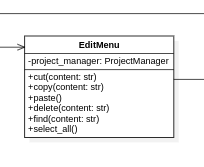
\includegraphics[width=5cm]{entwurf/Entwurf_dokument/img/Alissa/EditMenu.png}
        \caption{Die Klasse EditMenu}
    \end{minipage}
    \hfill
    \begin{minipage}[b]{0.4\textwidth}
        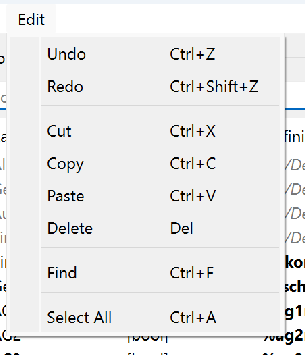
\includegraphics[width=6cm]{entwurf/Entwurf_dokument/img/Alissa/FileMenuGUI.png} %Aus versehen anders benannt. Sollte eig. EditMenuGUI heißen
        \caption{Die \textit{Edit Menu} im GUI. NICHT 1 ZU 1 IST DAS OK?}
    \end{minipage}
\end{figure}
Di Klasse \textit{EditMenu} repräsentiert das \textit{Edit Menu} in der GUI. Sie erbt von der Klasse \textit{Menu} und bietet dem Nutzer Operationen, womit er das Arbeit mit dem Projekt effezient wird. Zum Beispiel \textit{undo} und \textit{redo}
\newline \newline

NOTIZ: Datentypen fehlen! Funktionen mit () versehen!
\textbf{{Attribute}}
\begin{itemize}
\item \texttt{project\char`_manager} \newline Der Controller, der für Projekt Managment verantwörtlich ist.
\end{itemize}

\textbf{{Methoden}}
\begin{itemize}
\item \texttt{undo} \newline Das zueltzt ausgeführte Aktion wird rückgängig gemacht.
\\\\
\underline{{Parameter}} 
\begin{tabular}{lll}
 keine
\end{tabular}

\underline{{Rückgabewert}}
\begin{tabular}{lll}
 keine
\end{tabular}

\item \texttt{redo} \newline Das \texttt{undo} rückgängig machen. (BESSER BESCHREIBUNG?)
\\\\
\underline{{Parameter}} 
\begin{tabular}{lll}
 keine
\end{tabular}

\underline{{Rückgabewert}}
\begin{tabular}{lll}
keine
\end{tabular}

\item \texttt{cut} \newline Einen ausgewählten Inhalt(Text) ausschneiden.
\\\\
\underline{{Parameter}} 
\begin{tabular}{lll}
 & \texttt{content} & Ist vom Typ String und bezeichnet den Inhalt zum Ausschneiden\\
\end{tabular}

\underline{{Rückgabewert}}
\begin{tabular}{lll}
keine
\end{tabular}

\item \texttt{copy} \newline Ausgewählte bzw. makierte Inhalt(Text) kopieren.
\\\\
\underline{{Parameter}} 
\begin{tabular}{lll}
& \texttt{content} & Ist vom Typ String und bezeichnet den zu kopierenden Inhalt \\
\end{tabular}

\underline{{Rückgabewert}}
\begin{tabular}{lll}
keine
\end{tabular}

\item \texttt{paste} \newline Einen zuvor kopierten oder ausgeschnittenen Inhalt(Text) einfügen.
\\\\

\underline{{Parameter}} 
\begin{tabular}{lll}
keine
\end{tabular}

\underline{{Rückgabewert}}
\begin{tabular}{lll}
keine
\end{tabular}

\item \texttt{delete} \newline Einen vom Nutzer ausgewählten Inhalt(Text) löschen.
\\\\
\underline{{Parameter}} 
\begin{tabular}{lll}
& \texttt{content} & Der Inhalt(String), was gelöscht werden soll. \\
\end{tabular}

\underline{{Rückgabewert}}
\begin{tabular}{lll}
keine
\end{tabular}

\item \texttt{find} \newline Einen bestimmten Inhalt(Text) in den Tabellen (Attributsableitungen, Alternativen oder Ergebnisse der Berechnungen) suchen.
\\\\
\underline{{Parameter}} 
\begin{tabular}{lll}
 & \texttt{content} & Der Inhalt(String), wonach gesucht werden soll. \\
\end{tabular}

\underline{{Rückgabewert}}
\begin{tabular}{lll}
 keine
\end{tabular}

\item \texttt{select\char`_all} \newline WAS WIRD AUSGEWÄHLT?
\\\\
\underline{{Parameter}} 
\begin{tabular}{lll}
keine
\end{tabular}

\underline{{Rückgabewert}}
\begin{tabular}{lll}
 keine
\end{tabular}
\end{itemize}

\newpage
\textbf{\large{FileMangamentWindow}}\\\\
\begin{figure}[H]%
    \centering
    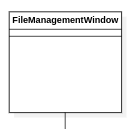
\includegraphics[width=5cm]{entwurf/Entwurf_dokument/img/Alissa/FileManagmentWindow.png}
    \caption{Die Klasse FileManagmentWindow}
\end{figure}
Die Klasse \textit{FileManagmentWindow} repräsentiert das Datei-Dialog. Das Fenster, womit der Nutzer die Dateien (CSV oder JSON) aussuchen und wählen kann. Diese Klasse erbt von \textit{QFileDialog}, dessen Informationen auf \href{https://doc.qt.io/qtforpython-5/PySide2/QtWidgets/QFileDialog.html}{PyQt Docs}. Die \textit{QFileDialog} implementiert das Datei-Dialog. Die Kindesklasse \textit{FileManagmentWindow} benötigt keine spezielle Eigenschaften, weswegen keine neue Methoden oder Attribute hinzukommen.
\newline \newline

\textbf{{Attribute}}
\begin{itemize}
\item[] keine eigene Attribute
\end{itemize}

\textbf{{Methoden}}
\begin{itemize}
\item[] keine eigene Methoden
\end{itemize}

\newpage
\textbf{\large{ColumnWidget}}\\\\
\begin{figure}[H]%
    \centering
    \begin{minipage}[b]{0.4\textwidth}
        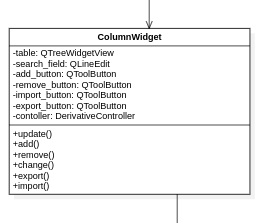
\includegraphics[width=5cm]{entwurf/Entwurf_dokument/img/Alissa/ColumnWidget.png}
        \caption{Die Klasse ColumnWidget}
    \end{minipage}
    \hfill
    \begin{minipage}[b]{0.4\textwidth}
        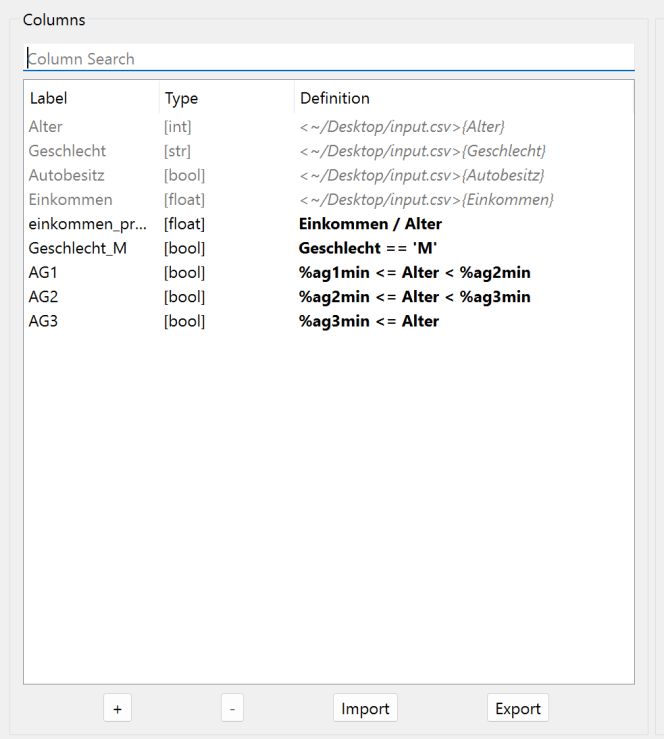
\includegraphics[width=5cm]{entwurf/Entwurf_dokument/img/Alissa/Columns.png} 
    \caption{Die \textit{Columns} im GUI.}
    \end{minipage}
\end{figure}
\textit{ColumnWidget} Repräsentiert die Tabelle in der GUI, wo die Spalten aus dem Erhebubgsdaten und die Ableitungen gezeigt werden. Außerdem erbt diese Klasse von QWidget aus der PyQt Biblothek.  Das ist die Basis Klasse für alle Objekte, die Nutzerinterktion ermöglichen. Weiter Informationen sind auf \href{https://doc.qt.io/qt-6/qwidget.html}{PyQt Docs} zu finden.
\newline \newline

NOTIZ: Datentypen fehlen! Funktionen mit () versehen!
\textbf{{Attribute}}
\begin{itemize}
\item \texttt{table} \newline steht für die Tabelle mit den Attributen
\item \texttt{search\char`_field} \newline steht für den Suchfeld. in der GUI ist dies oberhalb der Tabelle \textit{table}
\item \texttt{add\char`_button} \newline damit wird die \textit{add "+"} Schaltfläche relisiert, womit der Nutzer einen Attribute hinzufügen kann.
\item \texttt{remove\char`_button} \newline steht für den \textit{remove "\textendash"} Schaltfläche. Mit dem kann der Nutzer eine Attributsableitung hinzufügen. 
\item \texttt{import\char`_button} \newline Diese Schaltfläche emöglicht dem Nutzer, Attributsableitungen zu importieren.
\item \texttt{export\char`_button} \newline Mit dierser Schlatfläche kann der Nutzer ausgewählte Attributsableitungen exportieren (Als CSv oder JSON)
\item \texttt{controller} \newline Das ist der Controller (Typ \textit{DerivativeController}), mit dem die Nutzeranfragen bzgl. der Verwaltung von Attributsableitungen umgesetzt werden können.
\end{itemize}

\textbf{{Methoden}}
\begin{itemize}
\item \texttt{update} \newline aktualisiert die Anzeige sobald Änderungen am Model vorgenommen wurden bspw. Fehler wurde bei der Eingabe erkannt und muss hervorgehoben werden.
\\\\
\underline{{Parameter}} 
\begin{tabular}{lll}
 keine
\end{tabular}

\underline{{Rückgabewert}}
\begin{tabular}{lll}
keine
\end{tabular}
\item \texttt{add} \newline Gibt dem Nutzer die Möglichkeit, in der Tabelle eine Attributsableitung hinzuzufügen.
\\\\
\underline{{Parameter}} 
\begin{tabular}{lll}
keine
\end{tabular}

\underline{{Rückgabewert}}
\begin{tabular}{lll}
keine
\end{tabular}
\item \texttt{remove} \newline Gibt dem Nutzer die Möglichkeit, in der Tabelle eine Ableitung zu löschen
\\\\
\underline{{Parameter}} 
\begin{tabular}{lll}
keine (WARUM KEINE?)
\end{tabular}

\underline{{Rückgabewert}}
\begin{tabular}{lll}
 keine
\end{tabular}
\item \texttt{change} \newline Mit dieser Funktion kann das Ändern einer Attributsableitung dem Nutzer ermöglicht werden.
(FRAGE: BRAUCHEN CHANGE UND REMOVE KEINE PARAMETER?)
\\\\
\underline{{Parameter}} 
\begin{tabular}{lll}
keine (WARUM KEINE?)
\end{tabular}

\underline{{Rückgabewert}}
\begin{tabular}{lll}
keine
\end{tabular}
\item \texttt{export} \newline steht für das exportieren von Attributsableitungen
\\\\
\underline{{Parameter}} 
\begin{tabular}{lll}
keine (WARUM KEINE?)
\end{tabular}

\underline{{Rückgabewert}}
\begin{tabular}{lll}
 & \texttt{type} & Description\\
\end{tabular}
\item \texttt{import} \newline steht für das importieren von Attributsableitungen
\\\\
\underline{{Parameter}} 
\begin{tabular}{lll}
keine (WARUM KEINE?)
\end{tabular}

\underline{{Rückgabewert}}
\begin{tabular}{lll}
keine
\end{tabular}
\end{itemize}

\newpage
\textbf{\large{EvaluationWidget}}\\\\
\begin{figure}[H]%
    \centering
    \begin{minipage}[b]{0.4\textwidth}
        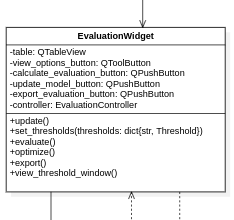
\includegraphics[width=5cm]{entwurf/Entwurf_dokument/img/Alissa/EvaluationWidget.png}
        \caption{Die Klasse EvaluationWidget}
    \end{minipage}
    \hfill
    \begin{minipage}[b]{0.4\textwidth}
        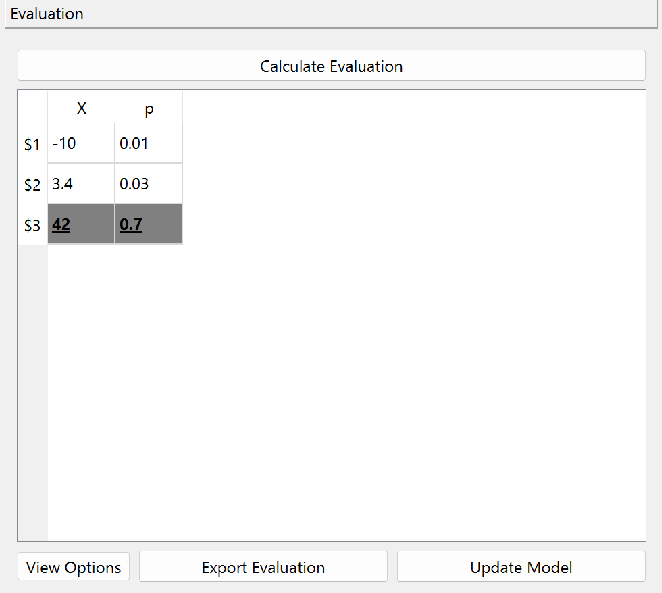
\includegraphics[width=5cm]{entwurf/Entwurf_dokument/img/Alissa/evaluationGUI.png} 
    \caption{Die \textit{Evaluation} Fenster im GUI.}
    \end{minipage}
\end{figure}
Die Klasse \textit{EvaluationWidget} enthält die Eigenschaften und Funktionen/Operationen, damit die Tabelle der Auswertung relisiert wird. Außerdem erbt die Klasse von der \textit{PyQT} Klasse \textit{QWidget}. In der \href{https://doc.qt.io/qt-6/qwidget.html}{QWidget\textendash Docs} sind ausführliche Informationen über diese PyQT\textendash Klasse.
\newline \newline

NOTIZ: Datentypen fehlen! Funktionen mit () versehen!
\textbf{{Attribute}}
\begin{itemize}
\item \texttt{table} \newline Tabelle, welche die Ergebnisse der Auswertung enthält
\item \texttt{view\char`_options\char`_button} \newline zeigt das Fenster, wo der Nutzer den Schwellwert ändern kann.
\item \texttt{calculate\char`_evaluation\char`_button} \newline Das ist die Schaltfläche, mit dem das Auswerten betätigt wird.
\item \texttt{update\char`_model\char`_button} \newline Es aktualisiert das Model (ERKLÄRUNG IST NICHT TOLL)
\item \texttt{export\char`_evaluation\char`_button} \newline Ermöglicht dem Nutzer, die Ergebnisse der Auswertung zu exportieren.
\item \texttt{controller} \newline Der Controller, worüber mit dem Model kommuniziert wird, um die Nutzeranfragen bzgl. der Auswertung umzusetzen.
\end{itemize}

\textbf{{Methoden}}
\begin{itemize}
\item \texttt{update} \newline aktualisiert die Nutzeranzeige, wenn was am Model geändert wird (Bsp. Nach dem der Schwellwertänderung erfolgreich umgesetzt wurde)
\\\\
\underline{{Parameter}} 
\begin{tabular}{lll}
keine
\end{tabular}

\underline{{Rückgabewert}}
\begin{tabular}{lll}
keine
\end{tabular}

\item \texttt{set\char`_thresholds} Dadurch kann der Schwellwert geändert werden. (ERKLÄRUNG MUSS VERBESSERT WERDEN) \newline 
\\\\
\underline{{Parameter}} 
\begin{tabular}{lll}
 & \texttt{thresholds} & NOCH UNKLAR \\
\end{tabular}

\underline{{Rückgabewert}}
\begin{tabular}{lll}
keine
\end{tabular}

\item \texttt{evaluate} \newline die Methode führt die Auswertung aus.
\\\\
\underline{{Parameter}} 
\begin{tabular}{lll}
keine
\end{tabular}

\underline{{Rückgabewert}}
\begin{tabular}{lll}
keine
\end{tabular}

\item \texttt{optimize} \newline führt Optimierugn des Models aus
\\\\
\underline{{Parameter}} 
\begin{tabular}{lll}
keine
\end{tabular}

\underline{{Rückgabewert}}
\begin{tabular}{lll}
keine
\end{tabular}

\item \texttt{export} \newline exportiert die Ergebnisse der Auswertung 
\\\\
\underline{{Parameter}} 
\begin{tabular}{lll}
 keine (HIER MUSS EIN SPEICHERORT ANGEGEBEN WERDEN)
\end{tabular}

\underline{{Rückgabewert}}
\begin{tabular}{lll}
keine
\end{tabular}

\item \texttt{view\char`_threshold\char`_window} \newline zeigt dem Nutzer das Fenster, wo er den Schwellwert eingeben und anwenden kann. Hierfür wird ein Objekt der Klasse \textit{ThresholdWindow} erstellt.
\\\\
\underline{{Parameter}} 
\begin{tabular}{lll}
keine
\end{tabular}

\underline{{Rückgabewert}}
\begin{tabular}{lll}
keine
\end{tabular}
\end{itemize}

\newpage
\textbf{\large{ThresholdWindow}}\\\\
\begin{figure}[H]%
    \centering
    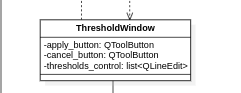
\includegraphics[width=5cm]{entwurf/Entwurf_dokument/img/Alissa/ThresholdWindow.png}
    \caption{Die Klasse ThresholdWidget}
\end{figure}
Diese Klasse repräsentiert das Fenster, wo der Nutzer den Schwellwert eingeben und anwenden kann. \textit{ThresholdWindow} erbt von PyQt\textendash QWidget. In der \href{https://doc.qt.io/qt-6/qwidget.html}{Dokumentation} von \textit{QWidget} sind weitere Informationen über diese Klasse zu finden. Die ThresholdWindow benutzt die Funktion \texttt{set\char`_threshold(thresholds)} aus der Klasse \textit{EvaluationWidget}, um den Schwellwert anzuwenden.
\newline \newline

NOTIZ: Datentypen fehlen! Funktionen mit () versehen!
\textbf{{Attribute}}
\begin{itemize}
\item \texttt{apply\char`_button} \newline Die Schaltfläche, womit der Nutzer das Anwenden des Schwellwertes betätigen kann.
\item \texttt{cancle\char`_button} \newline Die Schaltfläche, womit der Nutzer den Vorgang abbricht (Das heißt kein Schwellwert wird angewendet) und zurück zum Hauptfenster geleitet wird.
    \item \texttt{thresholds\char`_control} \newline UNKLAR
\end{itemize}

\textbf{{Methoden}}
\\keine eigene Methoden

\newpage
\textbf{\large{ProcessingWidget}}\\\\
\begin{figure}[H]%
    \centering
    \begin{minipage}[b]{0.4\textwidth}
        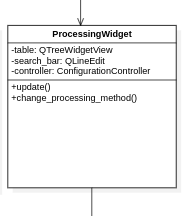
\includegraphics[width=5cm]{entwurf/Entwurf_dokument/img/Alissa/ProcessingWidget.png}
        \caption{Die Klasse ProcessingWidget}
    \end{minipage}
    \hfill
    \begin{minipage}[b]{0.4\textwidth}
        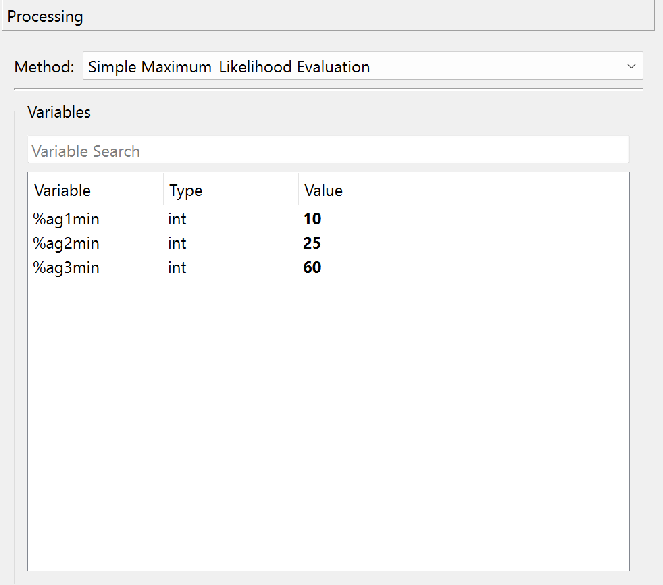
\includegraphics[width=5cm]{entwurf/Entwurf_dokument/img/Alissa/Processing.png} 
    \caption{Die \textit{Processing} Fenster in der GUI.}
    \end{minipage}
\end{figure}
Die Klasse \textit{ProcessingWidget} repräsentiert das Processing Fenster in der GUI, in dem der Nutzer die Methode für die Auswertung wählen kann. Diese Klasse erbt von der Klasse \textit{QWidget} aus dem Paket PyQT. Witere Informationen bezüglich der Klasse QWidget sind in der \href{https://doc.qt.io/qt-6/qwidget.html}{Dokementation} zu finden.
\newline \newline

NOTIZ: Datentypen fehlen! Funktionen mit () versehen!
\textbf{{Attribute}}
\begin{itemize}
\item \texttt{table} \newline steht für die Tabelle in der GUI, wo der Nutzer die Variablen sehen kann.
\item \texttt{search\char`_bar} \newline steht für den Suchfeld. Dadurch kann der Nutzer nach Variablen suchen.
\item \texttt{controller} \newline Das ist der Controller (Typ \textit{ConfiguartionController}), der Nutzeranfragen in der Processing Fenster verarbeitet.
\end{itemize}

\textbf{{Methoden}}
\begin{itemize}
\item \texttt{update} \newline Operation aktualisiert die Anzeige für en Nutzer, falls was am Model geändert wurde (bspw. Der Nutzer hat eine  Ableitung mit neuen Variablen hinzugefügt)
\\\\
\underline{{Parameter}} 
\begin{tabular}{lll}
keine
\end{tabular}

\underline{{Rückgabewert}}
\begin{tabular}{lll}
keine
\end{tabular}
\item \texttt{change\char`_processing\char`_configuration} \newline ändert die Konfiguration für die Berechnungen.
\\\\
\underline{{Parameter}} 
\begin{tabular}{lll}
keine (HIER KANN AUCH EIN PARAMTER KOMMEN)
\end{tabular}

\underline{{Rückgabewert}}
\begin{tabular}{lll}
keine
\end{tabular}
\end{itemize}

\newpage
\textbf{\large{ModelWidget}}\\\\
\begin{figure}[H]%
    \centering
    \begin{minipage}[b]{0.4\textwidth}
        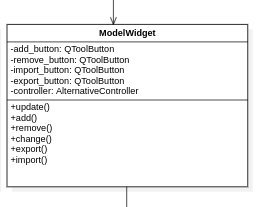
\includegraphics[width=5cm]{entwurf/Entwurf_dokument/img/Alissa/ModelWidget.png}
        \caption{Die Klasse ModelWidget}
    \end{minipage}
    \hfill
    \begin{minipage}[b]{0.4\textwidth}
        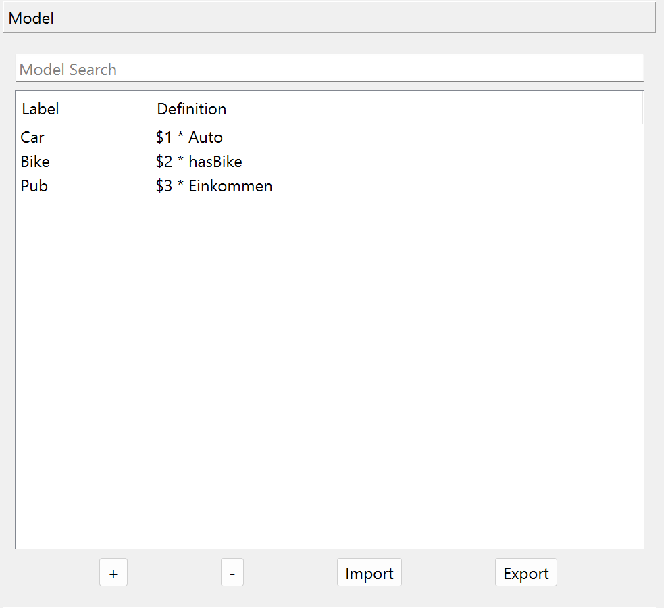
\includegraphics[width=5cm]{entwurf/Entwurf_dokument/img/Alissa/ModelGUI.png} 
    \caption{Die \textit{Model} Fenster in der GUI.}
    \end{minipage}
\end{figure}
Die Klasse \textit{ModelWidget} repräsentiert die Tabelle (im Hauptfenster) mit den Alternativen. Sie erbt von QWidget, dessen Dokumentation \href{https://doc.qt.io/qt-6/qwidget.html}{hier} zu finden ist. 
\newline \newline

\textbf{{Attribute}}
\begin{itemize}
\item \texttt{add\char`_button} \newline Diese Schaltfläche erlaubt dem Nutzer, eine Alternative zu definieren.
\item \texttt{remove\char`_button} \newline Mit dieser Schaltfläche kann der Nutzer eine Alternative löschen
\item \texttt{import\char`_char} \newline ermöglicht dem Nutzer, die Alternativen zu exportieren.
\item \texttt{export\char`_button} \newline ermöglicht dem Nutzer, Alternativen zu importieren.
\item \texttt{controller} \newline Der Controller, der die Nutzeranfragen (Alternativen hinzufügen, löschen usw.) im Model verarbeitet.
\end{itemize}

\textbf{{Methoden}}
\begin{itemize}
\item \texttt{update} \newline aktualisiert dem Nutzer angezeigten Informationen. Bspw. einer der angegebene Alternativen enthält eine unbekannte variable und muss daher akiert werden.
\\\\
\underline{{Parameter}} 
\begin{tabular}{lll}
keine
\end{tabular}

\underline{{Rückgabewert}}
\begin{tabular}{lll}
keine
\end{tabular}

\item \texttt{add} \newline fügt eine neue Alternative hinzu
\\\\
\underline{{Parameter}} 
\begin{tabular}{lll}
keine
\end{tabular}

\underline{{Rückgabewert}}
\begin{tabular}{lll}
keine
\end{tabular}

\item \texttt{remove} \newline löscht eine Alternative aus dem Model
\\\\
\underline{{Parameter}} 
\begin{tabular}{lll}
keine (PARAMETER NÖTIG) \\
\end{tabular}

\underline{{Rückgabewert}}
\begin{tabular}{lll}
keine\\
\end{tabular}

\item \texttt{change} \newline ändert eine schin eingegeben Alternative.
\\\\
\underline{{Parameter}} 
\begin{tabular}{lll}
keine (PARAMETER NÖTIG)\\
\end{tabular}

\underline{{Rückgabewert}}
\begin{tabular}{lll}
keine \\
\end{tabular}

\item \texttt{export} \newline exportiert die Alternativen zu einem Speicherort. 
\\\\
\underline{{Parameter}} 
\begin{tabular}{lll}
keine (PARAMETR NÖTIG)\\
\end{tabular}

\underline{{Rückgabewert}}
\begin{tabular}{lll}
keine\\
\end{tabular}

\item \texttt{import} \newline importiert ALternativen aus einer CSV oder JSON Datei.
\\\\
\underline{{Parameter}} 
\begin{tabular}{lll}
keine (PARAMETER NÖTIG) \\
\end{tabular}

\underline{{Rückgabewert}}
\begin{tabular}{lll}
keine \\
\end{tabular}

\end{itemize}

\newpage
\subsection{Model}
\subsubsection{Data}
\textbf{\large{Model}}\\\\
\textit{\flqq{}immutable\frqq}\normalsize\\\\
\begin{figure}[H]%
    \centering
    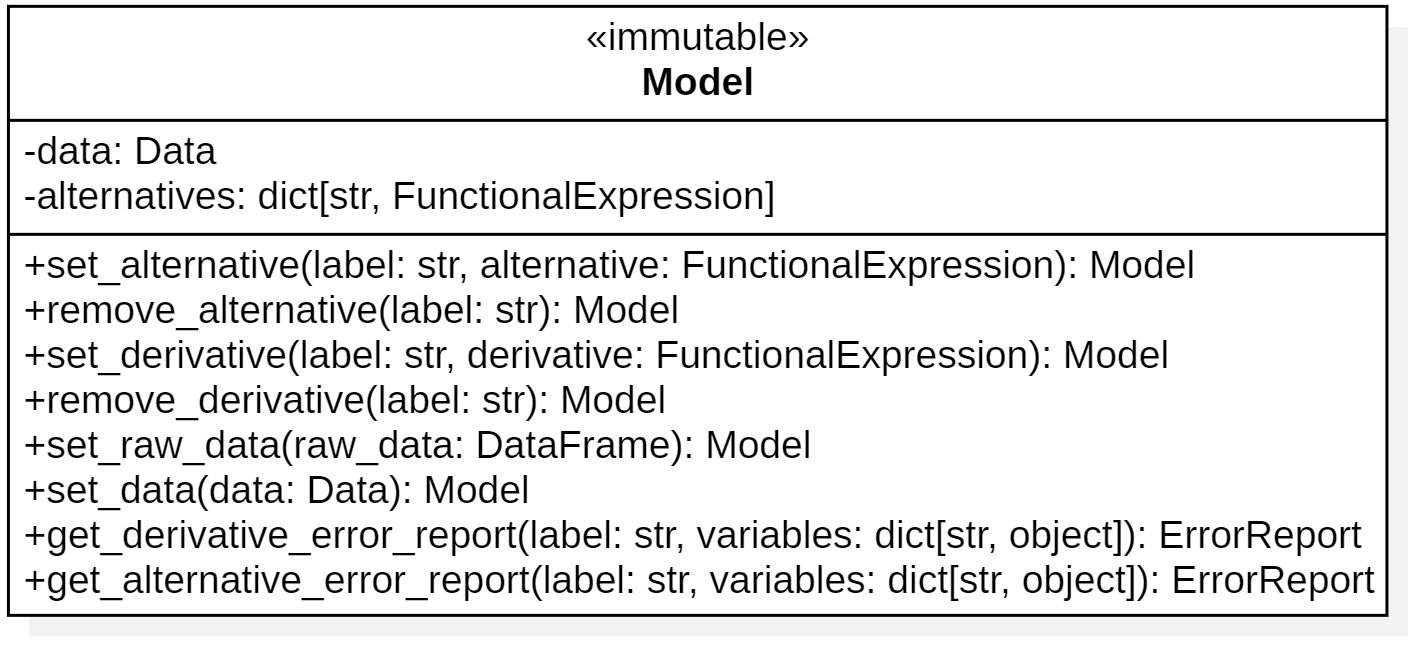
\includegraphics[width=13cm]{entwurf/Entwurf_dokument/img/cls/model/Model.png}
    \caption{Klassendiagramm \texttt{Model}}
\end{figure}

Verwaltet die Daten, die das Modell definieren und wird als Eingabe der Berechnung verwendet. Die Klasse ist die Schnittstelle bei Abfragen und Änderungen des Modells.\\
Die Klasse nimmt Bezug auf \texttt{DataFrame} aus dem externen Paket \texttt{pandas} um die importierten Rohdaten des Nutzers zu speichern.
\newline \newline

\textbf{{Attribute}}
\begin{itemize}
\item \texttt{alternatives: dict[label: str, expr: FunctionalExpression]} \newline
Definierte Alternativen mit eindeutigem Bezeichner.
\item \texttt{data: Data} \newline In das Projekt importierte Erhebungsdaten und Schnittstelle zur Verwaltung der Ableitungen.
\\\\
\end{itemize}

\textbf{{Methoden}}
\begin{itemize}
\item \texttt{set\char`_alternative(label: str, alternative: FunctionalExpression): Model} \newline Hinzufügen oder Ändern einer Alternative. Das \texttt{Model}-Objekt wird dabei nicht verändert, sondern gibt eine Kopie mit der Veränderung zurück.
\\\\
\underline{{Parameter}}

\begin{tabular}{lll}
 & \texttt{label} & Eindeutiger Bezeichner der Alternative. \\
 & \texttt{alternative} & Funktionaler Ausdruck der Alternative. \\
\end{tabular}

\underline{{Rückgabewert}}

\begin{tabular}{lll}
 & \texttt{:Model} & \texttt{Model} nach Veränderung der Alternative. \\
\end{tabular}

\underline{Exceptions}\\
\begin{tabular}{lll}
 & \texttt{ValueError} & Bezeichner der Alternative ist ungültig.\\
\end{tabular}


\item \texttt{remove\char`_alternative(label: str): Model} \newline Entfernen einer existierenden Alternative. \texttt{Model} wird dabei nicht verändert, sondern gibt eine Kopie mit der Veränderung zurück.
\\\\
\underline{{Parameter}}

\begin{tabular}{lll}
 & \texttt{label} & Eindeutiger Bezeichner der Alternative. \\
\end{tabular}

\underline{{Rückgabewert}}

\begin{tabular}{lll}
 & \texttt{:Model} & \texttt{Model} nach Entfernen der Alternative. \\
\end{tabular}

\underline{Exceptions}\\
\begin{tabular}{lll}
 & \texttt{ValueError} & Bezeichner der Alternative ist ungültig.\\
\end{tabular}


\item \texttt{set\char`_derivative(label: str, derivative: FunctionalExpression): Model} \newline Hinzufügen oder Ändern einer Ableitung im assoziierten \texttt{Data}-Objekt. Das \texttt{Model}-Objekt wird dabei nicht verändert, sondern gibt eine Kopie mit der Veränderung zurück.
\\\\
\underline{{Parameter}}

\begin{tabular}{lll}
 & \texttt{label} & Eindeutiger Bezeichner der Ableitung. \\
 & \texttt{derivative} & Ausdruck der Ableitung. \\
\end{tabular}

\underline{{Rückgabewert}}

\begin{tabular}{lll}
 & \texttt{:Model} & \texttt{Model} nach Veränderung der Ableitung. \\
\end{tabular}

\underline{Exceptions}\\
\begin{tabular}{lll}
 & \texttt{ValueError} & Ableitungsbezeichner ist ungültig.\\
\end{tabular}


\item \texttt{remove\char`_derivative(label: str): Model} \newline Entfernen einer existierenden Ableitung im assoziierten \texttt{Data}-Objekt. Das \texttt{Model}-Objekt wird dabei nicht verändert, sondern gibt eine Kopie mit der Veränderung zurück.
\\\\
\underline{{Parameter}}

\begin{tabular}{lll}
 & \texttt{label} & Eindeutiger Bezeichner der Ableitung. \\
\end{tabular}

\underline{{Rückgabewert}}

\begin{tabular}{lll}
 & \texttt{:Model} & \texttt{Model} nach Entfernen der Ableitung. \\
\end{tabular}

\underline{Exceptions}\\
\begin{tabular}{lll}
 & \texttt{ValueError} & Ableitungsbezeichner ist ungültig.\\
\end{tabular}


\item \texttt{set\char`_raw\char`_data(raw\char`_data: DataFrame): Model} \newline Verändern der Erhebungsdaten im assoziierten \texttt{Data}-Objekt. Das \texttt{Model}-Objekt wird dabei nicht verändert, sondern gibt eine Kopie mit der Veränderung zurück.
\\\\
\underline{{Parameter}}

\begin{tabular}{lll}
 & \texttt{raw\char`_data} & Importierte Rohdaten für das Modell. \\
\end{tabular}

\underline{{Rückgabewert}}

\begin{tabular}{lll}
 & \texttt{:Model} & \texttt{Model} nach Veränderung der Rohdaten. \\
\end{tabular}


\item \texttt{set\char`_data(data: Data): Model} \newline Verändern der Erhebungsdaten oder der Ableitungen. Das \texttt{Model}-Objekt wird dabei nicht verändert, sondern gibt eine Kopie mit der Veränderung zurück.
\\\\
\underline{{Parameter}}

\begin{tabular}{lll}
 & \texttt{data} & Neues \texttt{Data}-Objekt mit angewandter Veränderung. \\
\end{tabular}

\underline{{Rückgabewert}}

\begin{tabular}{lll}
 & \texttt{:Model} & \texttt{Model} nach Veränderung des \texttt{Data}-Objekts. \\
\end{tabular}


\item \texttt{get\char`_derivative\char`_error\char`_report(label: str, variables: dict[str, object]): ErrorReport} \newline Beschreibung
\\\\
\underline{{Parameter}}

\begin{tabular}{lll}
 & \texttt{label} & Eindeutiger Bezeichner der Ableitung.  \\
 & \texttt{variables} & Beschreibung \\
\end{tabular}

\underline{{Rückgabewert}}

\begin{tabular}{lll}
 & \texttt{:ErrorReport} & Beschreibung \\
\end{tabular}

\underline{Exceptions}\\
\begin{tabular}{lll}
 & \texttt{ValueError} & Ableitungsbezeichner ist ungültig.\\
\end{tabular}



\item \texttt{get\char`_alternative\char`_error\char`_report(label: str, variables: dict[str, object]): ErrorReport} \newline Beschreibung
\\\\
\underline{{Parameter}}

\begin{tabular}{lll}
 & \texttt{label} & Eindeutiger Bezeichner der Alternative. \\
 & \texttt{variables} & Beschreibung \\
\end{tabular}

\underline{{Rückgabewert}}

\begin{tabular}{lll}
 & \texttt{:ErrorReport} & Beschreibung \\
\end{tabular}

\underline{Exceptions}\\
\begin{tabular}{lll}
 & \texttt{ValueError} & Bezeichner der Alternative ist ungültig.\\
\end{tabular}
\end{itemize}

\newpage
\textbf{\large{Data}}\\\\
\textit{\flqq{}immutable\frqq}\normalsize\\\\
\begin{figure}[H]%
    \centering
    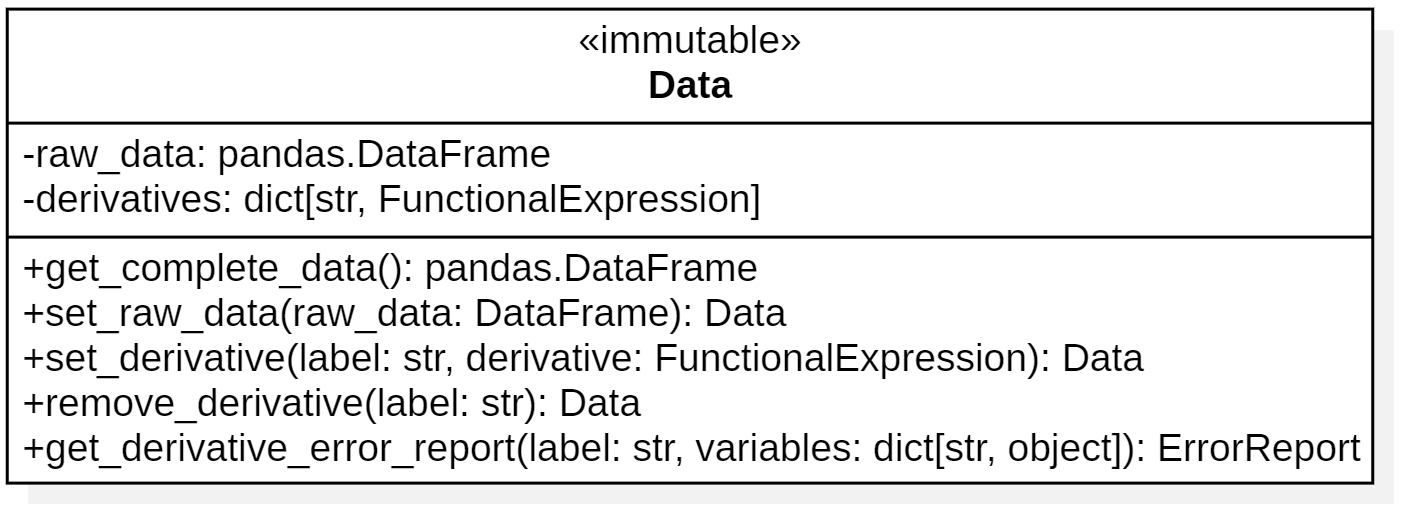
\includegraphics[width=13cm]{entwurf/Entwurf_dokument/img/cls/model/Data.png}
    \caption{Klassendiagramm \texttt{Data}}
\end{figure}

Verwaltet die Daten der importierten Erhebungsdaten und der Ableitungen. Abfragen und Änderungen werden über die Klasse \texttt{Model} aufgerufen.\\
Die Klasse nimmt Bezug auf \texttt{DataFrame} aus dem externen Paket \texttt{pandas} um die importierten Rohdaten des Nutzers zu speichern.
\newline \newline

\textbf{{Attribute}}
\begin{itemize}
\item \texttt{raw\char`_data: DataFrame} \newline Importierte Erhebungsdaten.
\item \texttt{derivatives: dict[label: str, expr: FunctionalExpression]} \newline Definierte Ableitungen mit eindeutigem Bezeichner.
\\\\
\end{itemize}

\textbf{{Methoden}}
\begin{itemize}
\item \texttt{get\char`_complete\char`_data(): DataFrame} \newline Erzeugt ein neues \texttt{DataFrame}, das die Rohdaten und die berechneten Ableitungen zusammensetzt.
\\\\
\underline{{Rückgabewert}}

\begin{tabular}{lll}
 & \texttt{DataFrame} & Zusammensetzung der Rohdaten mit den berechneten Ableitungen. \\
\end{tabular}

\item \texttt{set\char`_raw\char`_data(raw\char`_data: DataFrame): Data} \newline Verändern der Rohdaten. \texttt{Data} wird dabei nicht verändert, sondern gibt eine Kopie mit der Veränderung zurück.
\\\\
\underline{{Parameter}}

\begin{tabular}{lll} 
 & \texttt{raw\char`_data} & Importierte Rohdaten für das Modell. \\
\end{tabular}

\underline{{Rückgabewert}}

\begin{tabular}{lll}
 & \texttt{:Data} & \texttt{Data} nach Veränderung der Rohdaten.  \\
\end{tabular}

\item \texttt{set\char`_derivative(label: str, derivative: FunctionalExpression): Data} \newline Hinzufügen oder Ändern einer Ableitung. Das \texttt{Data}-Objekt wird dabei nicht verändert, sondern gibt eine Kopie mit der Veränderung zurück.
\\\\
\underline{{Parameter}}

\begin{tabular}{lll}
 & \texttt{label} & Eindeutiger Bezeichner der Ableitung. \\
 & \texttt{derivative} & Ausdruck der Ableitung. \\
\end{tabular}

\underline{{Rückgabewert}}

\begin{tabular}{lll}
 & \texttt{:Data} & \texttt{Data} nach Veränderung der Ableitung. \\
\end{tabular}

\underline{Exceptions}\\
\begin{tabular}{lll}
 & \texttt{ValueError} & Ableitungsbezeichner ist ungültig.\\
\end{tabular}


\item \texttt{remove\char`_derivative(label: str): Data} \newline Entfernen einer existierenden Ableitung. Das \texttt{Data}-Objekt wird dabei nicht verändert, sondern gibt eine Kopie mit der Veränderung zurück.
\\\\
\underline{{Parameter}}

\begin{tabular}{lll}
 & \texttt{label} & Eindeutiger Bezeichner der Ableitung. \\
\end{tabular}

\underline{{Rückgabewert}}

\begin{tabular}{lll}
 & \texttt{:Data} & \texttt{Data} nach Entfernen der Ableitung. \\
\end{tabular}

\underline{Exceptions}\\
\begin{tabular}{lll}
 & \texttt{ValueError} & Ableitungsbezeichner ist ungültig.\\
\end{tabular}

\item \texttt{get\char`_derivative\char`_error\char`_report(label: str, variables: dict[str, object]): ErrorReport} \newline Beschreibung
\\\\
\underline{{Parameter}}

\begin{tabular}{lll}
 & \texttt{label} & Eindeutiger Bezeichner der Ableitung. \\
 & \texttt{variables} & Beschreibung \\
\end{tabular}

\underline{{Rückgabewert}}

\begin{tabular}{lll}
 & \texttt{:ErrorReport} & Beschreibung \\
\end{tabular}

\underline{Exceptions}\\
\begin{tabular}{lll}
 & \texttt{ValueError} & Ableitungsbezeichner ist ungültig.\\
\end{tabular}
\end{itemize}

\newpage
\subsubsection{Functions}
\textbf{\large{FunctionalExpression}}\\\\
\textit{\flqq{}immutable\frqq}\normalsize\\\\
\begin{figure}[H]%
    \centering
    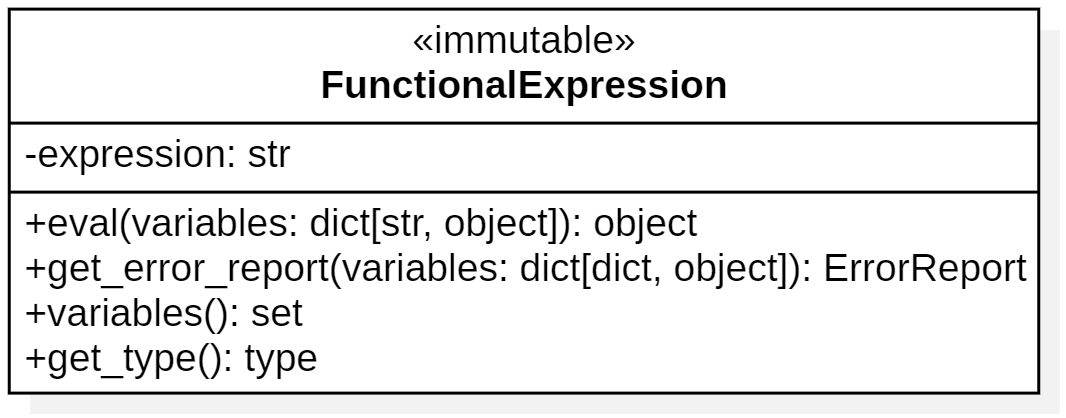
\includegraphics[width=10cm]{entwurf/Entwurf_dokument/img/cls/model/FunctionalExpression.png}
    \caption{Klassendiagramm \texttt{FunctionalExpression}}
\end{figure}

Repräsentation des Funktionsausdrucks einer definierten Attributsableitung oder Alternative.
\newline \newline

\textbf{{Attribute}}
\begin{itemize}
\item \texttt{expression: str} \newline Funktionsausdruck in textueller Form.
\\\\
\end{itemize}

\textbf{{Methoden}}
\begin{itemize}
\item \texttt{eval(variables: dict[str, object])} \newline Evaluiert den gespeicherten Funktionsausdruck.
\\\\
\underline{{Parameter}}

\begin{tabular}{lll}
 & \texttt{variables} & Zuweisungen der Variablen zu den damit definierten Objekten. Diese Variablen können im Ausdruck verwendet werden. \\
\end{tabular}

\underline{{Rückgabewert}}

\begin{tabular}{lll}
 & \texttt{:object} & Berechnetes Ergebnis nach Evaluierung des Ausdrucks. \\
\end{tabular}

\item \texttt{is\char`_valid(): bool} \newline Überprüft, ob der Funktionsausdruck syntaktisch korrekt ist.
\\\\
\underline{{Rückgabewert}}

\begin{tabular}{lll}
 & \texttt{:bool} & \texttt{True}, wenn der Ausdruck syntaktisch korrekt ist. Andernfalls \texttt{False}. \\
\end{tabular}

\item \texttt{variables(): set} \newline Gibt die im Ausruck verwendeten Variablen zurück.
\\\\
\underline{{Rückgabewert}}

\begin{tabular}{lll}
 & \texttt{:set} & Verwendete Variablen im Ausdruck. \\
\end{tabular}

\item \texttt{get\char`_type(): type} \newline Gibt den resultierenden Datentypen nach Evaluierung des Ausdrucks zurück.
\\\\
\underline{{Rückgabewert}}

\begin{tabular}{lll}
 & \texttt{:type} & Datentyp des Ausdrucks. \\
\end{tabular}
\end{itemize}


\newpage
\textbf{\large{Interval}}\\\\
\textit{\flqq{}immutable\frqq}\normalsize\\\\
\begin{figure}[H]%
    \centering
    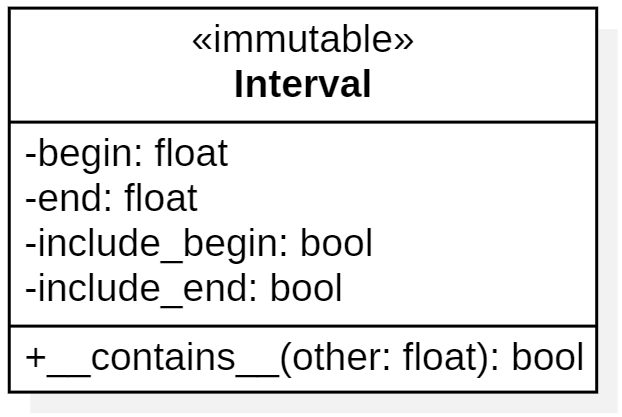
\includegraphics[width=10cm]{entwurf/Entwurf_dokument/img/cls/model/Interval.png}
    \caption{Klassendiagramm \texttt{Interval}}
\end{figure}

Darstellung eines Intervalls. Definierbar bei Festlegung der Ableitungen. Wird bei der Evaluation der Ableitung erzeugt und kann ausgewertet werden.
\newline \newline

\textbf{{Attribute}}
\begin{itemize}
\item \texttt{begin: float} \newline Beginn des Intervalls. \texttt{None} bei fehlender unterer Intervallgrenze. 
\item \texttt{end: float} \newline Ende des Intervalls. \texttt{None} bei fehlender oberer Intervallgrenze. 
\item \texttt{include\char`_begin: bool} \newline Intervall inkludiert den Beginn.
\item \texttt{include\char`_end: bool} \newline Intervall inkludiert das Ende.
\\\\
\end{itemize}

\textbf{{Methoden}}
\begin{itemize}
\item \texttt{\char`_\char`_contains\char`_\char`_(other: float): bool} \newline Überprüft ob ein Wert im Intervall liegt.
\\\\
\underline{{Parameter}}

\begin{tabular}{lll}
 & \texttt{other} & Zu überprüfender Wert. \\
\end{tabular}

\underline{{Rückgabewert}}

\begin{tabular}{lll}
 & \texttt{:bool} & \texttt{True}, falls der Wert im Intervall liegt. Andernfalls \texttt{False}. \\
\end{tabular}
\end{itemize}


\newpage
\textbf{\large{GroupMap}}\\\\
\textit{\flqq{}immutable\frqq}\normalsize\\\\
\begin{figure}[H]%
    \centering
    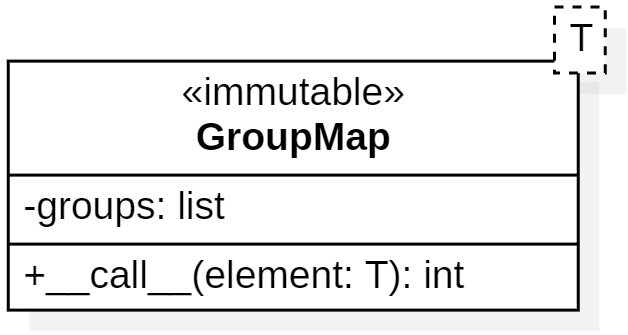
\includegraphics[width=10cm]{entwurf/Entwurf_dokument/img/cls/model/GroupMap.png}
    \caption{Klassendiagramm \texttt{GroupMap}}
\end{figure}

Darstellung einer Liste von Gruppen mit Elementen. Definierbar bei Festlegung der Ableitungen. Wird bei der Evaluation der Ableitung erzeugt und kann ausgewertet werden.
\newline \newline

\textbf{Attribute}
\begin{itemize}
\item \texttt{groups: list} \newline Liste der Gruppen mit Elementen.
\\\\
\end{itemize}

\textbf{Methoden}
\begin{itemize}
\item \texttt{\char`_\char`_call\char`_\char`_(element: T): int} \newline Überprüft in welcher Gruppe sich ein Element befindet und gibt den Index zurück.
\\\\
\underline{{Parameter}}

\begin{tabular}{lll}
 & \texttt{element} & Zu überprüfendes Element. \\
\end{tabular}

\underline{Rückgabewert}

\begin{tabular}{lll}
 & \texttt{:int} & Index der Gruppe, in welcher sich das Element befindet. \\
 && \texttt{-1}, falls in keiner der Gruppen.\\
\end{tabular}
\end{itemize}


\newpage
\textbf{\large{ErrorReport}}\\\\
\textit{\flqq{}immutable\frqq}\normalsize\\\\
\begin{figure}[H]%
    \centering
    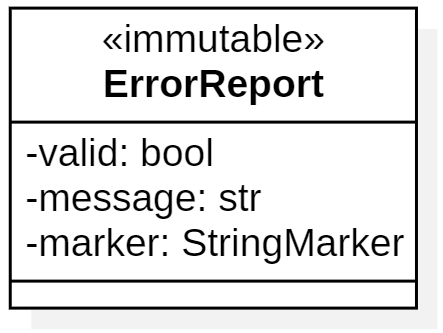
\includegraphics[width=7cm]{entwurf/Entwurf_dokument/img/cls/model/ErrorReport.png}
    \caption{Klassendiagramm \texttt{ErrorReport}}
\end{figure}

Beschreibt Fehlermeldungen in Ausdrücken der \texttt{FunctionalExpression}-Klasse. \\ Ermöglicht eine visuelle Repräsentation der Fehlermeldung am invaliden Ausdruck.
\newline \newline

\textbf{Attribute}
\begin{itemize}
\item \texttt{valid: bool} \newline Beschreibung
\item \texttt{message: str} \newline Angezeigetext der Fehlermeldung.
\item \texttt{marker: StringMarker} \newline Visualisierbare Position des Fehlers.
\\\\
\end{itemize}


\newpage
\textbf{\large{StringMarker}}\\\\
\textit{\flqq{}immutable\frqq}\normalsize\\\\
\begin{figure}[H]%
    \centering
    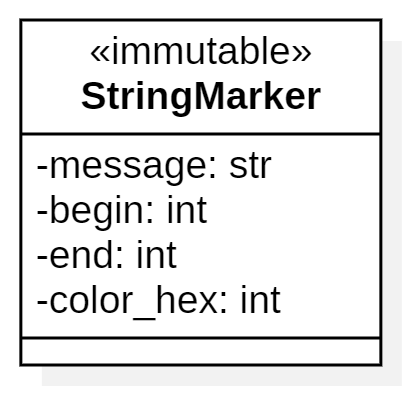
\includegraphics[width=7cm]{entwurf/Entwurf_dokument/img/cls/model/StringMarker.png}
    \caption{Klassendiagramm \texttt{StringMarker}}
\end{figure}

Speichert die Markierung eines Substrings. Wird bei Ferhlermeldung zu einer \texttt{FunctionalExpression} verwendet, um den Fehler eindeutig zu visualisieren.
\newline \newline

\textbf{Attribute}
\begin{itemize}
\item \texttt{begin: int} \newline Beginn des Substrings, auf den sich die Fehlermeldung bezieht.
\item \texttt{end: int} \newline Ende des Substrings, auf den sich die Fehlermeldung bezieht.
\item \texttt{color\char`_hex: int} \newline Farbe der Hervorhebung als RGB kodiert in Hexadezimal.
\\\\
\end{itemize}


\newpage
\subsubsection{Processing}

%----------------------------------
\subsubsection*{\large{\textbf{ProcessingConfig}\label{cls:ProcessingConfig}}}
\textit{\flqq{}abstract\frqq} \textit{\flqq{}immutable\frqq}\normalsize\\\\
\begin{tabular}{lll}
 Superklassen: & --\\
 Subklassen: & \texttt{SimpleProcessingConfig}, \texttt{VariedProcessingConfig}
\end{tabular}\\
\begin{figure}[H]%
    \centering
    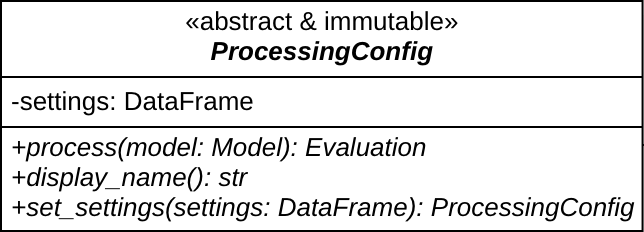
\includegraphics[width=13cm]{entwurf/Entwurf_dokument/img/cls/model/ProcessingConfig.png}
    \caption{Klassendiagramm \texttt{ProcessingConfig}}
\end{figure}

Die Klasse definiert, auf welche Art und Weise eine Datenverarbeitung eines Datenmodells erfolgt.
\\\\

\textbf{Attribute}
\begin{itemize}\setlength\itemsep{3em}
\item \texttt{settings: pandas.DataFrame}\\\\
Datentabelle der Nutzereinstellungen.
\\\\
\end{itemize}

\textbf{Methoden}
\begin{itemize}\setlength\itemsep{3em}
\item \textit{\flqq{}abstract\frqq} \texttt{\textit{process(model: Model): Evaluation}}\\\\
Verarbeitet ein \texttt{model} entsprechend der Konfigurationsklasse und erstellt eine Auswertung vom Typ \texttt{Evaluation}.
\\\\
\underline{Parameter}\\
\begin{tabular}{lll}
 & \texttt{model} & Diskretes Wahlmodell, auf dem eine Verabreitung erfolgen soll.\\
\end{tabular}

\underline{Rückgabewert}\\
\begin{tabular}{lll}
 & Auswertung, wie durch Konfigurationsklasse definiert.\\
\end{tabular}

\underline{Exceptions}\\
\begin{tabular}{lll}
 & \texttt{ValueError} & Modell hat nicht die durch die Konfiguration geforderten Eigenschaften.\\
\end{tabular}

\item \textit{\flqq{}abstract\frqq} \texttt{\textit{display\char`_name(): str}}\\\\
Getter für Anzeigename der Konfigurationsklasse zur Darstellung im Auswahlmenü.
\\\\
\underline{Rückgabewert}\\
\begin{tabular}{lll}
 & Anzeigename als \texttt{str}.\\
\end{tabular}

\item \textit{\flqq{}abstract\frqq} \texttt{\textit{set\char`_settings(settings: pandas.DataFrame): ProcessingConfig}}\\\\
Erstellt eine Kopie des Objekts, in der lediglich das Attribut \texttt{settings} durch das übergebene Attribut überschrieben wird.
\\\\
\underline{Parameter}\\
\begin{tabular}{lll}
 & \texttt{settings} & Neue Datentabelle der Nutzereinstellungen.\\
\end{tabular}

\underline{Rückgabewert}\\
\begin{tabular}{lll}
 & Anzeigename als \texttt{str}.\\
\end{tabular}
\end{itemize}

%----------------------------------
\newpage
\subsubsection*{\large{\textbf{SimpleProcessingConfig}\label{cls:SimpleProcessingConfig}}}
\textit{\flqq{}immutable\frqq}\normalsize\\\\
\begin{tabular}{lll}
 Superklassen: & \texttt{ProcessingConfig}\\
 Subklassen: & --
\end{tabular}\\
\begin{figure}[H]%
    \centering
    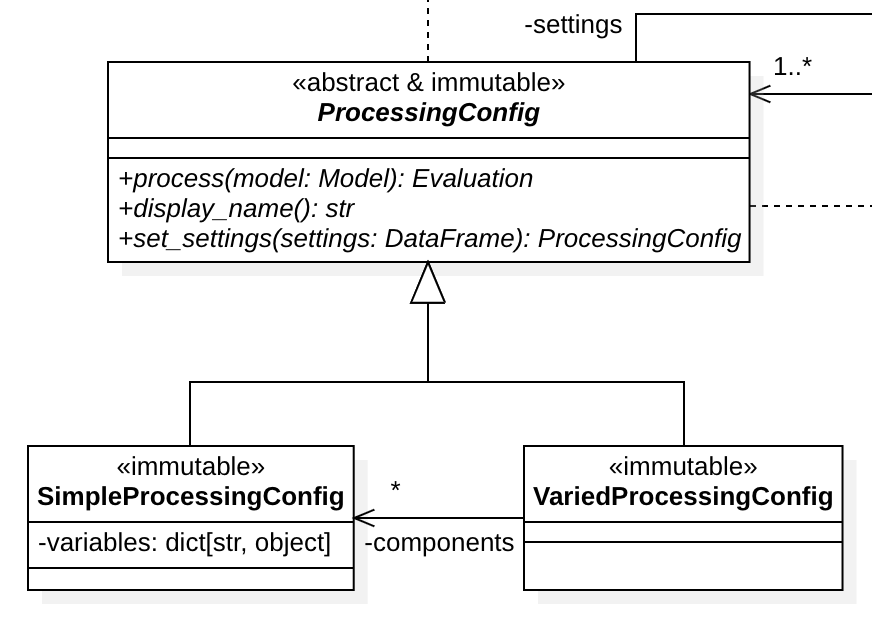
\includegraphics[width=13cm]{entwurf/Entwurf_dokument/img/cls/model/ProcessingConfigs.png}
    \caption{Klassendiagramm aller Subklassen von \texttt{ProcessingConfig}}
\end{figure}

Die Klasse definiert das Verfahren einer einfachen Parameterschätzung eines diskreten Wahlmodells und weist den verbleibenden freie Variablen im Modell einen Wert zu.
\\\\

\textbf{Attribute}
\begin{itemize}\setlength\itemsep{3em}
\item \texttt{variables: dict[str, object]}\\\\
Zuordnung zwischen verbleibenden freien Variablen und einem Wert, der für die Berechnung verwendet werden soll.\\
Der Datentyp der Werte kann nicht weiter eingeschränkt werden, da dieser von der Verwendung der freien Variablen abhängt.
\\\\
\end{itemize}

\textbf{Methoden}
\begin{itemize}\setlength\itemsep{3em}
\item \texttt{process(model: Model): Evaluation}\\\\
Wendet die definierte Parameterschätzung auf \texttt{model} an und erstellt eine Auswertung vom Typ \texttt{Evaluation}.
\\\\
\underline{Parameter}\\
\begin{tabular}{lll}
 & \texttt{model} & Diskretes Wahlmodell, auf dem eine Verarbeitung erfolgen soll.\\
\end{tabular}

\underline{Rückgabewert}\\
\begin{tabular}{lll}
 & Auswertung, wie durch Konfigurationsklasse definiert.\\
\end{tabular}

\underline{Exceptions}\\
\begin{tabular}{lll}
 & \texttt{ValueError} & Modell hat nicht die durch die Konfiguration geforderten Eigenschaften.\\
\end{tabular}
\end{itemize}

%----------------------------------
\newpage
\subsubsection*{\large{\textbf{VariedProcessingConfig}\label{cls:VariedProcessingConfig}}}
\textit{\flqq{}immutable\frqq}\normalsize\\\\
\begin{tabular}{lll}
 Superklassen: & \texttt{ProcessingConfig}\\
 Subklassen: & --
\end{tabular}\\
\begin{figure}[H]%
    \centering
    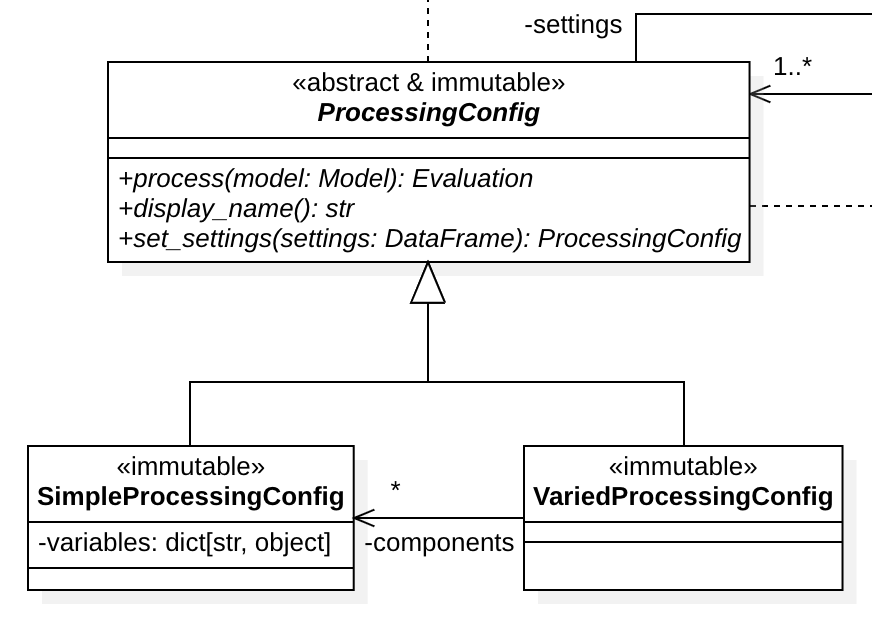
\includegraphics[width=13cm]{entwurf/Entwurf_dokument/img/cls/model/ProcessingConfigs.png}
    \caption{Klassendiagramm aller Subklassen von \texttt{ProcessingConfig}}
\end{figure}

Die Klasse definiert eine mehrfache Anwendung einer Parameterschätzung eines diskreten Wahlmodells und weist dabei den verbleibenden freie Variablen im Modell je unterschiedliche Werte zu. Die Werte können definiert werden und müssen vor dem Aufruf von \texttt{process} vorliegen.
\\\\

\textbf{Attribute}
\begin{itemize}\setlength\itemsep{3em}
\item \texttt{components: list[SimpleProcessingConfig]}\\\\
Liste von Konfigurationen vom Typ \texttt{SimpleProcessingConfig}, die nacheinander ausgeführt werden sollen.
\\\\
\end{itemize}

\textbf{Methoden}
\begin{itemize}\setlength\itemsep{3em}
\item \texttt{process(model: Model): Evaluation}\\\\
Wendet alle hinterlegten einzelnen Parameterschätzungen auf \texttt{model} an und erstellt eine Auswertung vom Typ \texttt{Evaluation}.
\\\\
\underline{Parameter}\\
\begin{tabular}{lll}
 & \texttt{model} & Diskretes Wahlmodell, auf dem eine Verabreitung erfolgen soll.\\
\end{tabular}

\underline{Rückgabewert}\\
\begin{tabular}{lll}
 & Auswertung, wie durch Konfigurationsklasse definiert.\\
\end{tabular}

\underline{Exceptions}\\
\begin{tabular}{lll}
 & \texttt{ValueError} & Modell hat nicht die durch die Konfiguration geforderten Eigenschaften.\\
\end{tabular}
\end{itemize}

%----------------------------------
\newpage
\subsubsection*{\large{\textbf{Evaluation}\label{cls:Evaluation}}}
\textit{\flqq{}immutable\frqq}\normalsize\\\\
\begin{tabular}{lll}
 Superklassen: & --\\
 Subklassen: & --
\end{tabular}\\
\begin{figure}[H]%
    \centering
    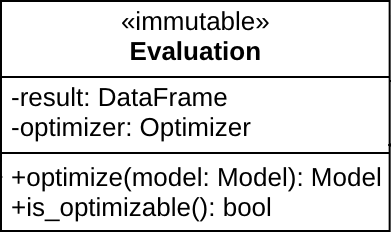
\includegraphics[width=13cm]{entwurf/Entwurf_dokument/img/cls/model/Evaluation.png}
    \caption{Klassendiagramm von \texttt{Evaluation}}
\end{figure}

Die Klasse entspricht der Auswertung einer Parameterschätzung von einem diskreten Wahlmodell.
\\\\

\textbf{Attribute}
\begin{itemize}\setlength\itemsep{3em}
\item \texttt{result: pandas.DataFrame}\\\\
Auswertungstabelle der verwendeten Berechnungsbibliothek oder eine zusammengesetzte Tabelle aus mehreren Auswertungstabellen.
\\\\
\end{itemize}

\textbf{Methoden}
\begin{itemize}\setlength\itemsep{3em}
\item \texttt{optimize(model: Model): Model}\\\\
Falls der Auswertung ein Modelloptimierungsverfahren beiliegt (siehe \texttt{is\char`_optimizable()}), wird das diskrete Wahlmodell dementsprechend verbessert.\\\\
\underline{Parameter}\\
\begin{tabular}{lll}
 & \texttt{model} & Diskretes Wahlmodell, das optimiert werden soll.\\
\end{tabular}

\underline{Rückgabewert}\\
\begin{tabular}{lll}
 & Das optimierte diskrete Wahlmodell.\\
\end{tabular}

\underline{Exceptions}\\
\begin{tabular}{lll}
 & \texttt{ValueError} & Modell hat nicht die durch den Optimierungsalgorithmus\\
 && geforderten Eigenschaften.\\
\end{tabular}

\item \texttt{is\char`_optimizable(): bool}\\\\
Prüft, ob eine Optimierung auf Grundlage dieser Auswertung prinzipiell möglich ist.\\\\
\underline{Parameter}\\
\begin{tabular}{lll}
 & Keine Parameter.
\end{tabular}

\underline{Rückgabewert}\\
\begin{tabular}{lll}
 & Wahrheitswert, ob Optimierung auf Grundlage dieser Auswertung prinzipiell möglich ist.\\
\end{tabular}
\end{itemize}


%----------------------------------
\newpage
\subsubsection*{\large{\textbf{Optimizer}\label{cls:Optimizer}}}
\textit{\flqq{}interface\frqq}\normalsize\\\\
\begin{tabular}{lll}
 Superklassen: & --\\
 Subklassen: & --
\end{tabular}\\
\begin{figure}[H]%
    \centering
    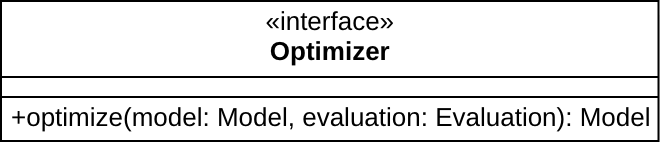
\includegraphics[width=13cm]{entwurf/Entwurf_dokument/img/cls/model/Optimizer.png}
    \caption{Klassendiagramm von \texttt{Optimizer}}
\end{figure}

Das Interface bietet eine Schnittstelle zur Implementierung eines Optimierungsalgorithmus.
\\\\

\textbf{Methoden}
\begin{itemize}\setlength\itemsep{3em}
\item \textit{\flqq{}abstract\frqq} \texttt{\textit{optimize(model: Model, evaluation: Evaluation): Model}}\\\\
Falls der Auswertung ein Modelloptimierungsverfahren beiliegt (siehe \texttt{is\char`_optimizable()}), wird das diskrete Wahlmodell dementsprechend verbessert.\\\\
\underline{Parameter}\\
\begin{tabular}{lll}
 & \texttt{model} & Diskretes Wahlmodell, das optimiert werden soll.\\
 & \texttt{evaluation} & Auswertung, auf deren Grundlage eine Optimierung vorgenommen werden soll.
\end{tabular}

\underline{Rückgabewert}\\
\begin{tabular}{lll}
 & Das optimierte diskrete Wahlmodell.\\
\end{tabular}

\underline{Exceptions}\\
\begin{tabular}{lll}
 & \texttt{ValueError} & Ein Parameter hat nicht die durch den Optimierungsalgorithmus\\
 && geforderten Eigenschaften.\\
\end{tabular}
\end{itemize}


%----------------------------------
\newpage
\subsubsection*{\large{\textbf{Project}\label{cls:Project}}}
\textit{\flqq{}interface\frqq}\normalsize\\\\
\begin{tabular}{lll}
 Superklassen: & \texttt{ProcessingConfig}\\
 Subklassen: & --
\end{tabular}\\
\begin{figure}[H]%
    \centering
    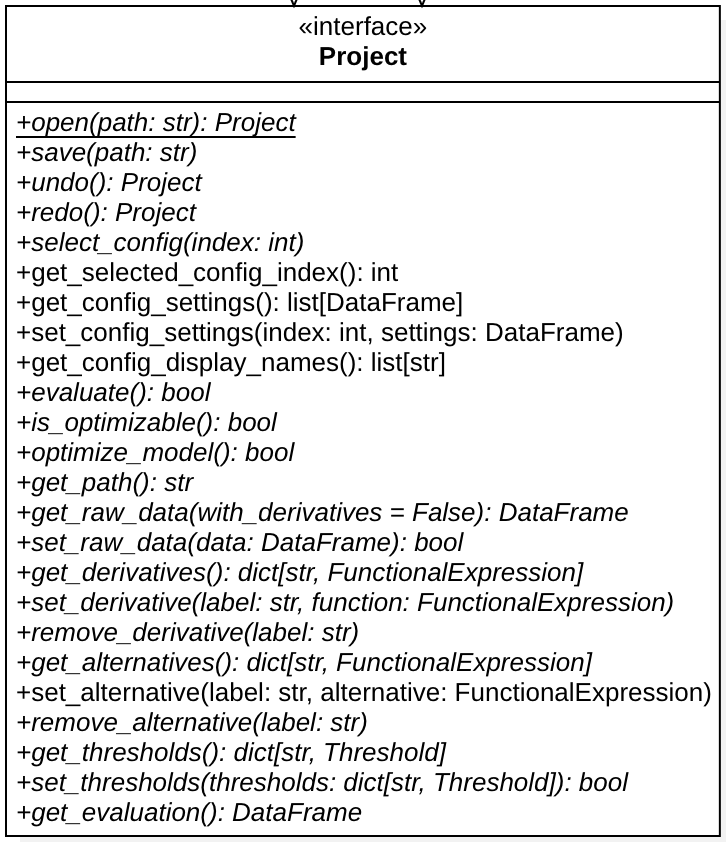
\includegraphics[width=13cm]{entwurf/Entwurf_dokument/img/cls/model/Project.png}
    \caption{Klassendiagramm von \texttt{Project}}
\end{figure}

Das Interface stellt die Schnittstelle zwischen Datenmodell (\emph{Model}) und Benutzeroberfläche (\emph{View} und \emph{Controller}) dar. Es beinhaltet alle benötigten Methoden zur vollständigen Verwaltung eines Projekts.
\\\\

\textbf{Methoden}
\begin{itemize}\setlength\itemsep{3em}
\item \textit{\flqq{}static\frqq} \texttt{\underline{open(path: str): Project}}\\\\
Lädt ein unter \texttt{path} gespeichertes Projekt.
\\\\
\underline{Parameter}\\
\begin{tabular}{lll}
 & \texttt{path} & Dateipfad des Projekts.\\
\end{tabular}

\underline{Rückgabewert}\\
\begin{tabular}{lll}
 & Interface des Projekts.\\
\end{tabular}

\underline{Exceptions}\\
\begin{tabular}{lll}
 & \texttt{ValueError} & Dateipfad ist ungültig.\\
 & \texttt{IOError} & Fehler bei I/O-Operation.\\
\end{tabular}


\item \textit{\flqq{}abstract\frqq} \texttt{\textit{save(path: str = None)}}\\\\
Speichert ein Projekt unter \texttt{path}.
\\\\
\underline{Parameter}\\
\begin{tabular}{lll}
 & \texttt{path} & Dateipfad des Projekts.\\
 && Standardmäßig auf \texttt{None}.\\
 && Falls Pfad \texttt{None} ist, wird der im Projekt hinterlegte Projektpfad verwendet.\\
\end{tabular}

\underline{Rückgabewert}\\
\begin{tabular}{lll}
 & Keine Rückgabe.\\
\end{tabular}

\underline{Exceptions}\\
\begin{tabular}{lll}
 & \texttt{ValueError} & Dateipfad ist ungültig.\\
 & \texttt{IOError} & Fehler bei I/O-Operation.\\
\end{tabular}


\item \textit{\flqq{}abstract\frqq} \texttt{\textit{undo(): Project}}\\\\
Macht die letzte Änderung am Projekt rückgängig und gibt die letzte Version zurück.
\\\\
\underline{Parameter}\\
\begin{tabular}{lll}
 & Keine Parameter.
\end{tabular}

\underline{Rückgabewert}\\
\begin{tabular}{lll}
 & Projekt-Interface des Projekts vor der zuletzt vor genommenen Operation.\\
\end{tabular}

\underline{Exceptions}\\
\begin{tabular}{lll}
 & \texttt{IndexError} & Keine Vorgängerversion hinterlegt.\\
\end{tabular}


\item \textit{\flqq{}abstract\frqq} \texttt{\textit{redo(): Project}}\\\\
Macht das letzte \texttt{undo()} rückgängig, sofern seitdem nichts am Projekt verändert wurde.
\\\\
\underline{Parameter}\\
\begin{tabular}{lll}
 & Keine Parameter.
\end{tabular}

\underline{Rückgabewert}\\
\begin{tabular}{lll}
 & Projekt-Interface des Projekts vor dem letzten \texttt{undo()}-Aufruf.\\
\end{tabular}

\underline{Exceptions}\\
\begin{tabular}{lll}
 & \texttt{IndexError} & Keine Nachfolgerversion hinterlegt.\\
\end{tabular}


\item \textit{\flqq{}abstract\frqq} \texttt{\textit{select\char`_config(index: int)}}\\\\
Wählt die Konfiguration mit dem Index \texttt{index} aus der im Projekt hinterlegten Liste an Verarbeitungskonfigurationen (\texttt{ProcessingConfig}) für eine spätere Verarbeitung aus.
\\\\
\underline{Parameter}\\
\begin{tabular}{lll}
 & \texttt{index} & Index der gewünschten Konfiguration in der im Projekt hinterlegten Liste.
\end{tabular}

\underline{Rückgabewert}\\
\begin{tabular}{lll}
 & Keine Rückgabe.\\
\end{tabular}

\underline{Exceptions}\\
\begin{tabular}{lll}
 & \texttt{IndexError} & Index existiert nicht.\\
\end{tabular}

\item \textit{\flqq{}abstract\frqq} \texttt{\textit{select\char`_config(index: int)}}\\\\
Wählt die Konfiguration mit dem Index \texttt{index} aus der im Projekt hinterlegten Liste an Verarbeitungskonfigurationen (\texttt{ProcessingConfig}) für eine spätere Verarbeitung aus.
\\\\
\underline{Parameter}\\
\begin{tabular}{lll}
 & \texttt{index} & Index der gewünschten Konfiguration in der im Projekt hinterlegten Liste.
\end{tabular}

\underline{Rückgabewert}\\
\begin{tabular}{lll}
 & Keine Rückgabe.\\
\end{tabular}

\underline{Exceptions}\\
\begin{tabular}{lll}
 & \texttt{IndexError} & Index existiert nicht.\\
\end{tabular}


\item \textit{\flqq{}abstract\frqq} \texttt{\textit{get\char`_selected\char`_config\char`_index(): int}}\\\\
Getter für Index der gewählten Konfiguration aus der im Projekt hinterlegten Liste an Verarbeitungskonfigurationen (\texttt{ProcessingConfig}).
\\\\
\underline{Parameter}\\
\begin{tabular}{lll}
 & Keine Parameter.
\end{tabular}

\underline{Rückgabewert}\\
\begin{tabular}{lll}
 & Index der gewählten Konfiguration.\\
\end{tabular}


\item \textit{\flqq{}abstract\frqq} \texttt{\textit{get\char`_config\char`_settings(): list[pandas.DataFrame]}}\\\\
Getter für eine Liste aller im Projekt hinterlegten Einstellungen von Verarbeitungskonfigurationen (\texttt{ProcessingConfig.settings}).
\\\\
\underline{Parameter}\\
\begin{tabular}{lll}
 & Keine Parameter.
\end{tabular}

\underline{Rückgabewert}\\
\begin{tabular}{lll}
 & Liste aller hinterlegten Einstellungen von Verarbeitungskonfigurationen.\\
 & (\texttt{ProcessingConfig.settings}).\\
\end{tabular}


\item \textit{\flqq{}abstract\frqq} \texttt{\textit{get\char`_config\char`_settings(): list[pandas.DataFrame]}}\\\\
Getter für eine Liste aller im Projekt hinterlegten Einstellungen von Verarbeitungskonfigurationen (\texttt{ProcessingConfig.settings}).
\\\\
\underline{Parameter}\\
\begin{tabular}{lll}
 & Keine Parameter.
\end{tabular}

\underline{Rückgabewert}\\
\begin{tabular}{lll}
 & Liste aller hinterlegten Einstellungen von Verarbeitungskonfigurationen\\
 & (\texttt{ProcessingConfig.settings}).\\
 & Das Orginalobjekt kann über den Rückgabewert nicht modifiziert werden.\\
\end{tabular}


\item \textit{\flqq{}abstract\frqq} \texttt{\textit{set\char`_config\char`_settings\char`_index(index: int, settings: pandas.DataFrame)}}\\\\
Setter für Einstellungen von im Projekt hinterlegten Verarbeitungskonfigurationen (\texttt{ProcessingConfig}).
\\\\
\underline{Parameter}\\
\begin{tabular}{lll}
 & \texttt{index} & Index der Verarbeitungskonfiguration,\\
 && zu der die Einstellungen geändert werden sollen.\\
 & \texttt{settings} & Neue zu setzenden Einstellungen\\
\end{tabular}

\underline{Rückgabewert}\\
\begin{tabular}{lll}
 & Index der gewählten Konfiguration.\\
\end{tabular}


\item \textit{\flqq{}abstract\frqq} \texttt{\textit{get\char`_config\char`_display\char`_names(): list[str]}}\\\\
Getter für eine Liste der Anzeigenamen von allen im Projekt hinterlegten Verarbeitungskonfigurationen (\texttt{ProcessingConfig}).
\\\\
\underline{Parameter}\\
\begin{tabular}{lll}
 & Keine Parameter.
\end{tabular}

\underline{Rückgabewert}\\
\begin{tabular}{lll}
 & Liste der Anzeigenamen.\\
 & Das Orginalobjekt kann über den Rückgabewert nicht modifiziert werden.\\
\end{tabular}


\item \textit{\flqq{}abstract\frqq} \texttt{\textit{evaluate(): bool}}\\\\
Führt das im Projekt konfigurierte Verarbeitungsverfahren aus.
\\\\
\underline{Parameter}\\
\begin{tabular}{lll}
 & Keine Parameter.\\
\end{tabular}

\underline{Rückgabewert}\\
\begin{tabular}{lll}
 & Wahrheitswert, ob Auswertung erfolgreich war.\\
\end{tabular}

\underline{Exceptions}\\
\begin{tabular}{lll}
 & \texttt{ValueError} & Voraussetzungen für eine Berechnung sind nicht erfüllt.\\
\end{tabular}


\item \textit{\flqq{}abstract\frqq} \texttt{\textit{is\char`_optimizable(): bool}}\\\\
Prüft, ob zurzeit eine Modelloptimierung prinzipiell möglich ist.\\\\
\underline{Parameter}\\
\begin{tabular}{lll}
 & Keine Parameter.
\end{tabular}

\underline{Rückgabewert}\\
\begin{tabular}{lll}
 & Wahrheitswert, ob Optimierung prinzipiell möglich ist.\\
\end{tabular}


\item \textit{\flqq{}abstract\frqq} \texttt{\textit{optimize\char`_model(): bool}}\\\\
Führt eine Modelloptimierung auf Grundlage einer zuvor angefertigten Auswertung aus.
\\\\
\underline{Parameter}\\
\begin{tabular}{lll}
 & Keine Parameter.\\
\end{tabular}

\underline{Rückgabewert}\\
\begin{tabular}{lll}
 & Wahrheitswert, ob Optimierung erfolgreich war.\\
\end{tabular}

\underline{Exceptions}\\
\begin{tabular}{lll}
 & \texttt{ValueError} & Voraussetzungen für eine Berechnung sind nicht erfüllt.\\
\end{tabular}


\item \textit{\flqq{}abstract\frqq} \texttt{\textit{get\char`_path(): str}}\\\\
Getter für den Projektdateipfad, an dem das Projekt (u.~a. automatisch) gespeichert wird.
\\\\
\underline{Parameter}\\
\begin{tabular}{lll}
 & Keine Parameter.
\end{tabular}

\underline{Rückgabewert}\\
\begin{tabular}{lll}
 & Projektdateipfad.\\
\end{tabular}


\item \textit{\flqq{}abstract\frqq} \texttt{\textit{get\char`_raw\char`_data(with\char`_derivatives = False): pandas.DataFrame}}\\\\
Getter für eine Liste der im Projekt importierten Rohdaten / Umfragedaten. Bei Bedarf werden auch Spaltenableitungen hinzugefügt.
\\\\
\underline{Parameter}\\
\begin{tabular}{lll}
 & \texttt{with\char`_derivatives} & Gibt an, ob Spaltenableitungen ebenfalls berechnet\\
 && und zur Rückgabe hinzugefügt werden sollen.\\
 && Standardwert ist \texttt{False}.\\
\end{tabular}

\underline{Rückgabewert}\\
\begin{tabular}{lll}
 & Tabelle der Rohdaten.\\
 & Das Orginalobjekt kann über den Rückgabewert nicht modifiziert werden.\\
\end{tabular}

\underline{Exceptions}\\
\begin{tabular}{lll}
 & \texttt{Exception} & Spaltenableitungen konnten nicht korrekt gebildet werden\\
 && (\texttt{with\char`_derivatives = True}).\\
\end{tabular}


\item \textit{\flqq{}abstract\frqq} \texttt{\textit{set\char`_raw\char`_data(data: pandas.DataFrame)}}\\\\
Setter für die im Projekt hinterlegten Rohdaten / Umfragedaten.
\\\\
\underline{Parameter}\\
\begin{tabular}{lll}
 & \texttt{data} & Neuer zu setzender Rohdatensatz.\\
\end{tabular}

\underline{Rückgabewert}\\
\begin{tabular}{lll}
 & Keine Rückgabe.\\
\end{tabular}


\item \textit{\flqq{}abstract\frqq} \texttt{\textit{get\char`_derivatives(): dict[str, FunctionalExpression]}}\\\\
Getter für alle definierten Spaltenableitungsfunktionen.
\\\\
\underline{Parameter}\\
\begin{tabular}{lll}
 & Keine Parameter.\\
\end{tabular}

\underline{Rückgabewert}\\
\begin{tabular}{lll}
 & Dictionary mit Ableitungsbezeichner als Schlüssel und \texttt{FunctionalExpression}\\
 & als zugeordneter Wert.\\
 & Das Orginalobjekt kann über den Rückgabewert nicht modifiziert werden.\\
\end{tabular}


\item \textit{\flqq{}abstract\frqq} \texttt{\textit{set\char`_derivative(label: str, function: FunctionalExpression)}}\\\\
Setter für im Projekt hinterlegte Spaltenableitungen.
\\\\
\underline{Parameter}\\
\begin{tabular}{lll}
 & \texttt{label} & Bezeichner der zu setzende Spaltenableitung.\\
 & \texttt{function} & Ableitungsfunktion als \texttt{FunctionalExpression}.\\
\end{tabular}

\underline{Rückgabewert}\\
\begin{tabular}{lll}
 & Keine Rückgabe.\\
\end{tabular}


\item \textit{\flqq{}abstract\frqq} \texttt{\textit{remove\char`_derivative(label: str)}}\\\\
Setter für im Projekt hinterlegten Spaltenableitungen.
\\\\
\underline{Parameter}\\
\begin{tabular}{lll}
 & \texttt{label} & Bezeichner der zu löschenden Spaltenableitung.\\
\end{tabular}

\underline{Rückgabewert}\\
\begin{tabular}{lll}
 & Keine Rückgabe.\\
\end{tabular}

\underline{Exceptions}\\
\begin{tabular}{lll}
 & \texttt{ValueError} & Ableitungsbezeichner ist ungültig.\\
\end{tabular}


\item \textit{\flqq{}abstract\frqq} \texttt{\textit{import\char`_derivative\char`(path: str)}}\\\\
Importiert eine Spaltenableitungsfunktionen aus einer Datei in das Projekt.
\\\\
\underline{Parameter}\\
\begin{tabular}{lll}
 & \texttt{path} & Dateipfad an dem die Spaltenableitung gespeichert ist.\\
\end{tabular}

\underline{Rückgabewert}\\
\begin{tabular}{lll}
 & Keine Rückgabe.\\
\end{tabular}

\underline{Exceptions}\\
\begin{tabular}{lll}
 & \texttt{ValueError} & Dateipfad ist ungültig.\\
 & \texttt{IOError} & Fehler bei I/O-Operation.\\
\end{tabular}


\item \textit{\flqq{}abstract\frqq} \texttt{\textit{export\char`_derivative(label: str, path: str)}}\\\\
Exportiert eine im Projekt hinterlegte Spaltenableitungsfunktionen.
\\\\
\underline{Parameter}\\
\begin{tabular}{lll}
 & \texttt{label} & Bezeichner der zu exportierenden Spaltenableitung.\\
 & \texttt{path} & Dateipfad an dem die Spaltenableitung gespeichert wird.\\
\end{tabular}

\underline{Rückgabewert}\\
\begin{tabular}{lll}
 & Keine Rückgabe.\\
\end{tabular}

\underline{Exceptions}\\
\begin{tabular}{lll}
 & \texttt{ValueError} & Ableitungsbezeichner oder Dateipfad ist ungültig.\\
 & \texttt{IOError} & Fehler bei I/O-Operation.\\
\end{tabular}


\item \textit{\flqq{}abstract\frqq} \texttt{\textit{get\char`_derivative\char`_error\char`_report(label: str): ErrorReport}}\\\\
Erstellt einen Fehlerbericht zu einer Spaltenableitungsfunktion.
\\\\
\underline{Parameter}\\
\begin{tabular}{lll}
 & \texttt{label} & Bezeichner der zu prüfenden Spaltenableitung.\\
\end{tabular}

\underline{Rückgabewert}\\
\begin{tabular}{lll}
 & Fehlerbericht in Form eines \texttt{ErrorReport}-Objekts.\\
\end{tabular}

\underline{Exceptions}\\
\begin{tabular}{lll}
 & \texttt{ValueError} & Ableitungsbezeichner ist ungültig.\\
\end{tabular}


\item \textit{\flqq{}abstract\frqq} \texttt{\textit{get\char`_alternatives(): dict[str, FunctionalExpression]}}\\\\
Getter für alle definierten Nutzenfunktionen.
\\\\
\underline{Parameter}\\
\begin{tabular}{lll}
 & Keine Parameter.\\
\end{tabular}

\underline{Rückgabewert}\\
\begin{tabular}{lll}
 & Dictionary mit Alternativenbezeichner als Schlüssel und \texttt{FunctionalExpression}\\
 & als zugeordneter Wert.\\
 & Das Orginalobjekt kann über den Rückgabewert nicht modifiziert werden.\\
\end{tabular}



\item \textit{\flqq{}abstract\frqq} \texttt{\textit{set\char`_alternative(label: str, function: FunctionalExpression)}}\\\\
Setter für im Projekt hinterlegte Nutzenfunktionen.
\\\\
\underline{Parameter}\\
\begin{tabular}{lll}
 & \texttt{label} & Bezeichner der zu setzenden Spaltenableitung.\\
 & \texttt{function} & Ableitungsfunktion als \texttt{FunctionalExpression}.\\
\end{tabular}

\underline{Rückgabewert}\\
\begin{tabular}{lll}
 & Keine Rückgabe.\\
\end{tabular}


\item \textit{\flqq{}abstract\frqq} \texttt{\textit{remove\char`_alternative(label: str)}}\\\\
Löscht eine im Projekt hinterlegte Nutzenfunktion.
\\\\
\underline{Parameter}\\
\begin{tabular}{lll}
 & \texttt{label} & Bezeichner der zu löschenden Spaltenableitung.\\
\end{tabular}

\underline{Rückgabewert}\\
\begin{tabular}{lll}
 & Keine Rückgabe.\\
\end{tabular}

\underline{Exceptions}\\
\begin{tabular}{lll}
 & \texttt{ValueError} & Ableitungsbezeichner ist ungültig.\\
\end{tabular}


\item \textit{\flqq{}abstract\frqq} \texttt{\textit{import\char`_alternative(path: str)}}\\\\
Importiert eine Nutzenfunktion aus einer Datei in das Projekt.
\\\\
\underline{Parameter}\\
\begin{tabular}{lll}
 & \texttt{path} & Dateipfad an dem die Nutzenfunktion gespeichert ist.\\
\end{tabular}

\underline{Rückgabewert}\\
\begin{tabular}{lll}
 & Keine Rückgabe.\\
\end{tabular}

\underline{Exceptions}\\
\begin{tabular}{lll}
 & \texttt{ValueError} & Dateipfad ist ungültig.\\
 & \texttt{IOError} & Fehler bei I/O-Operation.\\
\end{tabular}


\item \textit{\flqq{}abstract\frqq} \texttt{\textit{export\char`_alternative(label: str, path: str)}}\\\\
Exportiert eine im Projekt hinterlegte Nutzenfunktion.
\\\\
\underline{Parameter}\\
\begin{tabular}{lll}
 & \texttt{label} & Bezeichner der zu exportierenden Nutzenfunktion.\\
 & \texttt{path} & Dateipfad an dem die Nutzenfunktion gespeichert wird.\\
\end{tabular}

\underline{Rückgabewert}\\
\begin{tabular}{lll}
 & Keine Rückgabe.\\
\end{tabular}

\underline{Exceptions}\\
\begin{tabular}{lll}
 & \texttt{ValueError} & Bezeichner der Nutzenfunktion oder Dateipfad ist ungültig.\\
 & \texttt{IOError} & Fehler bei I/O-Operation.\\
\end{tabular}


\item \textit{\flqq{}abstract\frqq} \texttt{\textit{get\char`_alternative\char`_error\char`_report(label: str): ErrorReport}}\\\\
Erstellt einen Fehlerbericht zu einer Spaltenableitungsfunktion.
\\\\
\underline{Parameter}\\
\begin{tabular}{lll}
 & \texttt{label} & Bezeichner der zu prüfenden Nutzenfunktion.\\
\end{tabular}

\underline{Rückgabewert}\\
\begin{tabular}{lll}
 & Fehlerbericht in Form eines \texttt{ErrorReport}-Objekts.\\
\end{tabular}

\underline{Exceptions}\\
\begin{tabular}{lll}
 & \texttt{ValueError} & Bezeichner der Nutzenfunktion ist ungültig.\\
\end{tabular}


\item \textit{\flqq{}abstract\frqq} \texttt{\textit{get\char`_thresholds(): dict[str, Threshold]}}\\\\
Getter für die im Projekt hinterlegten Darstellungsschwellwerte.
\\\\
\underline{Parameter}\\
\begin{tabular}{lll}
 & Keine Parameter.\\
\end{tabular}

\underline{Rückgabewert}\\
\begin{tabular}{lll}
 & Dictionary mit Schwellwertbezeichner als Schlüssel und \texttt{Threshold}\\
 & als zugeordneter Wert.\\
\end{tabular}


\item \textit{\flqq{}abstract\frqq} \texttt{\textit{set\char`_thresholds(thresholds: dict[str, Threshold])}}\\\\
Setter für die im Projekt hinterlegten Darstellungsschwellwerte.
\\\\
\underline{Parameter}\\
\begin{tabular}{lll}
 & \texttt{thresholds} & Dictionary mit Schwellwertbezeichner als Schlüssel und \texttt{Threshold}\\
 && als zugeordneter Wert.\\
\end{tabular}

\underline{Rückgabewert}\\
\begin{tabular}{lll}
 & Dictionary mit Schwellwertbezeichner als Schlüssel und \texttt{Threshold}\\
 & als zugeordneter Wert.\\
\end{tabular}


\item \textit{\flqq{}abstract\frqq} \texttt{\textit{get\char`_evaluation(): Evaluation}}\\\\
Getter für eine zuvor berechnete und im Projekt hinterlegte Auswertung.
\\\\
\underline{Parameter}\\
\begin{tabular}{lll}
 & Keine Parameter.\\
\end{tabular}

\underline{Rückgabewert}\\
\begin{tabular}{lll}
 & Zuvor im Projekt hinterlegte Verarbeitungsauswertung.\\
\end{tabular}
\end{itemize}

%----------------------------------
\newpage
\subsubsection*{\large{\textbf{ProjectSnapshot}\label{cls:ProjectSnapshot}}}\normalsize
\begin{tabular}{lll}
 Superklassen: & \texttt{Project}\\
 Subklassen: & --
\end{tabular}\\
\begin{figure}[H]%
    \centering
    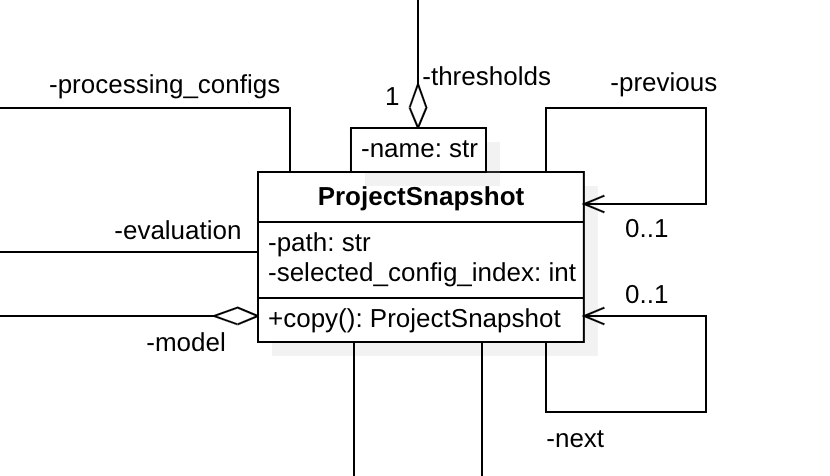
\includegraphics[width=13cm]{entwurf/Entwurf_dokument/img/cls/model/ProjectSnapshot.png}
    \caption{Klassendiagramm von \texttt{ProjectSnapshot}}
\end{figure}

Die Klasse repräsentiert einen Projektzustand zu einem bestimmten Zeitpunkt.
\\\\

\textbf{Attribute}
\begin{itemize}\setlength\itemsep{3em}
\item \texttt{path: str}\\\\
Dateipfad zum Projektverzeichnis, in dem das Projekt (u.~a. automatisch) gespeichert werden soll.
\item \texttt{previous: ProjectSnapshot}\\\\
Projektversion vor der letzten Daten-Operation, die auf dem Projekt durchgeführt wurde.
\item \texttt{next: ProjectSnapshot}\\\\
Projektversion vor der letzten Widerrufs-Operation (\texttt{undo()}), die auf dem Projekt durchgeführt wurde.
\item \texttt{model: Model}\\\\
Diskretes Wahlmodell, welches im Projekt definiert ist.
\item \texttt{processing\char`_configs: list[ProcessingConfig]}\\\\
Liste der im Projekt definierten Verarbeitungskonfigurationen (\texttt{ProcessingConfig}).
\item \texttt{selected\char`_config\char`_index: int}\\\\
Listenindex von \texttt{processing\char`_configs}. Das Listenelement ist die aktuell gewählte Verarbeitungskonfiguration (\texttt{ProcessingConfig}).
\item \texttt{evaluation: Evaluation}\\\\
Auswertung einer Datenverarbeitung, sofern durchgeführt. Ansonsten \texttt{None}.
\item \texttt{thesholds: dict[str, Threshold]}\\\\
Im Projekt konfigurierte Schwellwerte zur Hervorhebung einzelner Auswertungsdaten.
\\\\
\end{itemize}

\textbf{Methoden}
\begin{itemize}\setlength\itemsep{3em}
\item \texttt{copy(): ProjectSnapshot}\\\\
Erstellt eine Kopie des Objekts und gibt diese zurück.
\\\\
\underline{Parameter}\\
\begin{tabular}{lll}
 & Keine Parameter.
\end{tabular}

\underline{Rückgabewert}\\
\begin{tabular}{lll}
 & Kopie des Objekts.\\
\end{tabular}
\end{itemize}

%----------------------------------
\newpage
\subsubsection*{\large{\textbf{ProxyProject}\label{cls:ProxyProject}}}\normalsize
\begin{tabular}{lll}
 Superklassen: & \texttt{Project}\\
 Subklassen: & --
\end{tabular}\\
\begin{figure}[H]%
    \centering
    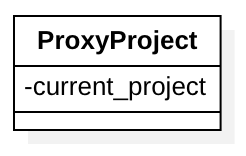
\includegraphics[width=13cm]{entwurf/Entwurf_dokument/img/cls/model/ProxyProject.png}
    \caption{Klassendiagramm von \texttt{ProxyProject}}
\end{figure}

Die Klasse dient entsprechend dem Proxy-Entwurfsmuster zur Erstellung einer zeitunabhängigen Schnittstelle zur Verwaltung eines Projekts. Dies ist notwendig, da die in \texttt{ProjectSnapshot} gehaltenen Daten nicht verändert werden dürfen, da diese als Historie erhalten bleiben sollen. Bei jeder Änderung wird ein neues \texttt{ProjectSnapshot}-Objekt erstellt. Mit dieser Historie werden dann z.~B. die Funktionen \texttt{undo()} und \texttt{redo()} realisiert. Die Proxy-Klasse verweist immer auf den aktuell gültigen \texttt{ProjectSnapshot}.
\\\\

\textbf{Attribute}
\begin{itemize}\setlength\itemsep{3em}
\item \texttt{current\char`_project: ProjectSnapshot}\\\\
Aktuell gültige Version des Projektinhalts.
\\\\
\end{itemize}

\textbf{Methoden}
\begin{itemize}\setlength\itemsep{3em}
\item[] Keine nicht-trivialen Methoden.
\end{itemize}

%----------------------------------
\newpage
\subsubsection*{\large{\textbf{Threshold}\label{cls:Threshold}}}
\textit{\flqq{}immutable\frqq}\normalsize\\\\
\begin{tabular}{lll}
 Superklassen: & --\\
 Subklassen: & --
\end{tabular}\\
\begin{figure}[H]%
    \centering
    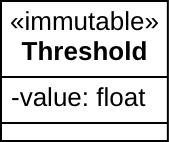
\includegraphics[width=13cm]{entwurf/Entwurf_dokument/img/cls/model/Threshold.png}
    \caption{Klassendiagramm von \texttt{Threshold}}
\end{figure}

Die Klasse repräsentiert einen Darstellungsschwellwert. Hierfür wurde eine eigene Klasse konsturiert, um Erweiterbarkeit zu ermöglichen.
\\\\

\textbf{Attribute}
\begin{itemize}\setlength\itemsep{3em}
\item \texttt{value: float}\\\\
Schwellwert.
\\\\
\end{itemize}

\textbf{Methoden}
\begin{itemize}\setlength\itemsep{3em}
\item[] Keine nicht-trivialen Methoden.
\end{itemize}
%--------------------------------------
\newpage
\subsection{Controller}

Im folgenden Abschnitt werden die Klassen des Paketes \emph{Controller}, so wie sie in Abb.~3.1 dargestellt sind, dokumentiert.

\begin{figure}[H]%
    \centering
    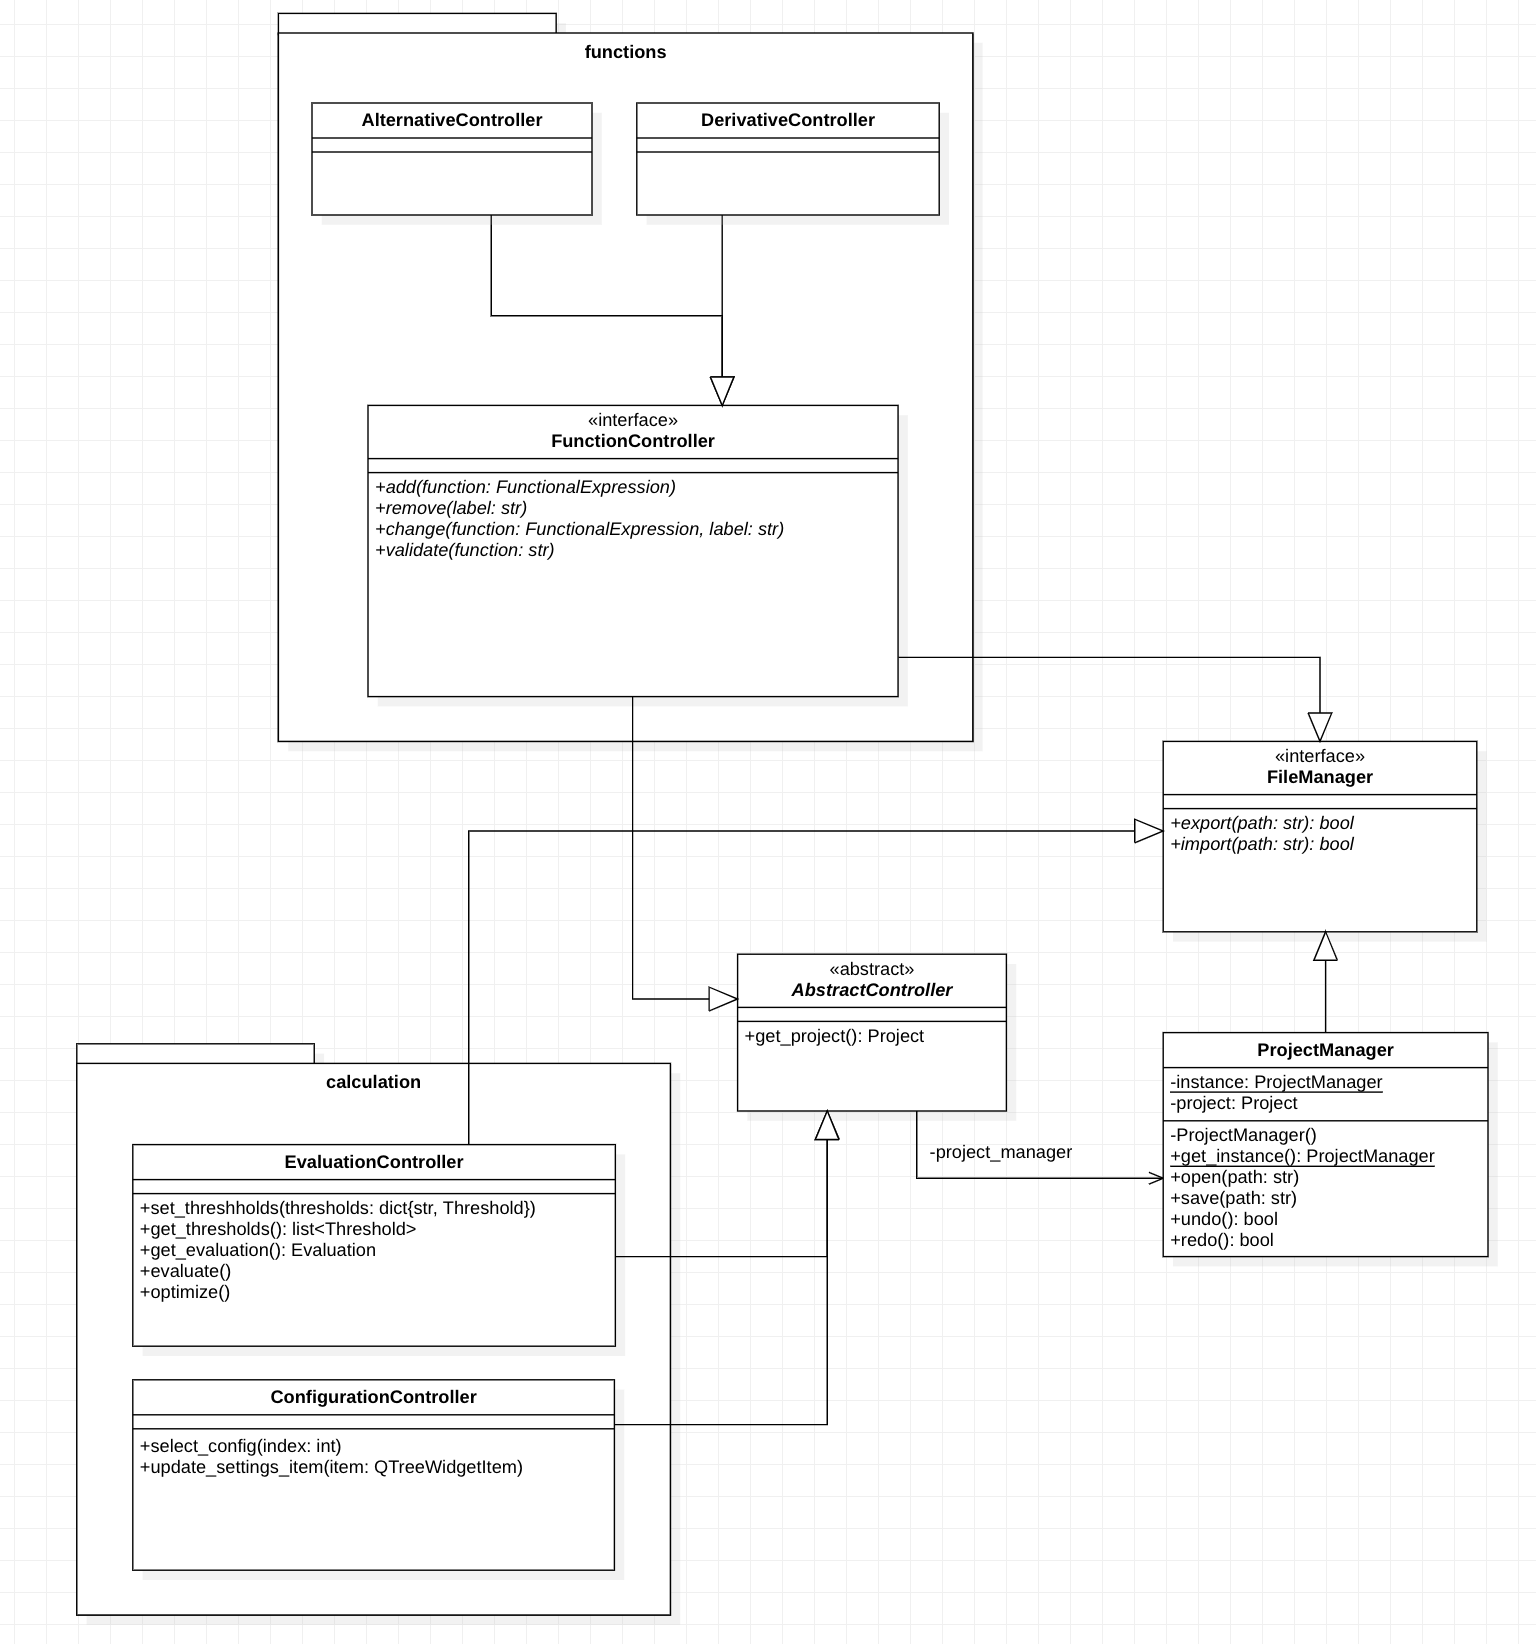
\includegraphics[width=13cm]{entwurf/Floriane/ControllerKlassendiagramm.png}
    \caption{Klassendiagramm Controller}
\end{figure}

Das Package \textit{Controller} beinhaltet sechs Klassen und zwei Interfaces, die den 'Control'-Teil des Modells 'Model-View-Control' umsetzen.

\newpage
\subsubsection*{\large{\textbf{FileManager}\label{cls:FileManager}}}\normalsize
\begin{figure}[H]%
    \centering
    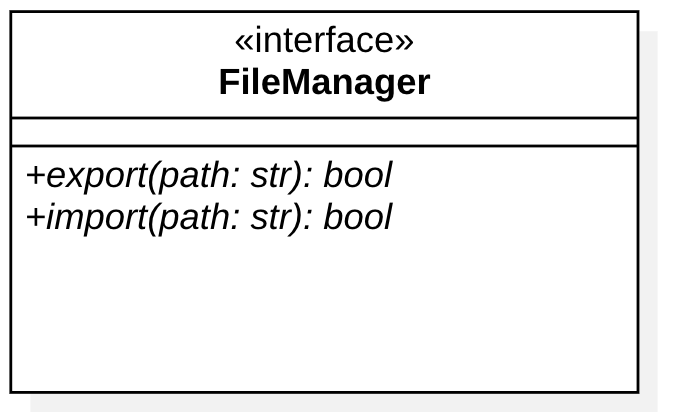
\includegraphics[width=6cm]{entwurf/Floriane/FileManager.png}
    \caption{Interface FileManager}
\end{figure}

Das Interface \textit{FileManager} dient der Interaktion mit externen Dateien. Es wird von allen Klassen im Controller implementiert. Es wurde in einem eigenen Interface entworfen, damit dieses später als Schnittstelle dienen kann, wenn Importe in und Exporte aus anderen Dateiformaten ermöglicht werden sollen.
\newline \newline
\textbf{{Methoden}}
\begin{itemize}
\item \textit{\flqq{}abstract\frqq} \texttt{import(path:str):bool} \newline Dient dem Import aller notwendigen Dateien und behandelt den Zugriff auf diese. Die Controller implementieren die Methode um sie für die jeweiligen Daten bzw. Funktionen zu nutzen.
\\\\
\underline{{Parameter}}

\begin{tabular}{lll}
 & \texttt{path:str} & Der Pfad zum Speicherort der zu importierenden Datei. \\
\end{tabular}

\underline{{Rückgabewert}}

\begin{tabular}{lll}
 & \texttt{bool} & Ob der Import erfolgreich war. \\
\end{tabular}

\item \textit{\flqq{}abstract\frqq}\texttt{export(path:str):bool} \newline Führt den Export einer Datei zu einem bestimmten Pfad aus. Diese Methode wird vom jeweiligen Controller implementiert.
\\\\
\underline{{Parameter}}

\begin{tabular}{lll}
 & \texttt{path:str} & Der Pfad zum Speicherort der zu speichernden Datei. \\
\end{tabular}

\underline{{Rückgabewert}}

\begin{tabular}{lll}
 & \texttt{bool} & Ob der Export erfolgreich war. \\
\end{tabular}
\end{itemize}



\newpage
\subsubsection*{\large{\textbf{ProjectManager}\label{cls:ProjectManager}}}\normalsize

\begin{figure}[H]%
    \centering
    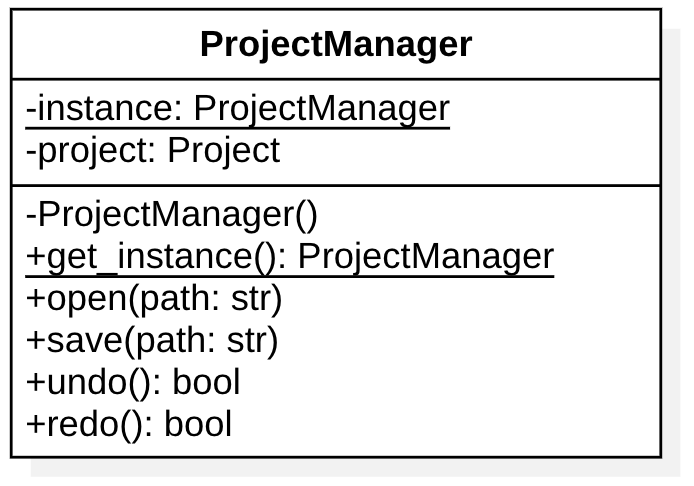
\includegraphics[width=7cm]{entwurf/Floriane/ProjectManager.png}
    \caption{Klasse ProjectManager}
\end{figure}

Der ProjectManager dient der Kontrolle der Project Objekte. Er wurde nach dem Muster des Singletons entworfen, indem er einen privaten Konstruktor hat, eine statische Instanz und eine statische Methode, die diese Instanz zurück gibt. So wird verhindert, dass es mehrere ProjektManager gibt, die möglicherweise auf verschiedene Projekte verweisen. Die anderen Controller erhalten Zugriff auf ihn durch die abstrakte Klasse AbstractController, die den ProjektManager als privates Attribut besitzt.
\newline\newline
\textbf{\large{Implementiert}} FileManager 
\newline\newline
\textbf{\large{Attribute}}
\begin{itemize}
\item \flqq{}static\frqq \texttt{instance: ProjectManager}\\ Die einzige Instanz dieser Klasse.
\item \texttt{project:Project}\\Private instanz der Klasse ProxyProject zur Projektverwaltung. Diese wird für alle Funktionen die das Projekt verändern und neue Snapshot. 
\end{itemize}\leavevmode\newline
\textbf{\large{Methoden}}
\begin{itemize}
\item \texttt{ProjectManager()}\\ Privater Konstruktor der Klasse zum Sicherstellen, dass es die Klasse nur eine Instanz besitzt.

\item \flqq{}static\frqq \texttt{get\_instance(): ProjectManager}\\ Zugriff auf den Projektmanager.\\\\
\underline{{Rückgabetypen}}\\
\begin{tabular}{llp{8.5cm}}
 & \texttt{ProjectManager} & Die einzige instanz des ProjektManagers. \\
\end{tabular}
\item \texttt{open(path:str)}\\ Öffnet ein neues oder bestehendes Projekt.\\\\
\underline{{Parameter}}\\
\begin{tabular}{llp{8.5cm}}
 & \texttt{path:str} & Der Pfand an dem das Projekt bereits besteht, oder das neue Projekt gespeichert werden soll. \\
\end{tabular}

\item \texttt{save(path:str)}\\ Speichern des Projektes.\\\\
\underline{{Parameter}}\\
\begin{tabular}{lll}
 & \texttt{path:str} & Der Pfad an dem das Projekt gespeichert werden soll. \\
\end{tabular}
\item \texttt{undo(): bool}\\ Rückgängigmachen der letzten Änderung. Im Projekt wird der aktuelle ProjectSnaphot durch den vorherigen ersetzt.\\\\
\underline{{Rückgabetypen}}\\
\begin{tabular}{lp{10.7cm}}
 & \texttt{bool}  True falls Änderung des Projektsnapshots erfolgreich war.\\
\end{tabular}
\item \texttt{redo(): bool): ProjectManager}\\ Wiederherstellen des zuletzt rückgängig gemachten Schrittes. Im Projekt wird der aktuelle Snapshot durch den folgenden ersetzt falls dieser existiert.\\\\
\underline{{Rückgabetypen}}\\
\begin{tabular}{lp{10.7cm}}
 & \texttt{bool}  True falls Änderung des Projektsnapshots erfolgreich war.\\
\end{tabular}
\end{itemize}


\newpage
\subsubsection*{\large{\textbf{AbstractController}\label{cls:AbstractController}}}\normalsize
\begin{figure}[H]%
    \centering
    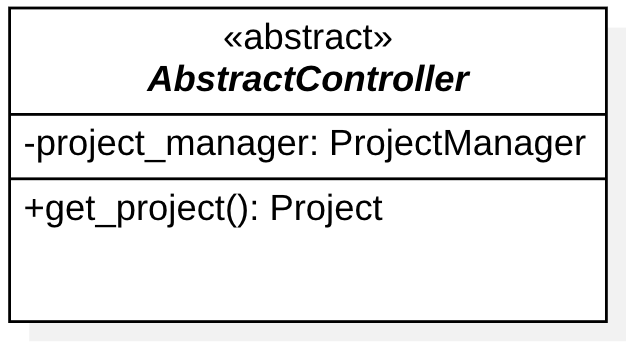
\includegraphics[width=6cm]{entwurf/Floriane/AbstractController.png}
    \caption{Abstrakte Klasse AbstractController}
\end{figure}


Abstrakte Klasse die als Verbindung zum ProjektManager dient. Die anderen Controller, die nicht für Speicherung oder Projektauswahl zuständig sind, können durch die geerbte Methode \texttt{get\_project()} auf das Projekt zugreifen. Da die Controller nicht das Attribut \texttt{project\_manager} erben, können sie den Projektmanager aber nicht ändern oder dessen Funktionen verwenden. Er dient in der Rolle Kollege zum 
Projektmanager im 'Vermittler' Entwurfsmuster.
\\\\
\textbf{\large{Attribute}}
\begin{itemize}
\item \texttt{project\_manager:ProjectManager}\\ Der Projektmanager des Programms. Dieser kann nicht neu gesetzt werden. Er ist privat, damit er nicht vererbt wird und die Kindklassen keinen direkten Zugriff besitzen.
\end{itemize}\leavevmode\newline
\textbf{\large{Methoden}}
\begin{itemize}
\item \texttt{get\_project():Project}\\ Methode als Schnittstelle zwischen Projekt und den Controllern.\\\\
\underline{{Rückgabewert}}\\
\begin{tabular}{lll}
 & \texttt{Project} & Das aktuelle Projekt. \\
\end{tabular}
\end{itemize}



\newpage
\subsubsection*{\large{\textbf{FunctionController}\label{cls:FunctionController}}}\normalsize

\begin{figure}[H]%
    \centering
    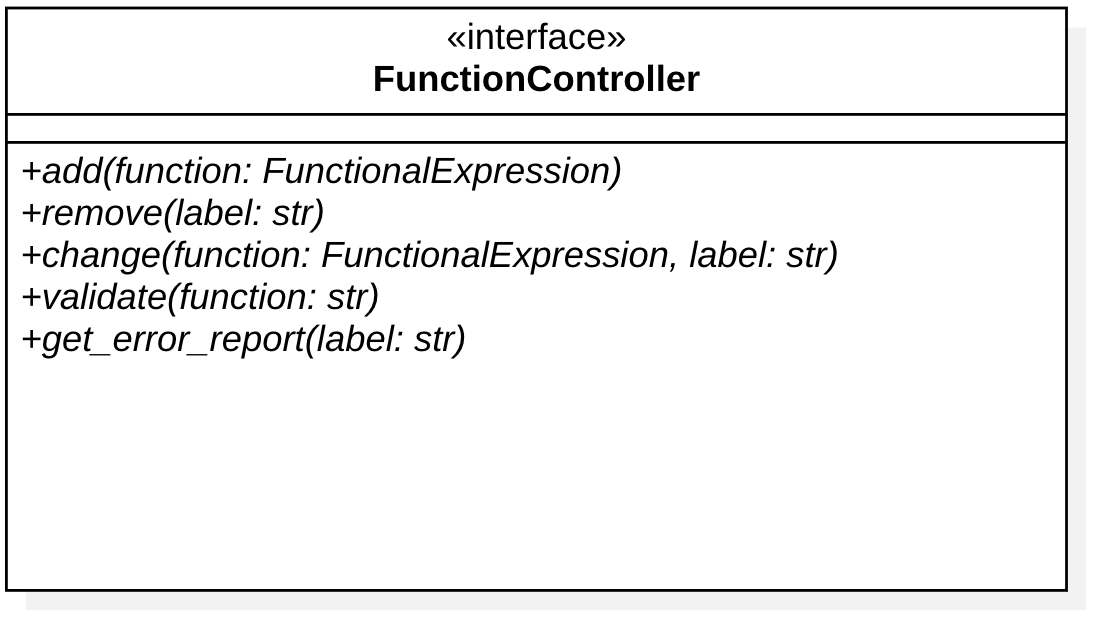
\includegraphics[width=10cm]{entwurf/Floriane/FunctionController.png}
    \caption{Abstrakte Klasse FunctionController}
\end{figure}


Controller Schablone zur Verwaltung der Funktionen. Das Interface besitzt die Funktionen die notwendigerweise von den konkreten Controllern zur Funktionsverwaltung implementiert werden müssen.
\newline\newline
\textbf{\large{Implementiert}} FileManager, AbstractController
\newline\newline
\textbf{\large{Methoden}}
\begin{itemize}
\item \flqq{}abstract\frqq \texttt{add(label:str, function:FunctionalExpression)}\\ Hinzufügen neuer Funktionen zum aktuellen Projekt.\\\\
\underline{{Parameter}}\\
\begin{tabular}{lp{10.7cm}}
 & \texttt{function:FunctionalExpression}  Instanz der Klasse FunctionalExpression, die die Funktion die hinzugefügt werden soll enthält. \\
  & \texttt{label:str} Vom Nutzer gegebener Name der Funktion. \\
\end{tabular}
\item \flqq{}abstract\frqq \texttt{remove(label:str)}\\ Entfernung einer Funktion aus dem aktuellen Projekt. \\\\
\underline{{Parameter}}\\
\begin{tabular}{lll}
 & \texttt{label:str} & Name der Funktion zur Identifizierung im Model. \\
\end{tabular}
\item \flqq{}abstract\frqq \texttt{change(function:FunctionalExpression, label:str)}\\ Änderung einer Funktion im Projekt.\\\\
\underline{{Parameter}}\\
\begin{tabular}{lp{10.7cm}}
 & \texttt{function:FunctionalExpression}:  Neuer funktionaler Ausdruck als Instanz der Klasse FunctionalExpression.\\
 & \texttt{label:str}:  Name der Funkton zur Identifizierung im Model. \\
\end{tabular}
\item \flqq{}abstract\frqq \texttt{validate(function:str): FunctionalExpression}\\ Validierung der Nutzereingabe. Hier wird überprüft ob der Builder es der Klasse FunctionalExpression erlauben soll die Nutzereingabe als Python Code zu interpretieren. Code, der über einen mathematischen Ausdruck hinausgeht wird in dieser Methode abgefangen, bevor er evaluiert würde. Falls die Validierung erfolgreich ist, wird eine FunktionalExpression zurückgegeben. Falls nicht wird None zurückgegeben und die Nutzereingabe verworfen. Hier wird ausdrücklich nicht die Korrektheit des Funktionsausdrucks überprüft, sondern nur seine Existenz.\\\\
\underline{{Parameter}}\\
\begin{tabular}{lp{10.7cm}}
 & \texttt{function:str}  Nutzereingabe, die einen mathematischen Ausdruck wiederspiegeln soll. \\
\end{tabular}
\newline\newline
\underline{{Rückgabewert}}\\
\begin{tabular}{lp{10.7cm}}
 & \texttt{FunctionalExpression} Funktion als Objekt der Klasse FunctionalExpression so wie sie im Programm verarbeitet wird. \\
\end{tabular}


\item \flqq{}abstract\frqq \texttt{get\_error\_report(label:str)}\\ Ausführung der Evaluierung einer Funktion vom Controller aus. Dabei wird der zugrundeliegende mathematische Ausdruck evaluiert, sowie mögliche Fehler gefunden. Diese werden werden den Funktionenzugeordnet, sodass der View sie anzeigen kann. \\\\
\underline{{Parameter}}\\
\begin{tabular}{lp{10.7cm}}
 & \texttt{label:str} Name der Funktion, der dem Nutzer angezeigt wird. \\
\end{tabular}
\end{itemize}


\newpage
\subsubsection*{\large{\textbf{AlternativeController}\label{cls:AlternativeController}}}\normalsize

\begin{figure}[H]%
    \centering
    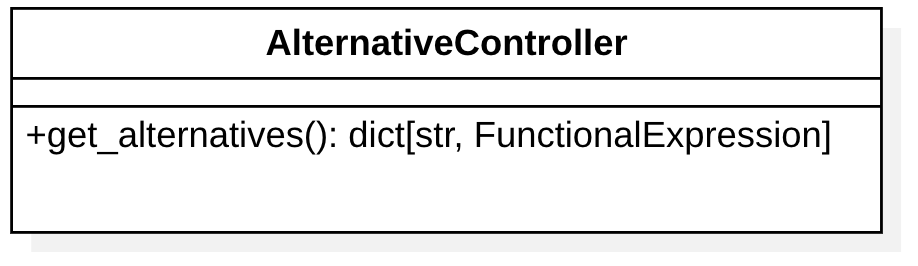
\includegraphics[width=10cm]{entwurf/Floriane/AlternativeController.png}
    \caption{AlternativeController}
\end{figure}

Die Klasse \textit{AlternativeController} ist zuständig für die Verwaltung der Alternativen. Sie implementiert das Interface \textit{FunctionController} mit den Funktionen add, change, remove und validate im Bezug auf die Alternativen.
\newline\newline
\textbf{\large{Implementiert}} FunctionController \\\\
\textbf{\large{Methoden}}
\begin{itemize}
\item \texttt{get\_alternatives(): dict[str, FunctionalExpression]}\\ Zugriff auf die im Projekt vorhandenen Alternativen.\\\\
\underline{{Rückgabetypen}}\\
\begin{tabular}{lp{10.7cm}}
 & \texttt{dict[str, FunctionalExpression]}  Dictionary mit allen Alternativen. Dabei sind die Namen der Alternativen die Schlüssel und die Funktionen in Form von FunctionalExpression Instanzen die Werte.\\
\end{tabular}
\end{itemize}


\newpage
\subsubsection*{\large{\textbf{DerivativeController}\label{cls:DerivativeController}}}\normalsize

\begin{figure}[H]%
    \centering
    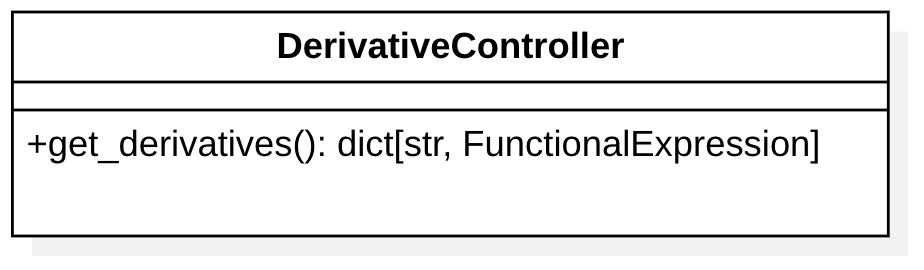
\includegraphics[width=10cm]{entwurf/Floriane/DerivativeController.png}
    \caption{DerivativeController}
\end{figure}

Die Klasse \textit{DerivativeController} ist zuständig für die Verwaltung der Attributsableitungsfunktionen. Sie implementiert das Interface \textit{FunctionController} mit den Funktionen add, change, remove und validate im Bezug auf die Attributsableitungsfunktionen.\\\\
\textbf{\large{Implementiert}} FunctionController 
\textbf{\large{Methoden}}
\begin{itemize}
\item \texttt{get\_derivatives(): dict[str, FunctionalExpression]}\\ Zugriff auf die im Projekt vorhandenen Attributsableitungen.\\\\
\underline{{Rückgabetypen}}\\
\begin{tabular}{lp{10.7cm}}
 & \texttt{dict[str, FunctionalExpression]}  Dictionary mit allen Attributsableitungsfunktionen. Dabei sind die Namen der Attribute die Schlüssel und die Funktionen in Form von FunctionalExpression Instanzen die Werte im Dictionary.\\
\end{tabular}
\end{itemize}

\newpage
\subsubsection*{\large{\textbf{ConfigurationController}\label{cls:ConfigurationController}}}\normalsize

\begin{figure}[H]%
    \centering
    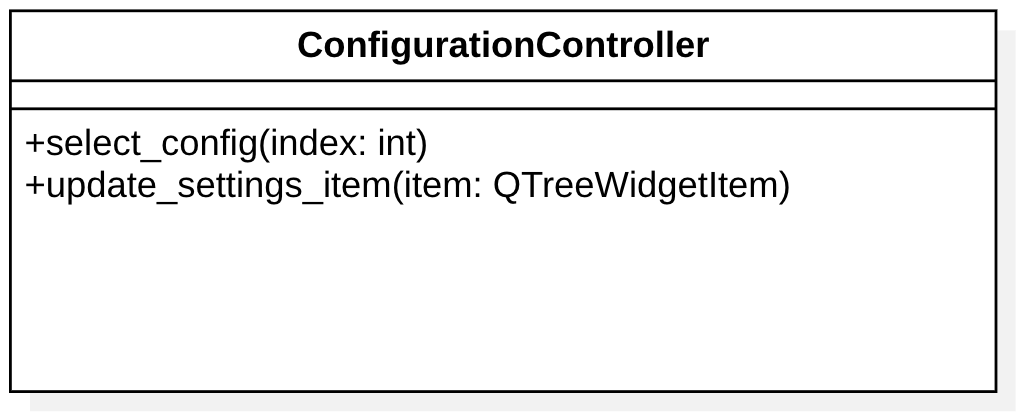
\includegraphics[width=10cm]{entwurf/Floriane/ConfigurationController.png}
    \caption{ConfigurationController}
\end{figure}

Verwaltet die Konfigurationen zur Modellberechnung. Es können die bereits implementierten Modell Konfigurationen aus einer Liste ausgewählt werden. \\\\
\textbf{\large{Methoden}}
\begin{itemize}
\item \texttt{select\_config(index:int)}\\ Methode zur Auswahl anderer Konfigurationen aus der Liste der bestehenden Konfigurationen.\\\\
\underline{{Parameter}}\\
\begin{tabular}{lp{10.7cm}}
 & \texttt{index:int} Index der ausgewählten Konfiguration in der Konfigurationsliste. \\
\end{tabular}
\item \texttt{update\_settings\_item(item: QTreeWidgetitem))}\\ Aktualisiert die Einstellungen im System entsprechend der Nutzereingaben im Frontend. Diese werden aus dem übergebenen Widget ausgelesen und in die ProcessingConfig übertragen.\\\\
\underline{{Parameter}}\\
\begin{tabular}{lp{10.7cm}}
 & \texttt{item:QTreeWidgetitem} Das Widget aus dem Frontend, das die Nutzereingaben enthält. \\
\end{tabular}
\end{itemize}


\newpage
\subsubsection*{\large{\textbf{EvaluationController}\label{cls:EvaluationController}}}\normalsize

\begin{figure}[H]%
    \centering
    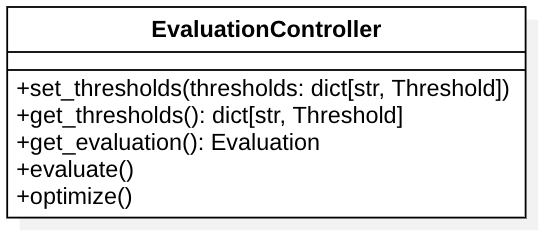
\includegraphics[width=10cm]{entwurf/Floriane/EvaluationController.png}
    \caption{EvaluationController}
\end{figure}

Kontrolle der Berechnungen des Programms. Ist zuständig für die Verwaltung der Schwellwerte, Modelloptimierungen und Evaluierungen.\\\\
\textbf{\large{Methoden}}
\begin{itemize}
\item \texttt{set\_thresholds(thresholds: dict{str, Threshold})}\\ Änderung der Schwellwerte, die im Programm hinterlegt sind.\\\\
\underline{{Parameter}}\\
\begin{tabular}{lp{10.7cm}}
 & \texttt{thresholds:dict[str,Threshold]} Dictionary, das die Namen der Schwellwarte als Schlüssel und die Schwellwertobjekte als Werte enthält. \\
\end{tabular}
\item \texttt{get\_thresholds(): dict[str, Threshold]}\\ Zugriffsmethode auf die Liste der Schwellwerte, die im Programmhinterlegt sind.\\\\
\underline{{Rückgabewerte}}\\
\begin{tabular}{lll}
 & \texttt{dict[str, Threshold]} & Liste aus Schwellwertobjekten. \\
\end{tabular}
\item \texttt{evaluate()}\\ Aufruf der Modellevaluierung im aktuellen Projekt.
\item \texttt{get\_evaluation():Evaluation}\\ Zugriff auf die bereits berechnete Modellevaluierung im aktuellen Projekt.\\\\
\underline{{Rückgabewerte}}\\
\begin{tabular}{lll}
 & \texttt{Evaluation} & Modellevaluierung, wie sie im Projekt berechnet wurde \\
\end{tabular}
\item \texttt{optimize()}\\ Methode zum Aufruf der Modelloptimierung im Projekt.\\
\end{itemize}





\newpage
\section{Softwareablauf}
\subsection{Projektmanagement}
\begin{figure}[H]%
    \centering
    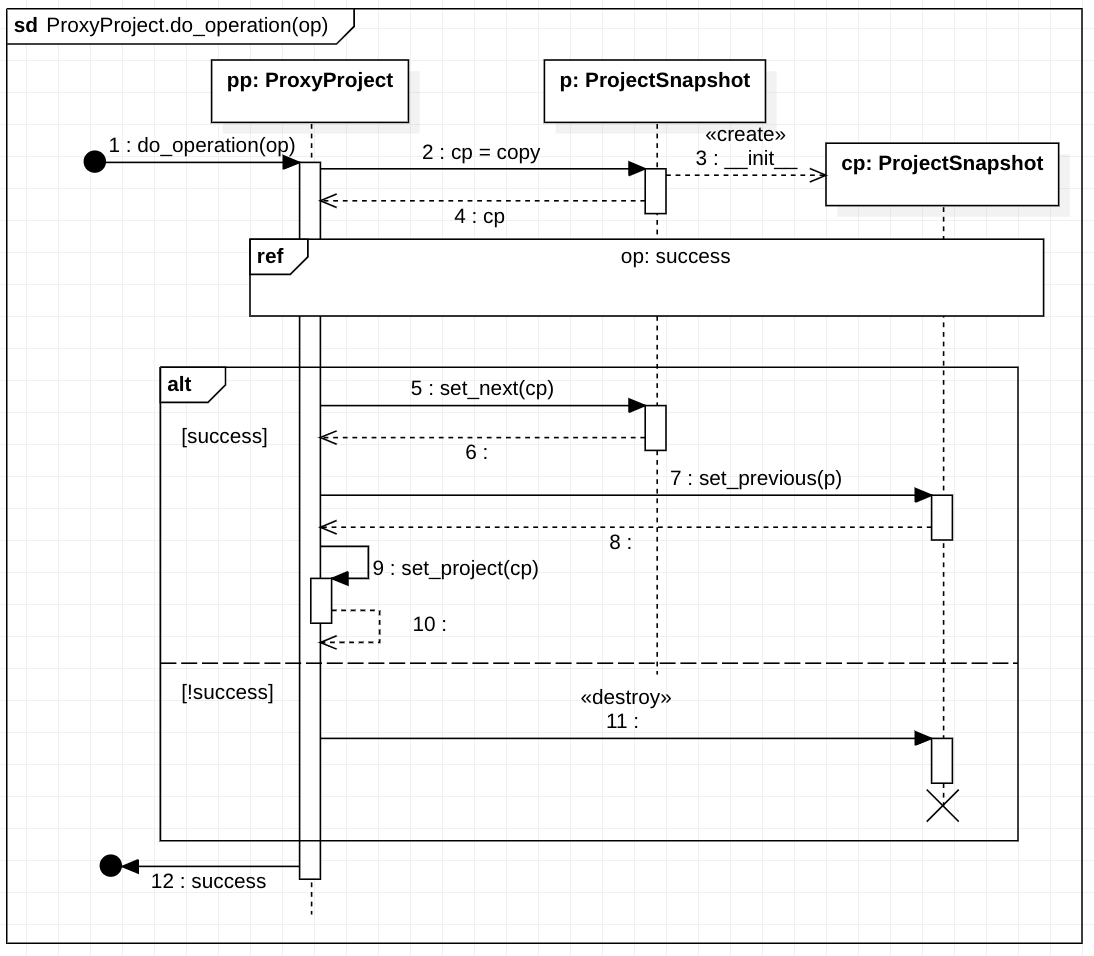
\includegraphics[width=13cm]{entwurf/Entwurf_dokument/img/Michael/sd_ProxyProject.do_operation.png}
    \caption{Sequenzdiagramm der Anwendung einer Projektoperation}
    \label{fig:sq:do_operation}
\end{figure}

Die Veränderung der Projektdaten ist Bestandteil jedes Anwendungsfalls. Aus diesem Grund bietet es sich an, für die Anwendung einer Projektoperation ein einheitliches Vorgehen zu entwerfen. Dieses ist in Abbildung \ref{fig:sq:do_operation} dargestellt.\\

\begin{enumerate}
    \item[1.] Befehl \texttt{do\char`_operation(op)} erreicht \texttt{pp:ProxyProject}
    \item[2.] Kopie des Projektzustands wird angestoßen
    \item[3.] Kopie des Projektzustands wird angelegt (\texttt{cp:ProjectSnapshot})
    \item[4.] Kopie wird an \texttt{ProxyProject} zurückgegeben
    \item[4.5.] Operation \emph{op} wird auf den neu angelegten Projektzustand (\emph{cp}) angewendet
    \item[] Wenn die Operation erfolgreich verlaufen ist:
    \begin{enumerate}
        \item[5.] Die neu angelegte Kopie (\emph{cp}) wird als Nachfolgezustand im alten Projektzustand (\emph{p}) hinterlegt.
        \item[7.] Im neuen Projektzustand (\emph{cp}) wird ebenso der alte Projektzustand als Vorgängerzustand (\emph{p}) hinterlegt.
        \item[9.] Wenn die Operation erfolgreich verlaufen ist, wird abschließend noch im \texttt{ProxyProject} (\emph{pp}) der neue Projektzustand (\emph{cp}) als aktueller Zustand hinterlegt.
    \end{enumerate}
    \item[] Wenn die Operation fehlgeschlagen ist:
    \begin{enumerate}
        \item[11.] Kopie des Projektzustands wird gelöscht.
    \end{enumerate}
    \item[12.] Zurückgeben, ob Operation erfolgreich.
    
\end{enumerate}

\textbf{\large{Neues Projekt öffnen}}
\begin{figure}[H]%
    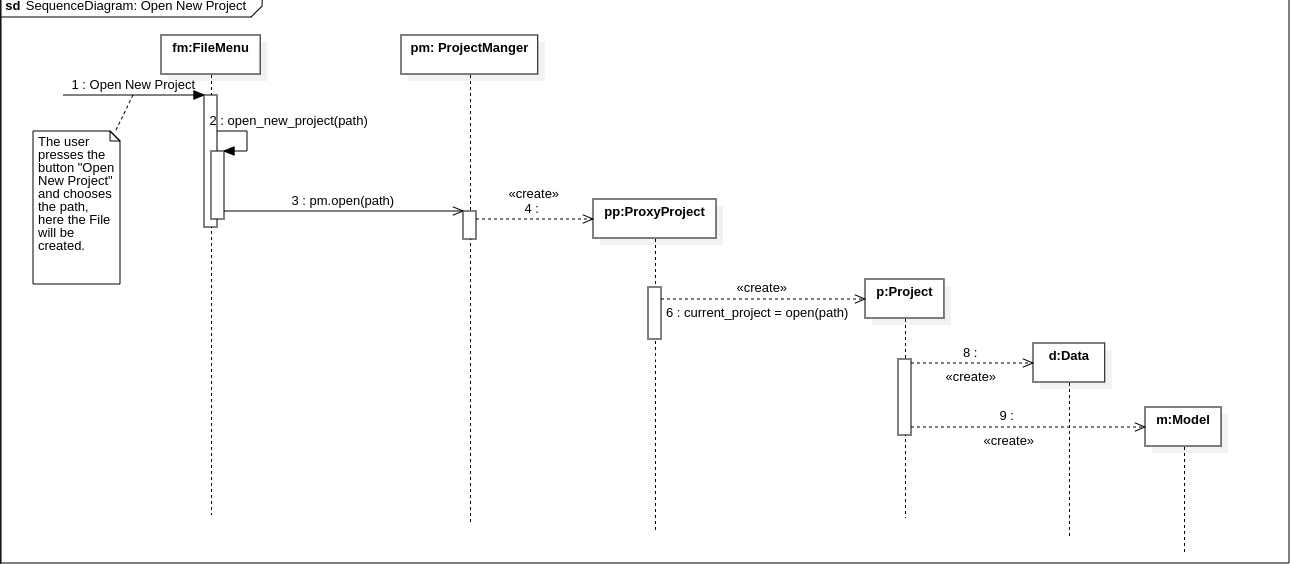
\includegraphics[width=15cm]{entwurf/Entwurf_dokument/img/Alissa/SQOpenNewProject3.png}
    \caption{SequenzDiagramm für Neues Projekt öffnen}
    \label{fig:sq:openNewProject}
\end{figure}
Wenn ein Nutzer ein Projekt erstellen möchte, dann muss er zuerst ein neues Projekt erstellen lassen und dann die Erhebungsdaten importieren. Im folgenden wird die Sequenzediagramm \ref{fig:sq:openNewProject} erläutert:

\begin{enumerate}
    \item[1.] Der Nutzer klickt auf die Schaltfläche "Open New Project\" im \textit{File Menu}.
    \item[1.5] Der Nutzer wählt über dem Datei-Dialog den Speicherort.  
    \item[2.] Die Funktion \texttt{open\char`_new\char`_project} in der Klasse \textit{FileMenu} aufgerufen. Als Parameter \textit{path} wird der gewählte Speicherort als String übergeben.
    \item[3.] In der Funktion \textit{open\char`_new\char`_project} wird der Controller(\textit{ProjectManager}) durch \textit{open(path)} aufgerufen.
    \item[4.] Durch den Controller wird ein \textit{ProxyProject} Objekt erstellt.
    \item[5.] Der \textit{ProxyProject} Objekt erstellt automatisch (Mit aufrufen seiner Konstruktor) einen Objekt vom Typ \textit{Project}
    \item[6.] Der \textit{Project}\textendash Objekt erstellt widerrum Zwei Objekte. Einmal vom Typ \textit{Data} und dieser wird bei Erstellung des Objekts vom Typ \textit{Model} benötigt. 
\end{enumerate}

Somit wird ein neues Projekt geöffnet.
\begin{figure}[H]%
    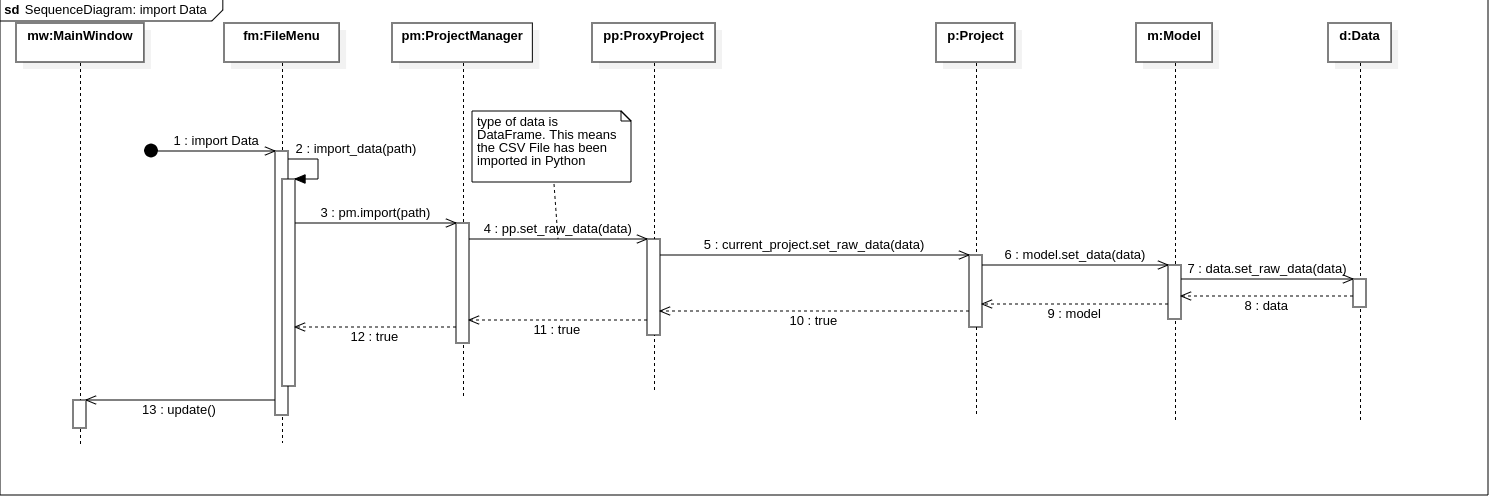
\includegraphics[width=15cm]{entwurf/Entwurf_dokument/img/Alissa/SQImportDataFinal.png}
    \caption{SequenzDiagramm für Daten Importieren}
    \label{fig:sq:importData}
\end{figure}
Nun soll der Nutzer die Erhebungsdaten importieren wie in der Abbildung \ref{fig:sq:importData} beschrieben. Im folgenden wir der Ablauf erläutert:
\begin{enumerate}
    \item[1.] Der Nutzer klickt auf der Schaltfläche "Import Data" im \textit{File Menu} und wählt durch die Datei Dialog die zu importierenden CSV Datei. Dadurch wird die Funktion \texttt{import\char`_data(path)} im \textit{FileMenu} aufgerufen.
    \item[2.] Dieser ruft den \textit{ProjectManager}, in dem die Methode \textit{import\char`_data} aufgerufen wird.
    \item[3.] In der Methode \textit{import\char`_data} wird die CSV Datei geöffnet. Nun stehen die Daten als \textit{data} vom typ \textit{DataFrame}
    \item[4.] Die Daten werden an dem \textit{ProxyProject} übergeben, dieser ordnet dem \textit{Project}\textendash die Daten \textit{data} zu.
    \item[5.] Der \textit{Project}\textendash Objekt leitet die Daten an dem \textit{Model} weiter, und diese werden dann an dem \textit{Data} weitergeleitet. Dadurch wird es möglich, die Daten zu verwalten.
    \item[6.] Als letzter Schritt muss noch die \textit{FileMenu} die \textit{MainWindow} informieren, damit dieser die importierte Daten anzeigt. 
\end{enumerate}
\newpage
\textbf{\large{Projekt Öffnen}}
\begin{figure}[H]%
    \centering
    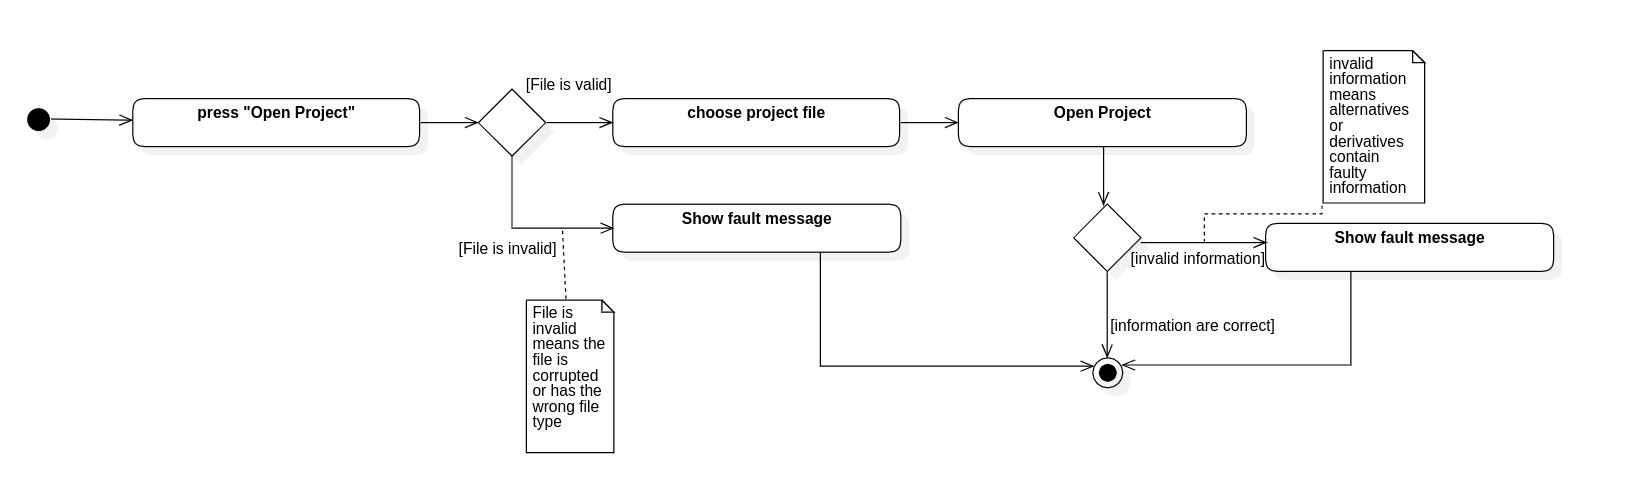
\includegraphics[width=13cm]{entwurf/Entwurf_dokument/img/Alissa/OpenProjectAD.png}
    \caption{Aktivitätsdiagramm Projekt öffnen}
\end{figure}
Der Nutzer kann auch ein Projekt öffnen, den er vorher erstellt hat. Dafür macht er folgendes:
\begin{enumerate}
    \item[1.] er klickt auf "Open Project". Diese befindet sich in der Datei Menü (FileMenu).
    \item[2.] Sollte die Datei valide sein. Das heißt es die Datei ist nicht korrupt und entspricht den erwarteten Dateityp, dann wird das Projekt geöffnet.
    \item[3.] Ansonsten erscheint eine Fehler Meldung und der Vorgang wird abgeborechen.
    \item[4.] Nach dem der Projekt geöffnet wurde, wird der Nutzer über Fehlerhafte Daten (Alternativen oder Ableitungen) informiert, falls es welche gibt. 
\end{enumerate}

\textbf{\large{Projekt Speichern}}
\begin{figure}[H]%
    \centering
    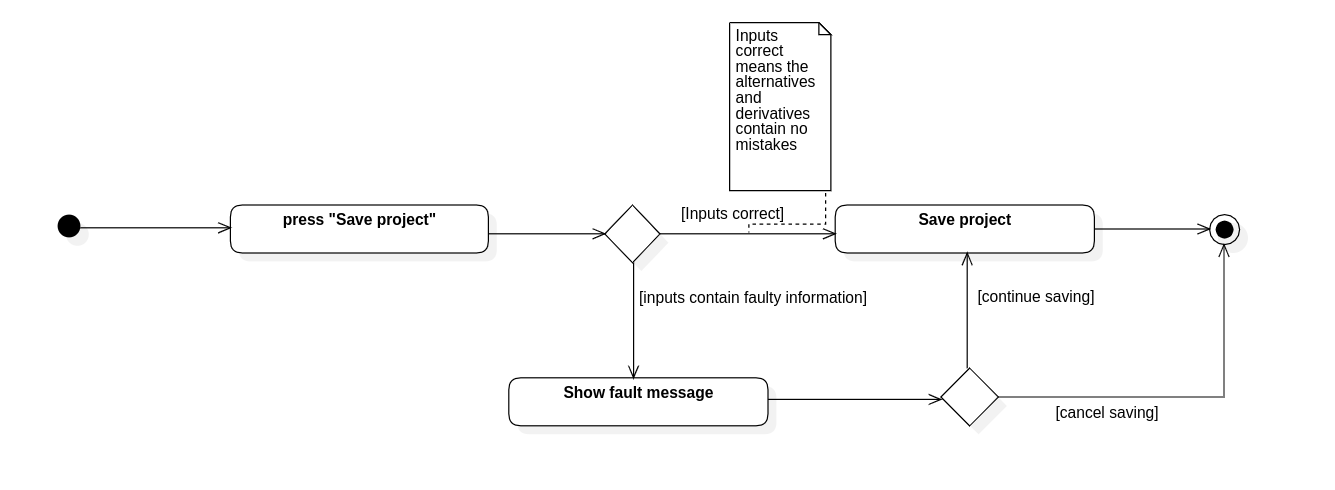
\includegraphics[width=13cm]{entwurf/Entwurf_dokument/img/Alissa/SaveProjectAD.png}
    \caption{Aktivitätsdiagramm für Projekt speichern}
\end{figure}
Damit der Nutzer den Projekt speichert, macht er folgendes:
\begin{enumerate}
    \item[1.] Der Nutzer klickt auf \"Save Project\", welche in der Datei\textendash Menü (File\textendash zu finden) ist.
    \item[2.] Wenn alle Nutzer Eingaben (Ableitungen und Alternativen) Korrekt sind, dann wird das Projekt gespeichrt.
    \item[3.] Ansonsten wird der Nutzer über die Existenz von fehlerhaften Eingaben informiert.
    \item[3.] Der Nutzer kann den Projekt trotz die Fehler speichern oder er bricht den vorgang ab.
\end{enumerate}
Alternativ kann der Nutzer auch einen anderen Speicherort wählen, anstatt die aktuelle Speicherort des projekts.

\begin{figure}[H]%
    \centering
    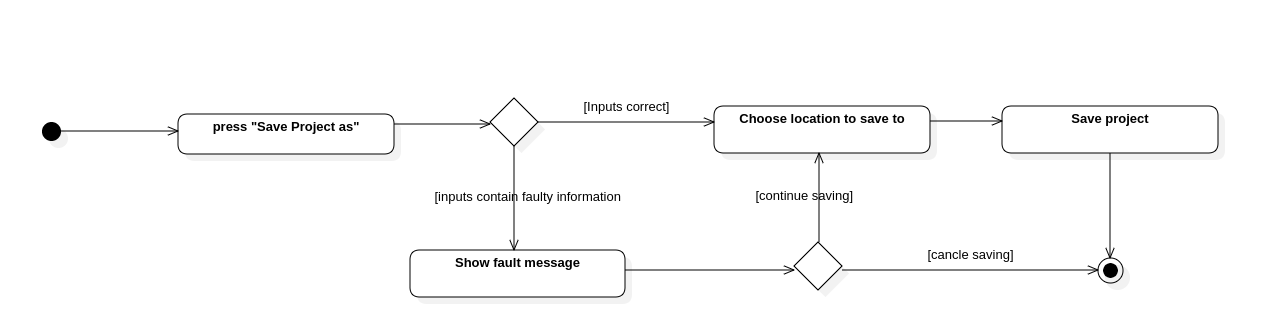
\includegraphics[width=13cm]{entwurf/Entwurf_dokument/img/Alissa/SaveProjectAsAD.png}
    \caption{Aktivitätsdiagramm für Projekt Speichern als}
\end{figure}
Dafür kann der Nutzer die Option \textit{Save Project As} im Datei\textendash Menü wählen. Der Abluf ist mit dem Option \textit{Save project} sehr ähnlich, nur hier kann der Nutzer einen Speicherort mit dem Datei\textendash Dialog wählen.
\\\\
\textbf{\large{CSV Datei exportieren}}
\begin{figure}[H]%
    \centering
    \includegraphics[width=13cm]{entwurf/Entwurf_dokument/img/Alissa/ExportCSVAD.png}
    \caption{Aktivitätsdiagramm für CSV Datei exportieren}
    \label{ad:adExportData}
\end{figure}
Dieser Aktivitätsdiagram \ref{ad:adExportData} beschreibt den Ablauf, wenn der Nutzer die Erhebungsdaten mit den ABleitungen exportieren möchte.
\begin{enumerate}
    \item[1.] Der Nutzer klickt auf \textit{Export Data} in der Datei\textendash Menü
    \item[2.] Wenn es Ableitungen gibt, die fehlerhaft sind, dann wir dem Nutzer eine Fehlermeldung gezeigt. Der Nutzer hat dann die Wahl, den Exportier Vorgang fortzuführen oder abzubrechen.
    \item[3.] Der Nutzer wählt den Speicherort, wo die Daten exportiert werden müssen.
\end{enumerate}

\newpage
\subsection{Attributsmanagement}


Das Attributsmanagement besteht aus fünf verschiedene Funktionen: Ändern, Hinzufügen, Löschen, Importieren und Exportieren von Attributsableitungen. Die Attributsableitungen sind im Programm Instanzen der Klasse \textit{FunctionalExpression}, die in einem \textit{Dictionary} in der Klasse \textit{Data} des jeweiligen \textit{ProjectSnapshot} hinterlegt sind. Referenziert werden sie über einen vom Nutzer zugewiesenem Namen.

\subsubsection{Änderung einer Attributsableitung}
Die Abläufe dieser Funktionen werden nun beispielhaft anhand eines Sequenzdiagramms (vgl. Abb.~\ref{fig:sq:ChangeDerivativeSequenceDiagram}) beschreiben. Dieses behandelt die Aktione des Nutzers eine bestehende Attributsableitung zu ändern. Vorraussetzung dafür ist, dass mindestens eine Attributsableitung vorhanden ist. Die Sequenzen des Hinzufügens und des Importes funktionieren analog und werden nicht einzeln behandelt.

\begin{figure}[H]%
    \centering
    \includegraphics[width=12cm]{entwurf/Floriane/ChangeDerivative.png}
    \caption{Änderung einer Attributsableitung Sequenzdiagramm}
    \label{fig:sq:ChangeDerivativeSequenceDiagram}
\end{figure}

Zuerst wählt der Nutzer eine dargestellte Attributsableitung aus, und ändert den darin vorhandenen mathematischen Ausdruck (vgl. Schritt 1). \\\\Das \textit{ColumnWidget} nimmt diese Änderung wahr und ruft im zugewiesenen \textit{DerivativeController} die Funktion \texttt{change(label, expression)} auf (vgl. Schritt 2). Dabei ist \texttt{label} ein \textit{String} der den Namen dieser Attributsableitung festlegt und \texttt{expression} die vorgesehene mathematische Formel. Im dritten Schritt wird die \texttt{expression} validiert und auf Sicherhit überprüft (vgl Schritt 3, vgl Abb XY2). Genaueres dazu in -----. \\\\
War die Validierung erfolgreich wird eine Instanz der Klasse \textit{FunctionalExpression} erstellt, die diesen Ausdruck wiedergibt (Schritt 4). Nun ruft der \textit{DerivativeController} über den \textit{Projektmanager} das \textit{ProxyProject} auf (Schritt 5, 6).\\\\
Das \textit{ProxyProject} führt die Funktion \texttt{set\_derivatives(label, new\_derivative)} aus (Schritt 7). Das Funktionsobject \texttt{new\_derivative} wird dabei dem ProxyProjekt übergeben, das alle Funktionen die auf dem Projekt ausgeführt werden dürfen übernimmt und dabei bei jeder Änderung einen neuen Snapshot erstellt (vgl ----, Schritt 8).\\\\
In dem neuen ProjektSnapshot werden dann die Änderungen durchgeführt (Schritt 9), indem erst auf die bestehende Data-Instanz zugegriffen wird (Schritt 10, 11) und anstelle einer Änderung eine neue Data-Instanz erzeugt wird (Schritt 12, 13), die die geänderte Ableitungsfunktion, sowie alle anderen Daten der vorherigen Data-Instanz enthält. Zu beachten ist, dass die Ableitungsfunktionen nicht geändert werden, sondern als eine neue Funktion hinzugefügt werden und die alte in der neuen Data-Instanz ersetzen. Dies erlaubt dem Nutzer auch die Änderungen, sowie das Löschen und Hinzufügen von Attributsableitung rückgängig zu machen. Da die Attributsableitungen in einem Dictionary gespeichert werden ist es nicht möglich zwei verschiedene Attributsableitungen mit demselbe Namen zu haben.\\\\
Die neue Data-Instanz wird dann dem ProjektSnapshot zurück gegeben (Schritt 14) und setzt diese in ein neues Model-Objekt ein (Schritt 15-17), da auch die Model-Instanzen unveränderlich sind um vollständiges Rückgängigmachen zu ermöglichen. Es wird an dieser Stelle das Model nicht zurückgegeben (Schritt 18, 19).\\\\
Darauffolgend wird der neue Ausdruck auf inhaltliche Fehler im Kontext des vorhandenen Datensets evaluiert (vgl. Abschnitt~----).\\\\
Nachdem alle Änderungen am Projekt abgeschlossen sind (Schritt 20) wird das Fenster, das die Attributsableitungen zeigt, aktualisiert (vgl. Abschnitt~\ref{sec:Update der Ableitungsübersicht}) und angezeigt.


\subsubsection{Löschen einer Attributsableitung}
Wird alternativ zum Ändern einer Attributsableitung eine Ableitung gelöscht wird anstelle der Methode \texttt{set\_derivative(label: str)} die Methode \texttt{remove\_derivative(label: str)} ausgeführt. Die zu entfernende Attributsableitung wird durch ihren Namen (label) identifiziert und bei der Erstellung eines neuen Data-Objekts (Schritt 13) aus dem Dictionary \texttt{derivatives} entfernt, der alle Attributsableitungen des Projekts enthält, das Objekt wird aber nicht gelöscht oder zerstört, da es sonst aus allen Projektsnapshots entfernt würde und des Rückgängigmachen damit verhindert würde. Der restliche Ablauf ist analog zu Abschnitt -----

\subsubsection{Export einer Attributsableitung}



\subsubsection{Validierung einer Attributsableitung}

Bei der Eingabe eines neuen Ausdrucks als Ableitungsfunktion wird diese an mehreren Stellen auf Korrektheit überprüft (vgl AbbXY4). 
\begin{figure}[H]%
    \centering
    \includegraphics[width=13cm]{entwurf/Floriane/AktivityAddDerivative.png}
    \caption{Ableitung Hinzufügen Aktivitätsdiagramm}
    \label{fig:ad:AddDerivative}
\end{figure}
In der Nutzung des Builders zeigt Abb. \ref{fig:ad:AddDerivative} die möglich Fälle, die Auftreten können wenn eine neue Nutzenfunktion hinzugefügt wird. Der Nutzer klickt auf den '+'-Button und gibt etwas ein. Die Nutzereingabe wird anchließend im \textit{DerivativeController} validiert. Dabei wird die Eingabe nur auf für das Programm gefährliche Inhalte geprüft, nicht auf mathematische Korrektheit. Mögliche Eingaben, die durch diese Validierung abgefangen werden sollen, sind Code, der über einen mathematischen Ausdruck hinaus geht. Insbesondere Eingaben die das Programm gefährden könnten, wie import Befehle, Endlosschleifen oder Code der das Programm beendet. Es wird auch überprüft, dass es keine zyklischen Eingaben gibt, also die Ableitung sich nicht selber enthält.

Wird die Eingabe als invalide deklariert, also darf sie nicht von der \texttt{eval()} Funktion eingelesen werden, wird der Vrogang vom Controller beendet. Es wird weder eine FunktionalExpression, noch ein neuer PrjectSnapshot erstellt. Da sich nichts im Programmzusatand geändert hat wird die Ansicht auch nicht geupdated. Es wird nur eine Fehlermeldung angezeigt, dass die Eingabe ungültig war (vgl Abb. \ref{fig:ad:AddDerivative})
\\\\
Ist die Eingabe valide wird eine FunctionalExpression Instanz und anschließend mathematisch evaluiert. Diese Evaluierung erfolgt erst nachdem der neue ProjektSnapshot erstellt wurde und somit alle möglichen Variablen im aktuellen Programmzustand feststehen. Bei der mathematischen Evaluierung wird überprüft, ob alle Variablen, die in der Funktion benötigt werden, definiert sind und, ob möglicherweise eine zyklische Abhängigkeit (die neue Attributsableitung hängt über andere Attribute von sich selbst ab) erzeugt wird. Die Zyklen werden durch modifizierte Tiefensuche gefunden. Dadurch kann auch eine Variable in der neuen Funktion als verantwortliche Stelle identifiziert werden.
\\\\Wird ein Fehler gefunden wird eine Fehlermeldung erzeugt (vgl Abb. \ref{fig:ad:AddDerivative}) und der Funktion angehangen. Diese Fehlermeldung enthält eine Nachricht die dem Nutzer mitteilt, dass ein Zyklus entsteht, eine Variable nicht definiert ist oder den selben Ausdruck wie eine Funktion aus den Alternativen verwendet. Um dem Nutzer die Korrektur zu erleichtern wird die Stelle an der ein Fehler auftritt farbig markiert.\\\\
Wird in beiden Validierungsvorgängen kein Fehler gefunden wird die Funktion ohne eine Markierung hinzugefügt und unter den anderen vorhandenen Ableitungen angezeigt.
\\
\begin{figure}[H]%
    \centering
    \includegraphics[width=12cm]{entwurf/Floriane/GetDerivativeError.png}
    \caption{Sequenzdiagramm Fehlererkennung Ableitungsfunktionen}
    \label{fig:sq:GetDerivativeError}
\end{figure}

Die Sequenz der Fehlerdarstellung (vgl Abb. \ref{fig:sq:GetDerivativeError}) beginnt nach der Änderung einer Alternative (Schritt 1). Das label der geänderten Alternative wird an das ProxyProject und damit an den eigentlichen Project durchgegeben (Schritt 2-3). Das Projekt beginnt dann alle Variablen zu sammeln. Erst werden die Prozess Variablen aus der Konfiguration gelesen (Schritt 4-5) und ans Model durchgegeben (Schritt 6). Im Model werden dann die Alternativen mit diesen vereinigt (Schritt 7) an Data weitergegeben (Schritt 8). Data fügt die Ableitungsfunktionen und die Variablen aus den Rohdaten hinzu (Schritt 9) und gibt alle an die neue Funktion weiter (Schritt 10). Dabei wird der neuen Funktion ein Fehlerreport hinzugefügt, und die Fehlerreports der anderen Attributsableitungen aktualisiert (Schritt 11). Der Fehler Report speichert auftretende Fehlermeldungen und StringMarker, die auf bestimmte Teile des funktionale Ausdrucks verweisen. Es werden verschiedenen Fehlern auch verschiedene Farben der String Markierung zugewiesen, sodass der Nutzer visuell unterstützt wird in der Fehlerbehebung. Anschließend wird der neue ErrorReport an den Controller (Schritt 12-16) durchgegeben und dieser reicht ihn an die View weiter, die diesen darstellt (Schritt 17).

\subsubsection{Update der Ableitungsübersicht}\label{sec:Update der Ableitungsübersicht}
Die in Abschnitt ---- bereits erwähnte Updatesequenz der Ansicht wird in AbbXY6 dargestellt. \\\\

\begin{figure}[H]%
    \centering
    \includegraphics[width=13cm]{entwurf/Floriane/UpdateColumnWidget.png}
    \caption{Aktualisierung Attributsansicht Sequenzdiagramm}
\end{figure}

Der Nutzer interagiert mit der Ansicht, genauer einem der Buttons, um die Ableitungsfunktionen zu ändern.(Schritt 1) Das Widget gibt die Anfrage an den Controller weiter, dieser führt die Funktion aus (Schritt 2-3, vgl AbbXY1)Anschließend ruft das Widget die Funktion \texttt{update()} auf, durch die die aktuellen Ableitungsfunktionen aus dem Modell geholt werden (Schritt 4, 5). Über das Vertreterprojekt (Schritt 6 -8) werden die Funktionen aus der aktuellen Data-Instanz ausgelesen (Schritt 9- 11) und zurück an das Widget geleitet (Schritt 12-16). Das Widget setzt die Funktionen über die von PyQt vorgegebenen Funktionen (vgl ----) in die abgebildete Tabelle ein (Schritt 17). Nach dem Update wird die Tabelle angezeigt (Schritt 18).


\newpage
\subsection{Alternativmanagement}
Das Alternativmanagement besteht wie das Attributsmanagement aus den folgenden fünf Funktionen: Ändern, Hinzufügen, Löschen, Importieren und Exportieren von Alternativen. Auch Alternativen sind im Programm Instanzen der Klasse \textit{FunctionalExpression}, die in einem \textit{Dictionary} in der Klasse \textit{Model} des jeweiligen \textit{ProjectSnapshot} hinterlegt sind. Referenziert werden sie über einen vom Nutzer zugewiesenem Namen (Label).
\subsubsection{Änderung einer Alternative}
Sobald mindestens eine Alternative existiert, kann diese vom Nutzer verändert werden. Dies wird nun mit Hilfe eines Sequenzdiagramms (vgl. Abb.ABC) beschrieben. Die Sequenzen zum Hinzufügen und zum Importieren einer Alternative funktionieren analog und werden nicht einzeln behandelt.
\begin{figure}[H]%
    \centering
    \includegraphics[width=12cm]{entwurf/Entwurf_dokument/img/Kevin/ChangeAlternative.png}
    \caption{Änderung einer Alternative Sequenzdiagramm}
    \label{fig:sq:ChangeAlternative}
\end{figure}

Wie man sieht, ist der Ablauf vergleichbar mit der Änderung einer Attributsableitung. Der Unterschied besteht darin, dass die Klasse Data nicht benötigt wird und die Änderungen direkt in der Klasse Model durchgeführt werden.

Alles vergleichbar mit Attributsableitungen, bis auf den Data Teil!
Trotzdem nochmal für die gleichen Sachen Diagramme und Beschreibungen? Quasi alles doppelt dann. --- Mach bitte Export. Den Teil lass ich bei mir raus, den kannst du dann ordentlich machen. Für den Rest verweis auf meinen Teil und nenn die Differenzen.


\subsection{Konfiguration}
\begin{figure}[H]%
    \centering
    \includegraphics[width=13cm]{entwurf/Entwurf_dokument/img/Michael/sd_change_processing_config.png}
    \caption{Sequenzdiagramm der Änderung des Verarbeitungskonfigurationstyps}
\end{figure}

Der Nutzer hat die Option zwischen verschiedenen Datenverarbeitungsverfahren (\texttt{ProcessingConfig}) zu wählen. Dies geschieht im Programm wie folgt:
\begin{enumerate}
    \item[1.] \texttt{QComboBox} empfängt Änderungssinal
    \item[2.] Signal mit neuem Index wird an das \texttt{ProcessingWidget} weitergereicht
    \item[3.] Das \texttt{ProcessingWidget} gibt dem \texttt{ConfigurationController} den Auftrag, das Verarbeitungsverfahren auf den gewünschten Index zu wechseln.
    \item[4.] Der \texttt{ConfigurationController} ruft zunächst das aktuelle Projekt auf.
    \item[6.] Der Wechselwunsch wird an das \texttt{ProxyProject} weitergegeben.
    \item[7.] Dieses führt den bereits beschriebenen allgemeinen Vorgang \emph{do\char`_operation} (Abbildung~\ref{fig:sq:do_operation}) durch.
    \item[9.] In der daraus resultierenen Projektzustandskopie wird die Änderung in Folge dessen schließlich im Modell umgesetzt.
    \item[13.] Am Ende aktualisiert das \texttt{ProcessingWidget} die Benutzeroberfläche entsprechend.
\end{enumerate}

\begin{figure}[H]%
    \centering
    \includegraphics[width=13cm]{entwurf/Entwurf_dokument/img/Michael/sd_change_processing_settings.png}
    \caption{Sequenzdiagramm der Änderung des Einstellungen einer Verarbeitungskonfiguration}
\end{figure}

TODO Beschreibung: Michael


\subsection{Evaluation}

\begin{figure}[H]%
    \centering
    \includegraphics[width=13cm]{entwurf/Entwurf_dokument/img/Michael/sd_optimize_model.png}
    \caption{Sequenzdiagramm der Modelloptimierung}
\end{figure}

TODO Beschreibung: Michael


\section{Datenhaltung}

Der Model Builder speichert fünf verschiedene Ergebnisse: Alternativen, Attributsableitungen, Signifikanzen und Parameter, sowie die CSV-Dateien mit den zugrunde liegenden Umfragedaten und berechneten Attributen. Dabei werden Alternativen und Attributsableitungen im JSON-Format gespeichert, sodass sie in anderen Projekten widerverwertet werden können.

\subsection{Alternativen}
Die Alternativen werden als JSON-Dateien mit ihren Attributen 'label' und 'functional\_expression' gespeichert. Zusätzlich wird ebenfalls das Erstellungsdatum gespeichert.
\texttt{\begin{tabbing}
    \{\\
    \qquad"{}label": <str>,\\
    \qquad"{}functional\char`_expression": \{\\
    \qquad\qquad"{}expression": <str>\\
    \qquad\}\\
    \}
\end{tabbing}}

Das Label wird als String gespeichert und dient der Unterscheidung der einzelnen Alternativen. Das Objekt der FunctionalExpression, das im Builder verwendet wird, wird unter 'functional\_expression' als Objekt mit seinen Attributen gespeichert. In diesem befindet sich die von Python evaluierbare Funktion unter "expression", inklusive möglicher nicht-behobener Fehler.

\subsection{Attributsableitungen}
Die Attributsableitungen werden ebenfalls separat als Funktion in einer JSON-Datei gespeichert. In den Dateien befinden sich die Schlüssel 'label' und 'functional\_expression'. Der Schlüssel 'label' enthält den gewählten Namen der Attribtusableitung, und 'functional\_expression' enthält das Objekt aus dem Projekt im JSON-Format. Dieses enthält den Funktionasausdruck als String unter dem Schlüssel 'expression'.
\texttt{\begin{tabbing}
    \{\\
    \qquad"{}label": <str>,\\
    \qquad"{}functional\char`_expression": \{\\
    \qquad\qquad"{}expression": <str>\\
    \qquad\}\\
    \}
\end{tabbing}}

\subsection{Umfragedaten und berechnete Attribute}
Die Umfragedaten werden auf Wunsch mit den berechneten Attributen in einer gemeinsamen CSV-Datei gespeichert. 

Dabei entsprechen die Zeilen jeweils einer berechneten Attributsableitung. Die Spaltenüberschriften entsprechen den gesetzten Namen der Attributsableitungen. 

\subsection{Parameter und Signifikanzen}
Die berechneten Parameter und Signifikanzen werden in einer CSV-Datei unter ihrem zugehörigen Variablen Namen gespeichert. Jede Zeile entspricht einer Variable aus den Nutzenfunktionen.

Die Spalten enthalten die aus der Berechnung durch Biogeme hervorgehenden Parameter. Um die Nachvollziehbarkeit der Berechnungen zu gewährleisten, und dem Nutzer alle für ihn  möglicherweise interessanten Informationen über die Berchnung zu geben, werden in der Parameter Datei alle von Biogeme berechneten Parameter angegeben. Dabei sind mindestens die Spalte 'Value' für den berechneten Wert, sowie die Spalte "stdErr" für die Standardabweichung des jeweiligen Wertes vorhanden.

Die erste Spalte in der Tabelle enthält die durch die Nutzenfunktoinen festgelegten Variablennamen zur Zuordnung der Werte.


\section{Änderungen im Pflichtenheft}
In dem Entwurf sind Änderungen am Pflichtenheft vorgenommen worden. Es wurden Wunschkriterien, sowie selbst gesetzte Maßstäbe angepasst.

\subsection{EditMenu}
Das Bearbeitungsmenu aus Abbildung 8.8 im Pflichtenheft bezieht sich nur in den Funktionen 'undo' und 'redo' auf das gesamte Projekt. Die restlichen Funktionen beziehen sich auf den abgebildeten bzw. eingegeben Text, aber nicht die Objekte, die diesem unterliegen.

\subsection{Speicherung}
Anstelle einer zeitlich geregelten regelmäßigen Speicherung alle 60 Sekunden (vgl 6.1 Projektdaten im Pflichtenheft) wird das gesamte Projekt nach jedem Bearbeitungsschritt gespeichert, bei dem ein neuer Projektsnapshot erstellt wird.





\section{Anhang}
\begin{figure}[H]%
    \centering
    \includegraphics[width=13cm]{entwurf/Entwurf_dokument/img/KlassendiagrammAlles.png}
    \caption{Vollständiges Klassendiagramm}
\end{figure}



\printglossary
\end{document}